% ******************************************************************************
% A Classic Thesis Style
% An Homage to The Elements of Typographic Style
%
% Copyright (C) 2015 André Miede http://www.miede.de
%
% If you like the style then I would appreciate a postcard. My address 
% can be found in the file ClassicThesis.pdf. A collection of the 
% postcards I received so far is available online at 
% http://postcards.miede.de
%
% License:
% This program is free software; you can redistribute it and/or modify
% it under the terms of the GNU General Public License as published by
% the Free Software Foundation; either version 2 of the License, or
% (at your option) any later version.
%
% This program is distributed in the hope that it will be useful,
% but WITHOUT ANY WARRANTY; without even the implied warranty of
% MERCHANTABILITY or FITNESS FOR A PARTICULAR PURPOSE.  See the
% GNU General Public License for more details.
%
% You should have received a copy of the GNU General Public License
% along with this program; see the file COPYING.  If not, write to
% the Free Software Foundation, Inc., 59 Temple Place - Suite 330,
% Boston, MA 02111-1307, USA.
%
% ******************************************************************************
\RequirePackage{fix-cm} % fix some latex issues see: http://texdoc.net/texmf-dist/doc/latex/base/fixltx2e.pdf
\documentclass[ twoside,openright,titlepage,numbers=noenddot,headinclude,%1headlines,% letterpaper a4paper
                footinclude=true,cleardoublepage=empty,abstractoff, % <--- obsolete, remove (todo)
                BCOR=5mm,paper=a4,fontsize=11pt,%11pt,a4paper,%
                ngerman,american,%
                ]{scrreprt}

%********************************************************************
% Note: Make all your adjustments in here
%********************************************************************
% ****************************************************************************************************
% classicthesis-config.tex 
% formerly known as loadpackages.sty, classicthesis-ldpkg.sty, and classicthesis-preamble.sty 
% Use it at the beginning of your ClassicThesis.tex, or as a LaTeX Preamble 
% in your ClassicThesis.{tex,lyx} with % ****************************************************************************************************
% classicthesis-config.tex 
% formerly known as loadpackages.sty, classicthesis-ldpkg.sty, and classicthesis-preamble.sty 
% Use it at the beginning of your ClassicThesis.tex, or as a LaTeX Preamble 
% in your ClassicThesis.{tex,lyx} with % ****************************************************************************************************
% classicthesis-config.tex 
% formerly known as loadpackages.sty, classicthesis-ldpkg.sty, and classicthesis-preamble.sty 
% Use it at the beginning of your ClassicThesis.tex, or as a LaTeX Preamble 
% in your ClassicThesis.{tex,lyx} with \input{classicthesis-config}
% ****************************************************************************************************  
% If you like the classicthesis, then I would appreciate a postcard. 
% My address can be found in the file ClassicThesis.pdf. A collection 
% of the postcards I received so far is available online at 
% http://postcards.miede.de
% ****************************************************************************************************


% ****************************************************************************************************
% 0. Set the encoding of your files. UTF-8 is the only sensible encoding nowadays. If you can't read
% äöüßáéçèê∂åëæƒÏ€ then change the encoding setting in your editor, not the line below. If your editor
% does not support utf8 use another editor!
% ****************************************************************************************************
\PassOptionsToPackage{utf8}{inputenc}
	\usepackage{inputenc}

% ****************************************************************************************************
% 1. Configure classicthesis for your needs here, e.g., remove "drafting" below 
% in order to deactivate the time-stamp on the pages
% ****************************************************************************************************
\PassOptionsToPackage{eulerchapternumbers,listings,drafting,%
					 pdfspacing,%floatperchapter,%linedheaders,%
					 subfig,beramono,eulermath,parts}{classicthesis}                                        
% ********************************************************************
% Available options for classicthesis.sty 
% (see ClassicThesis.pdf for more information):
% drafting
% parts nochapters linedheaders
% eulerchapternumbers beramono eulermath pdfspacing minionprospacing
% tocaligned dottedtoc manychapters
% listings floatperchapter subfig
% ********************************************************************


% ****************************************************************************************************
% 2. Personal data and user ad-hoc commands
% ****************************************************************************************************
\newcommand{\myTitle}{I Have to Graduate On-Time\xspace}
\newcommand{\mySubtitle}{a thesis on the topic of Computing Science\xspace}
\newcommand{\myDegree}{Master of Science in Computing Science\xspace}
\newcommand{\myName}{Guntur Dharma Putra\xspace}
\newcommand{\myProf}{Prof. Dr. Ir. Marco Aiello\xspace}
\newcommand{\myOtherProf}{Prof. Dr. Martien Kas\xspace}
\newcommand{\mySupervisor}{Niels Jongs MSc\xspace}
\newcommand{\myFaculty}{Faculty of Mathematics and Natural Sciences\xspace}
\newcommand{\myDepartment}{Department of Computing Science\xspace}
\newcommand{\myUni}{University of Groningen\xspace}
\newcommand{\myLocation}{Groningen\xspace}
\newcommand{\myTime}{January 2016\xspace}
\newcommand{\myVersion}{version 0.1\xspace}

% ********************************************************************
% Setup, finetuning, and useful commands
% ********************************************************************
\newcounter{dummy} % necessary for correct hyperlinks (to index, bib, etc.)
\newlength{\abcd} % for ab..z string length calculation
\providecommand{\mLyX}{L\kern-.1667em\lower.25em\hbox{Y}\kern-.125emX\@}
\newcommand{\ie}{i.\,e.}
\newcommand{\Ie}{I.\,e.}
\newcommand{\eg}{e.\,g.}
\newcommand{\Eg}{E.\,g.} 
% ****************************************************************************************************


% ****************************************************************************************************
% 3. Loading some handy packages
% ****************************************************************************************************
% ******************************************************************** 
% Packages with options that might require adjustments
% ******************************************************************** 
%\PassOptionsToPackage{ngerman,american}{babel}   % change this to your language(s)
% Spanish languages need extra options in order to work with this template
%\PassOptionsToPackage{spanish,es-lcroman}{babel}
	\usepackage{babel}                  

\usepackage{csquotes}
\PassOptionsToPackage{%
    %backend=biber, %instead of bibtex
	backend=bibtex8,bibencoding=ascii,%
	language=auto,%
	style=numeric-comp,%
    %style=authoryear-comp, % Author 1999, 2010
    %bibstyle=authoryear,dashed=false, % dashed: substitute rep. author with ---
    sorting=nyt, % name, year, title
    maxbibnames=10, % default: 3, et al.
    %backref=true,%
    natbib=true % natbib compatibility mode (\citep and \citet still work)
}{biblatex}
    \usepackage{biblatex}

\PassOptionsToPackage{fleqn}{amsmath}       % math environments and more by the AMS 
    \usepackage{amsmath}

% ******************************************************************** 
% General useful packages
% ******************************************************************** 
\PassOptionsToPackage{T1}{fontenc} % T2A for cyrillics
    \usepackage{fontenc}     
\usepackage{textcomp} % fix warning with missing font shapes
\usepackage{scrhack} % fix warnings when using KOMA with listings package          
\usepackage{xspace} % to get the spacing after macros right  
\usepackage{mparhack} % get marginpar right
\usepackage{fixltx2e} % fixes some LaTeX stuff --> since 2015 in the LaTeX kernel (see below)
%\usepackage[latest]{latexrelease} % will be used once available in more distributions (ISSUE #107)
\PassOptionsToPackage{printonlyused,smaller}{acronym} 
    \usepackage{acronym} % nice macros for handling all acronyms in the thesis
    %\renewcommand{\bflabel}[1]{{#1}\hfill} % fix the list of acronyms --> no longer working
    %\renewcommand*{\acsfont}[1]{\textsc{#1}} 
    \renewcommand*{\aclabelfont}[1]{\acsfont{#1}}
% ****************************************************************************************************


% ****************************************************************************************************
% 4. Setup floats: tables, (sub)figures, and captions
% ****************************************************************************************************
\usepackage{tabularx} % better tables
    \setlength{\extrarowheight}{3pt} % increase table row height
\newcommand{\tableheadline}[1]{\multicolumn{1}{c}{\spacedlowsmallcaps{#1}}}
\newcommand{\myfloatalign}{\centering} % to be used with each float for alignment
\usepackage{caption}
% Thanks to cgnieder and Claus Lahiri
% http://tex.stackexchange.com/questions/69349/spacedlowsmallcaps-in-caption-label
% [REMOVED DUE TO OTHER PROBLEMS, SEE ISSUE #82]    
%\DeclareCaptionLabelFormat{smallcaps}{\bothIfFirst{#1}{~}\MakeTextLowercase{\textsc{#2}}}
%\captionsetup{font=small,labelformat=smallcaps} % format=hang,
\captionsetup{font=small} % format=hang,
\usepackage{subfig}  
% ****************************************************************************************************


% ****************************************************************************************************
% 5. Setup code listings
% ****************************************************************************************************
\usepackage{listings} 
%\lstset{emph={trueIndex,root},emphstyle=\color{BlueViolet}}%\underbar} % for special keywords
\lstset{language=[LaTeX]Tex,%C++,
    morekeywords={PassOptionsToPackage,selectlanguage},
    keywordstyle=\color{RoyalBlue},%\bfseries,
    basicstyle=\small\ttfamily,
    %identifierstyle=\color{NavyBlue},
    commentstyle=\color{Green}\ttfamily,
    stringstyle=\rmfamily,
    numbers=none,%left,%
    numberstyle=\scriptsize,%\tiny
    stepnumber=5,
    numbersep=8pt,
    showstringspaces=false,
    breaklines=true,
    %frameround=ftff,
    %frame=single,
    belowcaptionskip=.75\baselineskip
    %frame=L
} 
% ****************************************************************************************************             


% ****************************************************************************************************
% 6. PDFLaTeX, hyperreferences and citation backreferences
% ****************************************************************************************************
% ********************************************************************
% Using PDFLaTeX
% ********************************************************************
\PassOptionsToPackage{pdftex,hyperfootnotes=false,pdfpagelabels}{hyperref}
    \usepackage{hyperref}  % backref linktocpage pagebackref
\pdfcompresslevel=9
\pdfadjustspacing=1 
\PassOptionsToPackage{pdftex}{graphicx}
    \usepackage{graphicx} 
 

% ********************************************************************
% Hyperreferences
% ********************************************************************
\hypersetup{%
    %draft, % = no hyperlinking at all (useful in b/w printouts)
    colorlinks=true, linktocpage=true, pdfstartpage=3, pdfstartview=FitV,%
    % uncomment the following line if you want to have black links (e.g., for printing)
    %colorlinks=false, linktocpage=false, pdfstartpage=3, pdfstartview=FitV, pdfborder={0 0 0},%
    breaklinks=true, pdfpagemode=UseNone, pageanchor=true, pdfpagemode=UseOutlines,%
    plainpages=false, bookmarksnumbered, bookmarksopen=true, bookmarksopenlevel=1,%
    hypertexnames=true, pdfhighlight=/O,%nesting=true,%frenchlinks,%
    urlcolor=webbrown, linkcolor=RoyalBlue, citecolor=webgreen, %pagecolor=RoyalBlue,%
    %urlcolor=Black, linkcolor=Black, citecolor=Black, %pagecolor=Black,%
    pdftitle={\myTitle},%
    pdfauthor={\textcopyright\ \myName, \myUni, \myFaculty},%
    pdfsubject={},%
    pdfkeywords={},%
    pdfcreator={pdfLaTeX},%
    pdfproducer={LaTeX with hyperref and classicthesis}%
}   

% ********************************************************************
% Setup autoreferences
% ********************************************************************
% There are some issues regarding autorefnames
% http://www.ureader.de/msg/136221647.aspx
% http://www.tex.ac.uk/cgi-bin/texfaq2html?label=latexwords
% you have to redefine the makros for the 
% language you use, e.g., american, ngerman
% (as chosen when loading babel/AtBeginDocument)
% ********************************************************************
\makeatletter
\@ifpackageloaded{babel}%
    {%
       \addto\extrasamerican{%
			\renewcommand*{\figureautorefname}{Figure}%
			\renewcommand*{\tableautorefname}{Table}%
			\renewcommand*{\partautorefname}{Part}%
			\renewcommand*{\chapterautorefname}{Chapter}%
			\renewcommand*{\sectionautorefname}{Section}%
			\renewcommand*{\subsectionautorefname}{Section}%
			\renewcommand*{\subsubsectionautorefname}{Section}%     
                }%
       \addto\extrasngerman{% 
			\renewcommand*{\paragraphautorefname}{Absatz}%
			\renewcommand*{\subparagraphautorefname}{Unterabsatz}%
			\renewcommand*{\footnoteautorefname}{Fu\"snote}%
			\renewcommand*{\FancyVerbLineautorefname}{Zeile}%
			\renewcommand*{\theoremautorefname}{Theorem}%
			\renewcommand*{\appendixautorefname}{Anhang}%
			\renewcommand*{\equationautorefname}{Gleichung}%        
			\renewcommand*{\itemautorefname}{Punkt}%
                }%  
            % Fix to getting autorefs for subfigures right (thanks to Belinda Vogt for changing the definition)
            \providecommand{\subfigureautorefname}{\figureautorefname}%             
    }{\relax}
\makeatother


% ****************************************************************************************************
% 7. Last calls before the bar closes
% ****************************************************************************************************
% ********************************************************************
% Development Stuff
% ********************************************************************
\listfiles
%\PassOptionsToPackage{l2tabu,orthodox,abort}{nag}
%   \usepackage{nag}
%\PassOptionsToPackage{warning, all}{onlyamsmath}
%   \usepackage{onlyamsmath}

% ********************************************************************
% Last, but not least...
% ********************************************************************
\usepackage{classicthesis} 
% ****************************************************************************************************


% ****************************************************************************************************
% 8. Further adjustments (experimental)
% ****************************************************************************************************
% ********************************************************************
% Changing the text area
% ********************************************************************
%\linespread{1.05} % a bit more for Palatino
%\areaset[current]{312pt}{761pt} % 686 (factor 2.2) + 33 head + 42 head \the\footskip
%\setlength{\marginparwidth}{7em}%
%\setlength{\marginparsep}{2em}%

% ********************************************************************
% Using different fonts
% ********************************************************************
%\usepackage[oldstylenums]{kpfonts} % oldstyle notextcomp
%\usepackage[osf]{libertine}
%\usepackage[light,condensed,math]{iwona}
%\renewcommand{\sfdefault}{iwona}
%\usepackage{lmodern} % <-- no osf support :-(
%\usepackage{cfr-lm} % 
%\usepackage[urw-garamond]{mathdesign} <-- no osf support :-(
%\usepackage[default,osfigures]{opensans} % scale=0.95 
%\usepackage[sfdefault]{FiraSans}
% ****************************************************************************************************

% ****************************************************************************************************  
% If you like the classicthesis, then I would appreciate a postcard. 
% My address can be found in the file ClassicThesis.pdf. A collection 
% of the postcards I received so far is available online at 
% http://postcards.miede.de
% ****************************************************************************************************


% ****************************************************************************************************
% 0. Set the encoding of your files. UTF-8 is the only sensible encoding nowadays. If you can't read
% äöüßáéçèê∂åëæƒÏ€ then change the encoding setting in your editor, not the line below. If your editor
% does not support utf8 use another editor!
% ****************************************************************************************************
\PassOptionsToPackage{utf8}{inputenc}
	\usepackage{inputenc}

% ****************************************************************************************************
% 1. Configure classicthesis for your needs here, e.g., remove "drafting" below 
% in order to deactivate the time-stamp on the pages
% ****************************************************************************************************
\PassOptionsToPackage{eulerchapternumbers,listings,drafting,%
					 pdfspacing,%floatperchapter,%linedheaders,%
					 subfig,beramono,eulermath,parts}{classicthesis}                                        
% ********************************************************************
% Available options for classicthesis.sty 
% (see ClassicThesis.pdf for more information):
% drafting
% parts nochapters linedheaders
% eulerchapternumbers beramono eulermath pdfspacing minionprospacing
% tocaligned dottedtoc manychapters
% listings floatperchapter subfig
% ********************************************************************


% ****************************************************************************************************
% 2. Personal data and user ad-hoc commands
% ****************************************************************************************************
\newcommand{\myTitle}{I Have to Graduate On-Time\xspace}
\newcommand{\mySubtitle}{a thesis on the topic of Computing Science\xspace}
\newcommand{\myDegree}{Master of Science in Computing Science\xspace}
\newcommand{\myName}{Guntur Dharma Putra\xspace}
\newcommand{\myProf}{Prof. Dr. Ir. Marco Aiello\xspace}
\newcommand{\myOtherProf}{Prof. Dr. Martien Kas\xspace}
\newcommand{\mySupervisor}{Niels Jongs MSc\xspace}
\newcommand{\myFaculty}{Faculty of Mathematics and Natural Sciences\xspace}
\newcommand{\myDepartment}{Department of Computing Science\xspace}
\newcommand{\myUni}{University of Groningen\xspace}
\newcommand{\myLocation}{Groningen\xspace}
\newcommand{\myTime}{January 2016\xspace}
\newcommand{\myVersion}{version 0.1\xspace}

% ********************************************************************
% Setup, finetuning, and useful commands
% ********************************************************************
\newcounter{dummy} % necessary for correct hyperlinks (to index, bib, etc.)
\newlength{\abcd} % for ab..z string length calculation
\providecommand{\mLyX}{L\kern-.1667em\lower.25em\hbox{Y}\kern-.125emX\@}
\newcommand{\ie}{i.\,e.}
\newcommand{\Ie}{I.\,e.}
\newcommand{\eg}{e.\,g.}
\newcommand{\Eg}{E.\,g.} 
% ****************************************************************************************************


% ****************************************************************************************************
% 3. Loading some handy packages
% ****************************************************************************************************
% ******************************************************************** 
% Packages with options that might require adjustments
% ******************************************************************** 
%\PassOptionsToPackage{ngerman,american}{babel}   % change this to your language(s)
% Spanish languages need extra options in order to work with this template
%\PassOptionsToPackage{spanish,es-lcroman}{babel}
	\usepackage{babel}                  

\usepackage{csquotes}
\PassOptionsToPackage{%
    %backend=biber, %instead of bibtex
	backend=bibtex8,bibencoding=ascii,%
	language=auto,%
	style=numeric-comp,%
    %style=authoryear-comp, % Author 1999, 2010
    %bibstyle=authoryear,dashed=false, % dashed: substitute rep. author with ---
    sorting=nyt, % name, year, title
    maxbibnames=10, % default: 3, et al.
    %backref=true,%
    natbib=true % natbib compatibility mode (\citep and \citet still work)
}{biblatex}
    \usepackage{biblatex}

\PassOptionsToPackage{fleqn}{amsmath}       % math environments and more by the AMS 
    \usepackage{amsmath}

% ******************************************************************** 
% General useful packages
% ******************************************************************** 
\PassOptionsToPackage{T1}{fontenc} % T2A for cyrillics
    \usepackage{fontenc}     
\usepackage{textcomp} % fix warning with missing font shapes
\usepackage{scrhack} % fix warnings when using KOMA with listings package          
\usepackage{xspace} % to get the spacing after macros right  
\usepackage{mparhack} % get marginpar right
\usepackage{fixltx2e} % fixes some LaTeX stuff --> since 2015 in the LaTeX kernel (see below)
%\usepackage[latest]{latexrelease} % will be used once available in more distributions (ISSUE #107)
\PassOptionsToPackage{printonlyused,smaller}{acronym} 
    \usepackage{acronym} % nice macros for handling all acronyms in the thesis
    %\renewcommand{\bflabel}[1]{{#1}\hfill} % fix the list of acronyms --> no longer working
    %\renewcommand*{\acsfont}[1]{\textsc{#1}} 
    \renewcommand*{\aclabelfont}[1]{\acsfont{#1}}
% ****************************************************************************************************


% ****************************************************************************************************
% 4. Setup floats: tables, (sub)figures, and captions
% ****************************************************************************************************
\usepackage{tabularx} % better tables
    \setlength{\extrarowheight}{3pt} % increase table row height
\newcommand{\tableheadline}[1]{\multicolumn{1}{c}{\spacedlowsmallcaps{#1}}}
\newcommand{\myfloatalign}{\centering} % to be used with each float for alignment
\usepackage{caption}
% Thanks to cgnieder and Claus Lahiri
% http://tex.stackexchange.com/questions/69349/spacedlowsmallcaps-in-caption-label
% [REMOVED DUE TO OTHER PROBLEMS, SEE ISSUE #82]    
%\DeclareCaptionLabelFormat{smallcaps}{\bothIfFirst{#1}{~}\MakeTextLowercase{\textsc{#2}}}
%\captionsetup{font=small,labelformat=smallcaps} % format=hang,
\captionsetup{font=small} % format=hang,
\usepackage{subfig}  
% ****************************************************************************************************


% ****************************************************************************************************
% 5. Setup code listings
% ****************************************************************************************************
\usepackage{listings} 
%\lstset{emph={trueIndex,root},emphstyle=\color{BlueViolet}}%\underbar} % for special keywords
\lstset{language=[LaTeX]Tex,%C++,
    morekeywords={PassOptionsToPackage,selectlanguage},
    keywordstyle=\color{RoyalBlue},%\bfseries,
    basicstyle=\small\ttfamily,
    %identifierstyle=\color{NavyBlue},
    commentstyle=\color{Green}\ttfamily,
    stringstyle=\rmfamily,
    numbers=none,%left,%
    numberstyle=\scriptsize,%\tiny
    stepnumber=5,
    numbersep=8pt,
    showstringspaces=false,
    breaklines=true,
    %frameround=ftff,
    %frame=single,
    belowcaptionskip=.75\baselineskip
    %frame=L
} 
% ****************************************************************************************************             


% ****************************************************************************************************
% 6. PDFLaTeX, hyperreferences and citation backreferences
% ****************************************************************************************************
% ********************************************************************
% Using PDFLaTeX
% ********************************************************************
\PassOptionsToPackage{pdftex,hyperfootnotes=false,pdfpagelabels}{hyperref}
    \usepackage{hyperref}  % backref linktocpage pagebackref
\pdfcompresslevel=9
\pdfadjustspacing=1 
\PassOptionsToPackage{pdftex}{graphicx}
    \usepackage{graphicx} 
 

% ********************************************************************
% Hyperreferences
% ********************************************************************
\hypersetup{%
    %draft, % = no hyperlinking at all (useful in b/w printouts)
    colorlinks=true, linktocpage=true, pdfstartpage=3, pdfstartview=FitV,%
    % uncomment the following line if you want to have black links (e.g., for printing)
    %colorlinks=false, linktocpage=false, pdfstartpage=3, pdfstartview=FitV, pdfborder={0 0 0},%
    breaklinks=true, pdfpagemode=UseNone, pageanchor=true, pdfpagemode=UseOutlines,%
    plainpages=false, bookmarksnumbered, bookmarksopen=true, bookmarksopenlevel=1,%
    hypertexnames=true, pdfhighlight=/O,%nesting=true,%frenchlinks,%
    urlcolor=webbrown, linkcolor=RoyalBlue, citecolor=webgreen, %pagecolor=RoyalBlue,%
    %urlcolor=Black, linkcolor=Black, citecolor=Black, %pagecolor=Black,%
    pdftitle={\myTitle},%
    pdfauthor={\textcopyright\ \myName, \myUni, \myFaculty},%
    pdfsubject={},%
    pdfkeywords={},%
    pdfcreator={pdfLaTeX},%
    pdfproducer={LaTeX with hyperref and classicthesis}%
}   

% ********************************************************************
% Setup autoreferences
% ********************************************************************
% There are some issues regarding autorefnames
% http://www.ureader.de/msg/136221647.aspx
% http://www.tex.ac.uk/cgi-bin/texfaq2html?label=latexwords
% you have to redefine the makros for the 
% language you use, e.g., american, ngerman
% (as chosen when loading babel/AtBeginDocument)
% ********************************************************************
\makeatletter
\@ifpackageloaded{babel}%
    {%
       \addto\extrasamerican{%
			\renewcommand*{\figureautorefname}{Figure}%
			\renewcommand*{\tableautorefname}{Table}%
			\renewcommand*{\partautorefname}{Part}%
			\renewcommand*{\chapterautorefname}{Chapter}%
			\renewcommand*{\sectionautorefname}{Section}%
			\renewcommand*{\subsectionautorefname}{Section}%
			\renewcommand*{\subsubsectionautorefname}{Section}%     
                }%
       \addto\extrasngerman{% 
			\renewcommand*{\paragraphautorefname}{Absatz}%
			\renewcommand*{\subparagraphautorefname}{Unterabsatz}%
			\renewcommand*{\footnoteautorefname}{Fu\"snote}%
			\renewcommand*{\FancyVerbLineautorefname}{Zeile}%
			\renewcommand*{\theoremautorefname}{Theorem}%
			\renewcommand*{\appendixautorefname}{Anhang}%
			\renewcommand*{\equationautorefname}{Gleichung}%        
			\renewcommand*{\itemautorefname}{Punkt}%
                }%  
            % Fix to getting autorefs for subfigures right (thanks to Belinda Vogt for changing the definition)
            \providecommand{\subfigureautorefname}{\figureautorefname}%             
    }{\relax}
\makeatother


% ****************************************************************************************************
% 7. Last calls before the bar closes
% ****************************************************************************************************
% ********************************************************************
% Development Stuff
% ********************************************************************
\listfiles
%\PassOptionsToPackage{l2tabu,orthodox,abort}{nag}
%   \usepackage{nag}
%\PassOptionsToPackage{warning, all}{onlyamsmath}
%   \usepackage{onlyamsmath}

% ********************************************************************
% Last, but not least...
% ********************************************************************
\usepackage{classicthesis} 
% ****************************************************************************************************


% ****************************************************************************************************
% 8. Further adjustments (experimental)
% ****************************************************************************************************
% ********************************************************************
% Changing the text area
% ********************************************************************
%\linespread{1.05} % a bit more for Palatino
%\areaset[current]{312pt}{761pt} % 686 (factor 2.2) + 33 head + 42 head \the\footskip
%\setlength{\marginparwidth}{7em}%
%\setlength{\marginparsep}{2em}%

% ********************************************************************
% Using different fonts
% ********************************************************************
%\usepackage[oldstylenums]{kpfonts} % oldstyle notextcomp
%\usepackage[osf]{libertine}
%\usepackage[light,condensed,math]{iwona}
%\renewcommand{\sfdefault}{iwona}
%\usepackage{lmodern} % <-- no osf support :-(
%\usepackage{cfr-lm} % 
%\usepackage[urw-garamond]{mathdesign} <-- no osf support :-(
%\usepackage[default,osfigures]{opensans} % scale=0.95 
%\usepackage[sfdefault]{FiraSans}
% ****************************************************************************************************

% ****************************************************************************************************  
% If you like the classicthesis, then I would appreciate a postcard. 
% My address can be found in the file ClassicThesis.pdf. A collection 
% of the postcards I received so far is available online at 
% http://postcards.miede.de
% ****************************************************************************************************


% ****************************************************************************************************
% 0. Set the encoding of your files. UTF-8 is the only sensible encoding nowadays. If you can't read
% äöüßáéçèê∂åëæƒÏ€ then change the encoding setting in your editor, not the line below. If your editor
% does not support utf8 use another editor!
% ****************************************************************************************************
\PassOptionsToPackage{utf8}{inputenc}
	\usepackage{inputenc}

% ****************************************************************************************************
% 1. Configure classicthesis for your needs here, e.g., remove "drafting" below 
% in order to deactivate the time-stamp on the pages
% ****************************************************************************************************
\PassOptionsToPackage{eulerchapternumbers,listings,drafting,%
					 pdfspacing,%floatperchapter,%linedheaders,%
					 subfig,beramono,eulermath,parts}{classicthesis}                                        
% ********************************************************************
% Available options for classicthesis.sty 
% (see ClassicThesis.pdf for more information):
% drafting
% parts nochapters linedheaders
% eulerchapternumbers beramono eulermath pdfspacing minionprospacing
% tocaligned dottedtoc manychapters
% listings floatperchapter subfig
% ********************************************************************


% ****************************************************************************************************
% 2. Personal data and user ad-hoc commands
% ****************************************************************************************************
\newcommand{\myTitle}{I Have to Graduate On-Time\xspace}
\newcommand{\mySubtitle}{a thesis on the topic of Computing Science\xspace}
\newcommand{\myDegree}{Master of Science in Computing Science\xspace}
\newcommand{\myName}{Guntur Dharma Putra\xspace}
\newcommand{\myProf}{Prof. Dr. Ir. Marco Aiello\xspace}
\newcommand{\myOtherProf}{Prof. Dr. Martien Kas\xspace}
\newcommand{\mySupervisor}{Niels Jongs MSc\xspace}
\newcommand{\myFaculty}{Faculty of Mathematics and Natural Sciences\xspace}
\newcommand{\myDepartment}{Department of Computing Science\xspace}
\newcommand{\myUni}{University of Groningen\xspace}
\newcommand{\myLocation}{Groningen\xspace}
\newcommand{\myTime}{January 2016\xspace}
\newcommand{\myVersion}{version 0.1\xspace}

% ********************************************************************
% Setup, finetuning, and useful commands
% ********************************************************************
\newcounter{dummy} % necessary for correct hyperlinks (to index, bib, etc.)
\newlength{\abcd} % for ab..z string length calculation
\providecommand{\mLyX}{L\kern-.1667em\lower.25em\hbox{Y}\kern-.125emX\@}
\newcommand{\ie}{i.\,e.}
\newcommand{\Ie}{I.\,e.}
\newcommand{\eg}{e.\,g.}
\newcommand{\Eg}{E.\,g.} 
% ****************************************************************************************************


% ****************************************************************************************************
% 3. Loading some handy packages
% ****************************************************************************************************
% ******************************************************************** 
% Packages with options that might require adjustments
% ******************************************************************** 
%\PassOptionsToPackage{ngerman,american}{babel}   % change this to your language(s)
% Spanish languages need extra options in order to work with this template
%\PassOptionsToPackage{spanish,es-lcroman}{babel}
	\usepackage{babel}                  

\usepackage{csquotes}
\PassOptionsToPackage{%
    %backend=biber, %instead of bibtex
	backend=bibtex8,bibencoding=ascii,%
	language=auto,%
	style=numeric-comp,%
    %style=authoryear-comp, % Author 1999, 2010
    %bibstyle=authoryear,dashed=false, % dashed: substitute rep. author with ---
    sorting=nyt, % name, year, title
    maxbibnames=10, % default: 3, et al.
    %backref=true,%
    natbib=true % natbib compatibility mode (\citep and \citet still work)
}{biblatex}
    \usepackage{biblatex}

\PassOptionsToPackage{fleqn}{amsmath}       % math environments and more by the AMS 
    \usepackage{amsmath}

% ******************************************************************** 
% General useful packages
% ******************************************************************** 
\PassOptionsToPackage{T1}{fontenc} % T2A for cyrillics
    \usepackage{fontenc}     
\usepackage{textcomp} % fix warning with missing font shapes
\usepackage{scrhack} % fix warnings when using KOMA with listings package          
\usepackage{xspace} % to get the spacing after macros right  
\usepackage{mparhack} % get marginpar right
\usepackage{fixltx2e} % fixes some LaTeX stuff --> since 2015 in the LaTeX kernel (see below)
%\usepackage[latest]{latexrelease} % will be used once available in more distributions (ISSUE #107)
\PassOptionsToPackage{printonlyused,smaller}{acronym} 
    \usepackage{acronym} % nice macros for handling all acronyms in the thesis
    %\renewcommand{\bflabel}[1]{{#1}\hfill} % fix the list of acronyms --> no longer working
    %\renewcommand*{\acsfont}[1]{\textsc{#1}} 
    \renewcommand*{\aclabelfont}[1]{\acsfont{#1}}
% ****************************************************************************************************


% ****************************************************************************************************
% 4. Setup floats: tables, (sub)figures, and captions
% ****************************************************************************************************
\usepackage{tabularx} % better tables
    \setlength{\extrarowheight}{3pt} % increase table row height
\newcommand{\tableheadline}[1]{\multicolumn{1}{c}{\spacedlowsmallcaps{#1}}}
\newcommand{\myfloatalign}{\centering} % to be used with each float for alignment
\usepackage{caption}
% Thanks to cgnieder and Claus Lahiri
% http://tex.stackexchange.com/questions/69349/spacedlowsmallcaps-in-caption-label
% [REMOVED DUE TO OTHER PROBLEMS, SEE ISSUE #82]    
%\DeclareCaptionLabelFormat{smallcaps}{\bothIfFirst{#1}{~}\MakeTextLowercase{\textsc{#2}}}
%\captionsetup{font=small,labelformat=smallcaps} % format=hang,
\captionsetup{font=small} % format=hang,
\usepackage{subfig}  
% ****************************************************************************************************


% ****************************************************************************************************
% 5. Setup code listings
% ****************************************************************************************************
\usepackage{listings} 
%\lstset{emph={trueIndex,root},emphstyle=\color{BlueViolet}}%\underbar} % for special keywords
\lstset{language=[LaTeX]Tex,%C++,
    morekeywords={PassOptionsToPackage,selectlanguage},
    keywordstyle=\color{RoyalBlue},%\bfseries,
    basicstyle=\small\ttfamily,
    %identifierstyle=\color{NavyBlue},
    commentstyle=\color{Green}\ttfamily,
    stringstyle=\rmfamily,
    numbers=none,%left,%
    numberstyle=\scriptsize,%\tiny
    stepnumber=5,
    numbersep=8pt,
    showstringspaces=false,
    breaklines=true,
    %frameround=ftff,
    %frame=single,
    belowcaptionskip=.75\baselineskip
    %frame=L
} 
% ****************************************************************************************************             


% ****************************************************************************************************
% 6. PDFLaTeX, hyperreferences and citation backreferences
% ****************************************************************************************************
% ********************************************************************
% Using PDFLaTeX
% ********************************************************************
\PassOptionsToPackage{pdftex,hyperfootnotes=false,pdfpagelabels}{hyperref}
    \usepackage{hyperref}  % backref linktocpage pagebackref
\pdfcompresslevel=9
\pdfadjustspacing=1 
\PassOptionsToPackage{pdftex}{graphicx}
    \usepackage{graphicx} 
 

% ********************************************************************
% Hyperreferences
% ********************************************************************
\hypersetup{%
    %draft, % = no hyperlinking at all (useful in b/w printouts)
    colorlinks=true, linktocpage=true, pdfstartpage=3, pdfstartview=FitV,%
    % uncomment the following line if you want to have black links (e.g., for printing)
    %colorlinks=false, linktocpage=false, pdfstartpage=3, pdfstartview=FitV, pdfborder={0 0 0},%
    breaklinks=true, pdfpagemode=UseNone, pageanchor=true, pdfpagemode=UseOutlines,%
    plainpages=false, bookmarksnumbered, bookmarksopen=true, bookmarksopenlevel=1,%
    hypertexnames=true, pdfhighlight=/O,%nesting=true,%frenchlinks,%
    urlcolor=webbrown, linkcolor=RoyalBlue, citecolor=webgreen, %pagecolor=RoyalBlue,%
    %urlcolor=Black, linkcolor=Black, citecolor=Black, %pagecolor=Black,%
    pdftitle={\myTitle},%
    pdfauthor={\textcopyright\ \myName, \myUni, \myFaculty},%
    pdfsubject={},%
    pdfkeywords={},%
    pdfcreator={pdfLaTeX},%
    pdfproducer={LaTeX with hyperref and classicthesis}%
}   

% ********************************************************************
% Setup autoreferences
% ********************************************************************
% There are some issues regarding autorefnames
% http://www.ureader.de/msg/136221647.aspx
% http://www.tex.ac.uk/cgi-bin/texfaq2html?label=latexwords
% you have to redefine the makros for the 
% language you use, e.g., american, ngerman
% (as chosen when loading babel/AtBeginDocument)
% ********************************************************************
\makeatletter
\@ifpackageloaded{babel}%
    {%
       \addto\extrasamerican{%
			\renewcommand*{\figureautorefname}{Figure}%
			\renewcommand*{\tableautorefname}{Table}%
			\renewcommand*{\partautorefname}{Part}%
			\renewcommand*{\chapterautorefname}{Chapter}%
			\renewcommand*{\sectionautorefname}{Section}%
			\renewcommand*{\subsectionautorefname}{Section}%
			\renewcommand*{\subsubsectionautorefname}{Section}%     
                }%
       \addto\extrasngerman{% 
			\renewcommand*{\paragraphautorefname}{Absatz}%
			\renewcommand*{\subparagraphautorefname}{Unterabsatz}%
			\renewcommand*{\footnoteautorefname}{Fu\"snote}%
			\renewcommand*{\FancyVerbLineautorefname}{Zeile}%
			\renewcommand*{\theoremautorefname}{Theorem}%
			\renewcommand*{\appendixautorefname}{Anhang}%
			\renewcommand*{\equationautorefname}{Gleichung}%        
			\renewcommand*{\itemautorefname}{Punkt}%
                }%  
            % Fix to getting autorefs for subfigures right (thanks to Belinda Vogt for changing the definition)
            \providecommand{\subfigureautorefname}{\figureautorefname}%             
    }{\relax}
\makeatother


% ****************************************************************************************************
% 7. Last calls before the bar closes
% ****************************************************************************************************
% ********************************************************************
% Development Stuff
% ********************************************************************
\listfiles
%\PassOptionsToPackage{l2tabu,orthodox,abort}{nag}
%   \usepackage{nag}
%\PassOptionsToPackage{warning, all}{onlyamsmath}
%   \usepackage{onlyamsmath}

% ********************************************************************
% Last, but not least...
% ********************************************************************
\usepackage{classicthesis} 
% ****************************************************************************************************


% ****************************************************************************************************
% 8. Further adjustments (experimental)
% ****************************************************************************************************
% ********************************************************************
% Changing the text area
% ********************************************************************
%\linespread{1.05} % a bit more for Palatino
%\areaset[current]{312pt}{761pt} % 686 (factor 2.2) + 33 head + 42 head \the\footskip
%\setlength{\marginparwidth}{7em}%
%\setlength{\marginparsep}{2em}%

% ********************************************************************
% Using different fonts
% ********************************************************************
%\usepackage[oldstylenums]{kpfonts} % oldstyle notextcomp
%\usepackage[osf]{libertine}
%\usepackage[light,condensed,math]{iwona}
%\renewcommand{\sfdefault}{iwona}
%\usepackage{lmodern} % <-- no osf support :-(
%\usepackage{cfr-lm} % 
%\usepackage[urw-garamond]{mathdesign} <-- no osf support :-(
%\usepackage[default,osfigures]{opensans} % scale=0.95 
%\usepackage[sfdefault]{FiraSans}
% ****************************************************************************************************


%********************************************************************
% Bibliographies
%*******************************************************
\addbibresource{Bibliography.bib}

%********************************************************************
% Hyphenation
%*******************************************************
%\hyphenation{put special hyphenation here}

% ********************************************************************
% GO!GO!GO! MOVE IT!
%*******************************************************
% \includeonly{Chapters/Chapter02,FrontBackmatter/Bibliography}
\begin{document}
\frenchspacing
\raggedbottom
\selectlanguage{american} % american ngerman
%\renewcommand*{\bibname}{new name}
%\setbibpreamble{}
\pagenumbering{roman}
\pagestyle{plain}
%********************************************************************
% Frontmatter
%*******************************************************
% %*******************************************************
% Little Dirty Titlepage
%*******************************************************
\thispagestyle{empty}
%\pdfbookmark[1]{Titel}{title}
%*******************************************************
\begin{center}
    \spacedlowsmallcaps{\myName} \\ \medskip                        

    \begingroup
        \color{Maroon}\spacedallcaps{\myTitle}
    \endgroup
\end{center}        

%*******************************************************
% Titlepage
%*******************************************************
\begin{titlepage}
    % if you want the titlepage to be centered, uncomment and fine-tune the line below (KOMA classes environment)
    \begin{addmargin}[-1cm]{-3cm}
    \begin{center}
        \large  

        \hfill

        
\includegraphics[width=1.3\textwidth]{gfx/rug_logo_large} \\ \medskip

        \vfill
        \vfill

        \begingroup
            \color{Maroon}\spacedallcaps{\myTitle} \\ \bigskip
        \endgroup

        \spacedlowsmallcaps{\myName}

        \vfill
        \vfill

        % 
\includegraphics[width=6cm]{gfx/TFZsuperellipse_bw} \\ \medskip

        \mySubtitle \\ \medskip   
        % \myDegree \\
        \myDepartment \\                            
        \myFaculty \\
        \myUni \\ \bigskip

        \myTime\ %-- \myVersion

        % \vfill                      

    \end{center}  
  \end{addmargin}       
\end{titlepage}   
\thispagestyle{empty}

\hfill

\vfill

\noindent\myName: \textit{\myTitle,} \mySubtitle, %\myDegree, 
\textcopyright\ \myTime

%\bigskip
%
%\noindent\spacedlowsmallcaps{Supervisors}: \\
%\myProf \\
%\myOtherProf \\ 
%\mySupervisor
%
%\medskip
%
%\noindent\spacedlowsmallcaps{Location}: \\
%\myLocation
%
%\medskip
%
%\noindent\spacedlowsmallcaps{Time Frame}: \\
%\myTime

\cleardoublepage%*******************************************************
% Dedication
%*******************************************************
\thispagestyle{empty}
%\phantomsection 
\refstepcounter{dummy}
\pdfbookmark[1]{Dedication}{Dedication}

\vspace*{3cm}

\begin{center}
    To my beloved family.
\end{center}
\cleardoublepage%!TEX root = ../thesis-guntur.tex
%*******************************************************
% Abstract
%*******************************************************
%\renewcommand{\abstractname}{Abstract}
\pdfbookmark[1]{Abstract}{Abstract}
\begingroup
\let\clearpage\relax
\let\cleardoublepage\relax
\let\cleardoublepage\relax

\chapter*{Abstract}
Recent developments in smartphone technologies raise the concept of mobile healthcare systems as an essential part of medical care or research processes. As opposed to the conventional techniques which are prone to biased results and human errors, smartphone based monitoring systems can provide objective results especially when dealing with longitudinal assessment of individual movement patterns in the context of social density.\\

\noindent
In this thesis, we present a consumer smartphone based social density estimation method that estimates the number of people in a certain area by utilizing smartphone sensors. We use WiFi to count nearby Access Points (AP) and microphones to record ambient noise of the surroundings. We performed data collection in several locations, ranging from low to high level social densities, using WiFi MAC address counting and time-lapse images as the ground truth approximation.\\

\noindent
The results indicate that smartphones have good potential for estimating social density levels. The result reveal that the AP and ambient noise have a positive correlation with the social density level, which in our experiments is 0.8 and 0.6, respectively. Furthermore, we also constructed prediction models for the social density level using new data with residual error is equal to 7.05.
% As for the future work, we plan to enrich the smartphone data by the inclusion of other data types.

\endgroup			

\vfill
\cleardoublepage%!TEX root = ../thesis-guntur.tex
%*******************************************************
% Acknowledgments
%*******************************************************
\pdfbookmark[1]{Acknowledgments}{acknowledgments}

\begingroup
\let\clearpage\relax
\let\cleardoublepage\relax
\let\cleardoublepage\relax
\chapter*{Acknowledgments}
First and foremost, I would like to express my deepest gratitude to God, the Almighty, for having made everything possible and giving me the strength and courage to finish this work.\\

\noindent
Hard work and quick feedbacks
I would also like to express my sincere gratitude to both of my supervisors Prof. Marco Aiello and Prof. Martien Kas for the continuous support with my thesis, for his patience, motivation, and immense knowledge. I would also like to thank daily supervisor, Niels Jongs, who has been guiding me throughly until I can finish this thesis.\\

\noindent
Last but not the least, I would like to say thank you for my family: my parents and my sisters for supporting me spiritually throughout working on this thesis and my my life in general. Also, my friends and colleagues in Groningen who helped me to work on this thesis.
\endgroup




\pagestyle{scrheadings}
\cleardoublepage%*******************************************************
% Table of Contents
%*******************************************************
%\phantomsection
\refstepcounter{dummy}
\pdfbookmark[1]{\contentsname}{tableofcontents}
\setcounter{tocdepth}{2} % <-- 2 includes up to subsections in the ToC
\setcounter{secnumdepth}{3} % <-- 3 numbers up to subsubsections
\manualmark
\markboth{\spacedlowsmallcaps{\contentsname}}{\spacedlowsmallcaps{\contentsname}}
\tableofcontents 
\automark[section]{chapter}
\renewcommand{\chaptermark}[1]{\markboth{\spacedlowsmallcaps{#1}}{\spacedlowsmallcaps{#1}}}
\renewcommand{\sectionmark}[1]{\markright{\thesection\enspace\spacedlowsmallcaps{#1}}}
%*******************************************************
% List of Figures and of the Tables
%*******************************************************
\clearpage

\begingroup 
    \let\clearpage\relax
    \let\cleardoublepage\relax
    \let\cleardoublepage\relax
    %*******************************************************
    % List of Figures
    %*******************************************************    
    %\phantomsection 
    \refstepcounter{dummy}
    %\addcontentsline{toc}{chapter}{\listfigurename}
    \pdfbookmark[1]{\listfigurename}{lof}
    \listoffigures

    \vspace{8ex}
<<<<<<< HEAD
    \newpage

=======
>>>>>>> deb4eee798046ff3050e2fdc49aff179daa28237

    %*******************************************************
    % List of Tables
    %*******************************************************
    %\phantomsection 
    \refstepcounter{dummy}
    %\addcontentsline{toc}{chapter}{\listtablename}
    \pdfbookmark[1]{\listtablename}{lot}
    \listoftables
        
    \vspace{8ex}
    \newpage
    
    %*******************************************************
    % List of Listings
    %*******************************************************      
      %\phantomsection 
    \refstepcounter{dummy}
    %\addcontentsline{toc}{chapter}{\lstlistlistingname}
    \pdfbookmark[1]{\lstlistlistingname}{lol}
    \lstlistoflistings 

    \vspace{8ex}
    \newpage
       
    %*******************************************************
    % Acronyms
    %*******************************************************
    %\phantomsection 
    \refstepcounter{dummy}
    \pdfbookmark[1]{Acronyms}{acronyms}
    \markboth{\spacedlowsmallcaps{Acronyms}}{\spacedlowsmallcaps{Acronyms}}
    \chapter*{Acronyms}
    \begin{acronym}[UMLX]
        \acro{AP}{Access Point}
        \acro{BSSID}{Basic Service Set Identifier}
<<<<<<< HEAD
        \acro{CSI}{Channel State Information}
        \acro{DC}{Device Count}
        \acro{ESM}{Experience Sampling Method}
        \acro{FFT}{Fast Fourier Transfer}
        \acro{FOV}{Field of View}
        \acro{GB}{Gigabyte}
        \acro{GPS}{Global Positioning System}
        \acro{HC}{Head Count}
        \acro{k-NN}{k-Nearest Neighbors}
        \acro{LQI}{Link Quality Indicator}
        \acro{LSI}{Link State Indicator}
        \acro{MAC}{Media Access Control}
        \acro{MFCC}{Mel-Frequency Cepstral Coefficient}
        \acro{MSE}{Mean Squared Error}
        \acro{NFC}{Near Field Communication}
        \acro{OS}{Operating System}
        \acro{PDR}{Pedestrian Dead Reckoning}
        \acro{PKLV}{Peak Level}
        \acro{PNL}{Preferred Network List}
        \acro{PPMCC}{Pearson Product Moment Correlation Coefficient}
        \acro{RF}{Radio Frequency}
        \acro{RFID}{Radio-Frequency Identification}
        \acro{RMS}{Root Mean Square}
        \acro{RMSE}{Root Mean Square Error}
        \acro{ROM}{Read Only Memory}
        \acro{RSSI}{Received Signal Strength Indicator}
        \acro{SA}{Source Address}
        \acro{SC}{Speaker Count}
        \acro{SIM}{Subscriber Identity Module}
        \acro{SN}{Sequence Number}
        \acro{SNR}{Signal to Noise Ratio}
        \acro{SSID}{Service Set Identifier}
        \acro{SVM}{Support Vector Machine}
        \acro{UAV}{Unmanned Aerial Vehicle}
        \acro{VAD}{Voice Activity Detection}
        \acro{WSN}{Wireless Sensor Network}
=======
        \acro{FOV}{Field of View}
        \acro{MAC}{Media Access Control}
        \acro{PKLV}{Peak Level}
        \acro{RMS}{Root Mean Square}
        \acro{ROM}{Read Only Memory}
        \acro{RSSI}{Received Signal Strength Indicator}
        \acro{SA}{Source Address}
        \acro{SN}{Sequence Number}
        \acro{SSID}{Service Set Identifier}
        \acro{VAD}{Voice Activity Detection}
>>>>>>> deb4eee798046ff3050e2fdc49aff179daa28237
    \end{acronym}                     
\endgroup



%********************************************************************
% Mainmatter
%*******************************************************
\cleardoublepage\pagenumbering{arabic}
%\setcounter{page}{90}
% use \cleardoublepage here to avoid problems with pdfbookmark
% \cleardoublepage
% \part{Master's Thesis}
%!TEX root = ../thesis-guntur.tex
%************************************************
\chapter{Introduction}\label{ch:introduction}
%************************************************

% The introduction chapter should contain:
% [What How Why]
% Research question
% Summary of proposal

% what is the general area you want to work in? why is it important?
% what is the state of the art, what have people been doing so far (some references)?
% why do you want to do something different and what? why is that new/cool/better/different/more elegant/more efficient/etc.?
% what is the problem you want to solve? why does it solve the issues/problems? with the previous approaches/methods/solutions and how does it do that?
% what is the methodology/steps that you want to use to approach the problem?
% what is the plan for the timeframe of your project?

% - In each chapter, write intro and conclusion explicitly. Preferably a paragraph for each.
% - Good intro is:
% 	- linking to prev. chapter (explicitly)
% 	- explaining the aim of this chapter.
% 	- explaining how to achieve the aim.
% - Better to use active voice, avoid passive voice as much as possible.
% - Good conclusion brings an intro to the next chapter.

% ==============================================================================
% How the intro should be
% - explain about the conventional method of personal well being, which 
%   has a problem in biased result, eg., are you always socializing? the person
%   answer yes, in fact, he is not.
%   also explain about socialization, the importance of social density
%   if possible, cite prof. kas publication on social density
% - also mention social well being app, which is good for objective measurement,
%   but no approach on social density, explain their approaches.
% - here the objective social count comes in, as it can provide an objective
%   measurement of social density. explain the approaches (including wifi, camera, etc)
%   that have been proposed
% - explain what it lacks of, such as it does not applicable to smartphone, must be rooted
% - explain where we try to come in. and more about randomization and VAD.
% - explain the research questions

% -> Explain something from psychological perspective.
% -> better to use some psychological literature
The current method of questionnaire is sometimes biased, thus objective one is needed. That is where crowd counting comes. Several works have addressed personal well-being applications to help this problem.

% -> some highlights might come from paul's thesis?
Sometimes, social density estimation is needed, especially in psychological monitoring of patients.

personal well being has been developed. However, none of those has presented a way to efficiently estimate social density.

Social density estimation, or sometimes referred as crowd counting, is the mechanism of estimating the number of people in certain area by means of a proxy, which could replace the manual counting method. Surveillance camera utilization is one of the method used, although it is limited by high deployment or computational cost. In recent years, some researches have proposed several method to estimate social density by means of RF signals, e.g., WiFi or Bluetooth, to get more low deployment or computational cost.

Other than mentioned above, the social density estimation may come handy in life. It could help to achieve certain tasks in many fields, for instance, crowd surveillance~\cite{thesis050}, evacuation and rescue~\cite{thesis045}, retail store customer analysis, even infrastructure development and evaluation, or queue management~\cite{thesis012}.

% -> introduction about probe request

% -> explanation about mac address randomization

% -> summary of this work
This study serves as 

% any relation of unique device and access point count?
To uncover the relation between the number of unique devices and available access points, I formulated the first research question:
\begin{displayquote}\textit{
Is there any correlation between number of unique devices and number of available Access Points in a certain area?}
\end{displayquote}

% how do the parameters affect?
When the data is captured, several parameters are also used, such as location, time, duration, and so on. Here comes the second:
\begin{displayquote}\textit{
How do the parameters affect the correlation result?}
\end{displayquote}

% how to resolve the randomization issue?
As mentioned previously, MAC address randomization is one of the challenges of estimating nearby unique device using probe-request. The third research question is somewhat related to that:
\begin{displayquote}\textit{
Is there any method to overcome the MAC address randomization issue? Which affecting number of unique devices.}
\end{displayquote}

% is VAD useful?
Furthermore, the validation using sound is also used and the last research question is asking about the effect of it.
\begin{displayquote}\textit{
How does validation using Voice Activity Detection help to achieve better result?}
\end{displayquote}

The rest of this thesis is structured as follows. Chapter \ref{ch:related-work} describes the related works, which are closely related to the social density estimation.


%*****************************************
%*****************************************
%*****************************************
%*****************************************
%*****************************************





%!TEX root = ../thesis-guntur.tex
%*****************************************
\chapter{Related Work}\label{ch:related-work}
%*****************************************

Some researches have been done with regard to estimating social density, especially more are focused on crowd density.

Video processing has limitations such as weather conditions, illumination changes, limited viewing angle, and density and brightness problem. 

GSM location has an issue with privacy\cite{thesis017}.

MAC is only a proxy since it does not infer directly to personal information, such as name or contact.

A research from \cite{thesis008} proposes a way to detect crowds using Bluetooth. The crowd density is quantized into 7 groups, ranging from nearly empty to extremely high (crowded). Several features were also devised in this research, ranging from bla bla. 
The method was chosen due to bla bla.
The experiments were set up for 3 times, with 4 hours of duration each. 10 students were recruited to carry out the experiments.
The results show that bla bla.

Furthermore, \cite{thesis014} alleges that the existence of social relationships is possible to be uncovered by using WiFi probe signals.

Human queue is also possible to be monitored using WiFi, as demonstrated in \cite{thesis012}. It is based on RSSI that is measured by a single WiFi monitor.

WiFi and Bluetooth were also used to estimate crowd densities and pedestrian flows in \cite{thesis011}.

A research \cite{thesis017} utilizes MAC address data to determine spatio-temporal movement of human in terms of space utilization.

Bluetooth data is also used to analyze spatio-temporal movements of visitors event in Belgium \cite{thesis016}.


Also mention about noise.


[Why How]
Literature on Topic
Literature on Method
Theoretical Approach
Find a Hole
Look for debates


[Methodology]
Research design
Research procedures
Kind of data
collection procedures
selection and access
human subjects review
ethics statement
costs and funding

[Statement of Limitations]
Alternatives
weaknesses
what your research will do

[Conclusion]
Contributions
Importance
%*****************************************
%*****************************************
%*****************************************
%*****************************************
%*****************************************

%!TEX root = ../thesis-guntur.tex
%************************************************
\chapter{Methodology}\label{ch:methodology} % $\mathbb{ZNR}$
%************************************************
\section{How to Process the Data} % (fold)
\label{sec:how_to_process_the_data}
The processing uses matplotlib\cite{Hunter:2007}

% section how_to_process_the_data (end)

explain what libraries are used in python

\section{How to Store the Data} % (fold)
\label{sec:how_to_store_the_data}

% section how_to_store_the_data (end)
%*****************************************
%*****************************************
%*****************************************
%*****************************************
%*****************************************

%!TEX root = ../thesis-guntur.tex
%************************************************
\chapter{Results}
\label{ch:results} % $\mathbb{ZNR}$
%************************************************
In this chapter, we report and summarize the result of the experiments, which try to investigate the correlation of social density level and smartphone sensor readings. We also investigate the behavior of \ac{MAC} address randomization that can potentially disrupt the data collection results. This chapter contains only important findings and we present the detailed findings in the Appendices.

We performed the experiments in October 2016. The results contain a total of 17,280 time-lapse images, 660 audio recording files, and 1,320 text-based log files. The sum of the total file size is approximately 41.7 Gigabytes.

Furthermore, we present analyses about social level density estimation using all data from four days experiment so that we can establish a data model that enables us to predict the level of social density using new sensor readings.
% The regression analysis tries to estimate the social density estimation using consumer smartphone sensor readings.

\section{MAC Address Randomization} % (fold)
\label{sec:mac-address-randomization}
We performed investigations of \ac{MAC} address randomization in iPad mini and Nexus 5X that run different mobile \ac{OS}, namely iOS and Android, respectively. We captured the probe request using Wireshark on MacBook Air laptop in remote area, where no other probe requests are observable. \autoref{tab:mac-address-randomization-summary}~summarizes the result of \ac{MAC} address randomization investigation using metrics that we mention in~\autoref{sub:mac_address_randomization_investigation}.

\begin{table}[ht]
\centering
\caption[Summarized MAC address randomization behavior.]
{Summarized results of \ac{MAC} address randomization behavior for both Android and iOS.}
\label{tab:mac-address-randomization-summary}
\begin{tabularx}{\textwidth}{lXX}
\toprule
                                        & iPad mini (iOS) & Nexus 5X (Android) \\
                                        \midrule
Timing    & broadcast in every 2 minutes & broadcast in every 1 minute \\ 
Variation & address changed in every 4 minutes & address changed in each probe request packet burst \\
\ac{SN} field & reset in each 2 probe request packet burst & no pattern observed \\ \bottomrule
\end{tabularx}
\end{table}

	\subsection{iPad mini} % (fold)
	\label{sub:ipad_mini}
	% when does the random mac appear?
	The iPad mini always transmitted randomized \ac{MAC} addresses when the screen was on and off (standby). However, the iPad broadcast the probe request packets more actively while the screen was on, as we noticed that the iPad mini was sending out probe request packets within 3 to 10 seconds when the screen was on. If the screen was off, the iPad mini sent out the probe request packets approximately in every 2 minutes, or even 4 minutes. Interestingly, when the iPad was connected to an \ac{AP} that we set up using Nexus 5X WiFi tethering, we observed the iPad mini's real \ac{MAC} address in the probe request.

	The randomized address was changed to completely different random address, i.e., all octets of the address, when the iPad mini woke up from standby mode. The address was also changed after roughly 4 minutes since the first random address transmitted. We also observed \ac{MAC} address change when we toggled the WiFi on and off. The iPad behaved in the same manner regardless of \ac{SIM} card installation. 

	\begin{table}[h]
		\caption[Some examples of captured probe requests from iPad mini.]{An example of captured probe requests from iPad mini in Wireshark. The colors mark out different bursts of probe request packets, while the red boxes indicate \ac{SN} reset.}
		\label{fig:ipad-random}
		\centering
		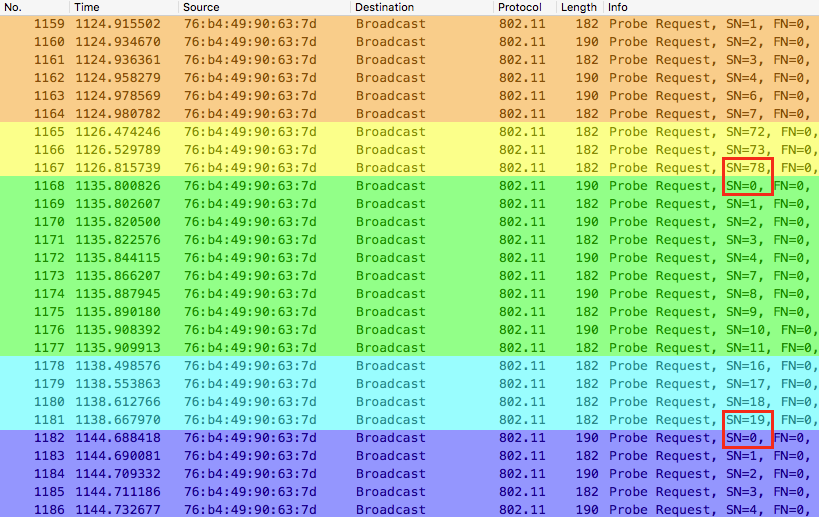
\includegraphics[width=\textwidth]{./img/result/randomization/ipad-mini}
	\end{table}

	% the SN
	\autoref{fig:ipad-random} depicts several examples of captured probe request packets from iPad mini, which were captured by Wireshark. The column represents, from left to right, the number of captured packet, the time of capture since beginning of capture (in second), the source address (\ac{MAC} address), the destination address, the communication protocol, packet length, and packet information.
	
	As we can see in~\autoref{fig:ipad-random}, the iPad mini reset the Sequence Number (\ac{SN}) after broadcasting two bursts of probe request. We can see in~\autoref{fig:ipad-random} that each burst, with nearly identical timestamp, is grouped in color. The red boxes mark the \ac{SN} reset, which mark a transition of \ac{SN} from 78 to 0, and 19 to 0.


	\subsection{Nexus 5X} % (fold)
	\label{sub:lg_nexus_5x}
	% when does the random mac appear?
	As opposed to iPad mini, Nexus 5X only sent out randomized \ac{MAC} address when the screen was off. When Nexus 5X woke up from sleep, it would immediately send out 4 or 10 probe request packets with real \ac{MAC} address. When Nexus 5X screen went off, Nexus 5X firstly sent out random \ac{MAC} address in every 2 to 10 seconds. Normally, Nexus 5X broadcast a burst of probe request packets roughly in each 60 seconds.

	Unlike iPad mini, Nexus 5X changed the \ac{MAC} address in each burst of probe request packets, as depicted in~\autoref{fig:nexus-random}. However, the first three octets were always the same and only the last three octets were changed. We can see that \verb|da:a1:19| appears in multiple bursts in~\autoref{fig:nexus-random} with different last three octets, \verb|ce:47:5f|, \verb|00:3f:25|, and \verb|b5:51:2c|, respectively.
	
	\begin{table}[h]
		\centering
		\caption[An example of captured probe requests from Nexus 5X.]{An example of captured probe requests from Nexus 5X in Wireshark. The colors mark out different bursts of probe request packets. The original \ac{MAC} address is indicated by cyan color in the last burst.}
		\label{fig:nexus-random}
		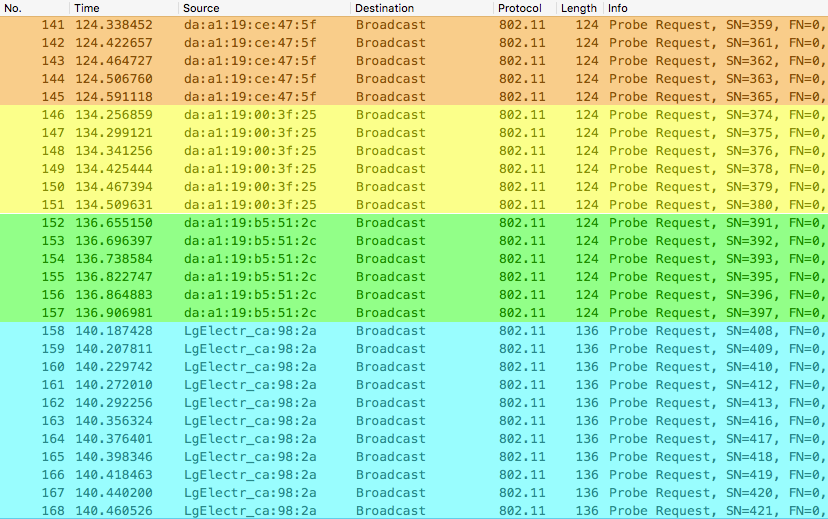
\includegraphics[width=\textwidth]{./img/result/randomization/nexus-5x}
	\end{table}	

	% the SN
	\autoref{fig:nexus-random}~depicts an example of captured probe request packets from Nexus 5X in the same format as~\autoref{fig:ipad-random}. There are four bursts of probe request packets marked in different colors. Three of the bursts are random \ac{MAC} address, while the last burst, marked in blue color, is the Nexus 5X original \ac{MAC} address.

	As we can see from~\autoref{fig:nexus-random}, the last probe request packet of a burst has a close \ac{SN} to the first packet of the next burst, although it is not sequential. We observed no obvious pattern in \ac{SN} change during the experiment.

	\subsection{Review} % (fold)
	\label{sub:review}
	% \added{
		Based on our findings in \ac{MAC} address randomization investigation, we can minimize the side-effect of \ac{MAC} address randomization by using one minute cycle length in data collection.
	% }
	This means we record the ambient noise and capture time-lapse images within 1 minute time interval, while we capture probe request packets in 52 seconds followed by two times of \ac{AP} scanning (see~\autoref{sub:scanning}).


% maybe use this
% Use table of simulation about randomized mac address using different time window.

\section{Correlation between Crowd Count and Sensor Readings} % (fold)
\label{sec:crowd_count_correlation-result}
In this section, we present the result of data collection using 1 minute cycle length, which consist of probe request packet capture, \ac{AP} scan, ambient noise recording, and time-lapse images capture (see~\autoref{fig:sensor-measurement}). As for the ground truth estimation, we used head count of time-lapse images and device count in unique \ac{MAC} address in probe request. The results indicate whether smartphone sensor readings can be an approach to estimate the level of social density or crowd count.

% when
We collected the data from Wednesday, October 26\textsuperscript{th} 2016, to Saturday, October 29\textsuperscript{th} 2016. The timing of data collection is shown in~\autoref{tab:location-summary}. During the data collection, we observed no special events in which the social density level are much higher than the normal condition, especially in public places, such as Grote Markt and Paddepoel shopping center.

% assumption
In manual head counting, a person might appear more than once, i.e., the person was captured in multiple GoPro cameras, because we took time-lapse images and some people were actively moving. We make sure that the people who appear several times in different images are counted exactly once. Furthermore, sometimes we captured vehicles with very limited visual appearance of the people inside. We assume that there are a person in a car and five people in a bus. We present some examples of time-lapse images in~\autoref{ch:appendix-time-lapse-images}.

\begin{figure}[h]
	\begin{adjustwidth}{-2cm}{}
	\centering
	\subfloat[head count]{
		\label{fig:population-head-count}{
			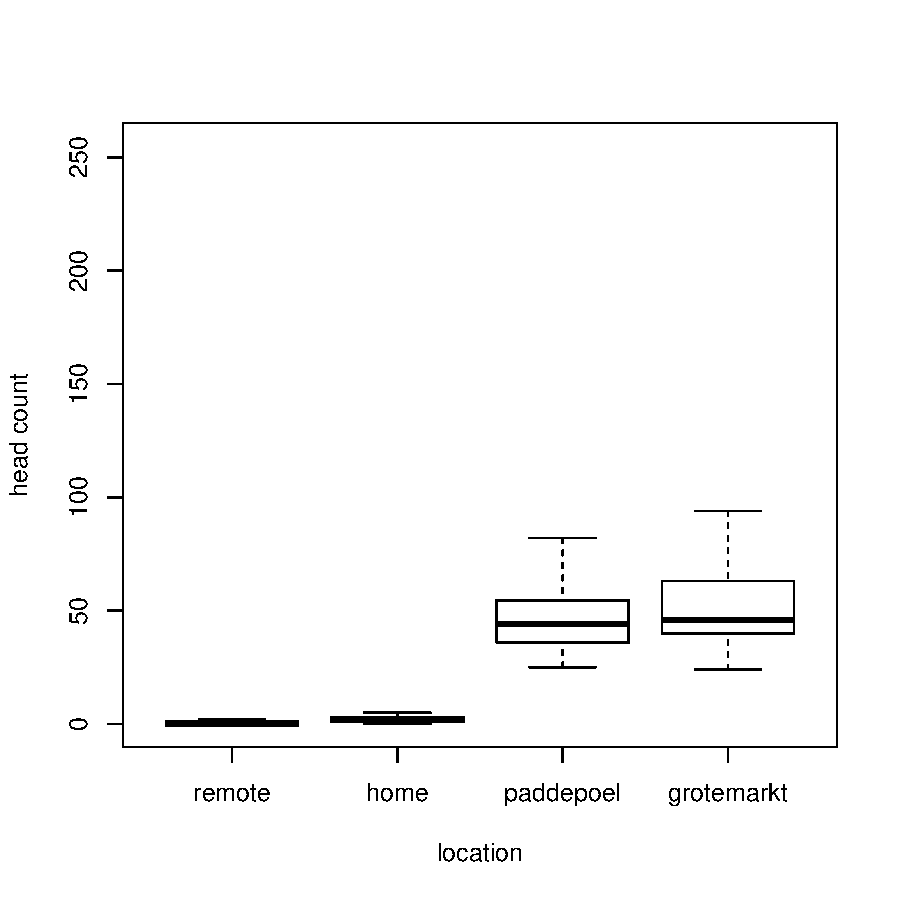
\includegraphics[width=0.65\textwidth]{./img/result/boxplot-hc-small}
		}
	}
	\subfloat[device count]{
		\label{fig:population-device-count}{
			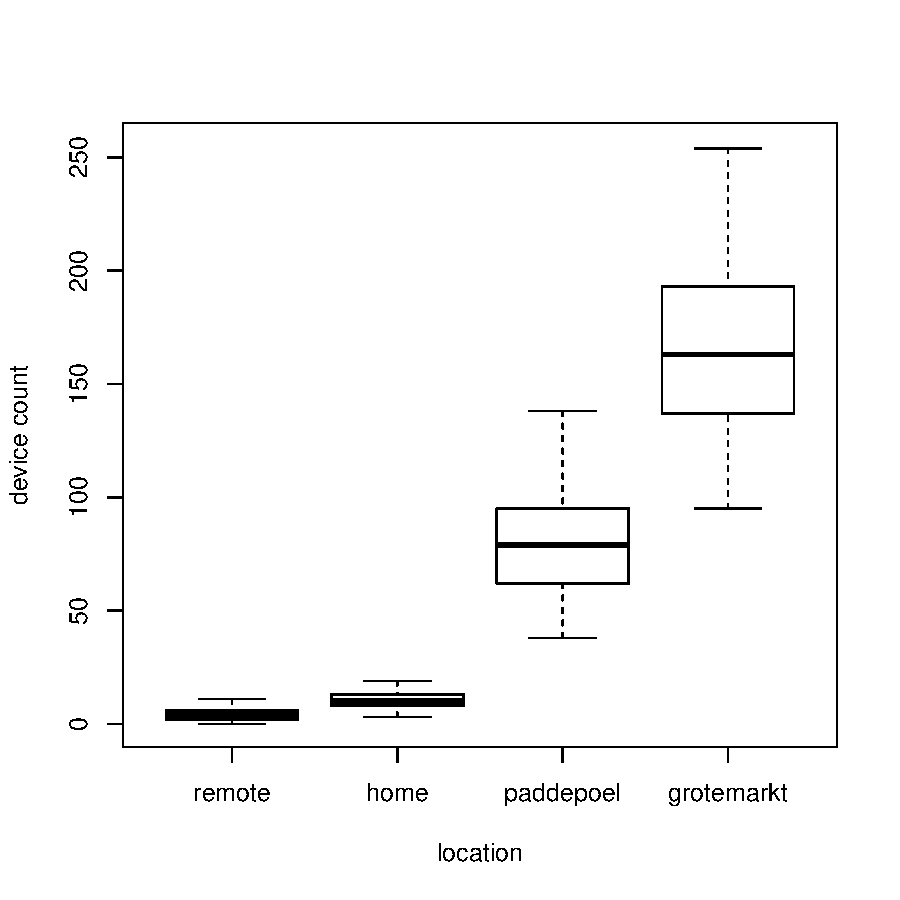
\includegraphics[width=0.65\textwidth]{./img/result/boxplot-dc-small}
		}
	}
	\end{adjustwidth}
	\caption[A box plot of the population]{A box plot showing the population of estimated social density in each location by head count (\ref{fig:population-head-count}) and device count (\ref{fig:population-device-count}).}
	\label{fig:total-population}
\end{figure}

We present the important results of the experiment, such as the variation of the social density level, example of ambient noise recording, correlation of \ac{AP} count and sensor readings, the effect of scanning time, and all parameters used for analysis. The appendices present the detailed results, such as the sensor readings both in scatter plot and line chart (\autoref{ch:appendix-sensor-readings}), example of time-lapse images for each location (\autoref{ch:appendix-time-lapse-images}), and ambient noise recording (\autoref{ch:appendix-ambient-noise}).

\autoref{fig:total-population}~depicts the variation of the estimated social density level in each location, e.g., the lowest value, the first quartile, the median, the upper quartile, and the maximum value. The value are estimated by two approximation, namely head count (\ref{fig:population-head-count}) and device count (\ref{fig:population-device-count}).

As we can see in~\autoref{fig:total-population}, the maximum value of the device count based estimation is higher than the head count based estimation. For instance, in Grote Markt, the maximum value of device count is 288, while the maximum value of head count is 115. However, both estimations are showing the same trend, which says that Grote Markt has the highest social density level and remote area has the lowest social density level.

% device count
%    LOC Min  Q1 Med  Q3 Max
% 1:   r   0   2   4   6  11
% 2:   h   3   8  10  13  46
% 3:   p  38  62  79  95 150
% 4:   g  95 137 163 193 288

% head count
%    LOC Min Q1 Med   Q3 Max
% 1:   r   0  0   0  1.0   4
% 2:   h   0  1   2  3.0   5
% 3:   p  25 36  44 54.5  95
% 4:   g  24 40  46 63.0 115











	\subsection{Ambient Noise Recordings} % (fold)
	\label{sub:ambient_noise_recordings}
	As an example of ambient noise recording, \autoref{tab:ambient-noise-average-day4} and \autoref{fig:audio-result-day4} show the result of ambient noise recording in day 4, when more crowds were present than any other days. We measure the ambient noise in decibels (dB). In this unit, the closer the value to zero, the louder the sound (noise). We take two measures of ambient noise to characterize the surrounding, namely Peak Level (\ac{PKLV}), which is the highest value of a total waveform, and Root Mean Square (\ac{RMS}), which is the effective value or the mean of an audio recording. \ac{PKLV} and \ac{RMS} are positively correlated but \ac{RMS} is more stable than \ac{PKLV}.

	\begin{table}[H]
	\centering
	\caption[]
	{The average of RMS and PKLV of ambient noise recording in day 4.}
	\label{tab:ambient-noise-average-day4}
	\begin{tabular}{lll}
	\toprule
	            & \ac{RMS} (dB) & \ac{PKLV} (dB) \\ \midrule
	Remote area &  -47.74           &  -26.90    \\
	Home        &  -39.39         & -12.84       \\
	Paddepoel   & -26.54          &  -3.39       \\
	Grote markt & -36.29             & -5.87     \\ \bottomrule
	\end{tabular}
	\end{table}

	\begin{figure}[H]
		% \centering
		\subfloat[peak level]{
			\label{fig:peak-level-day4}{
				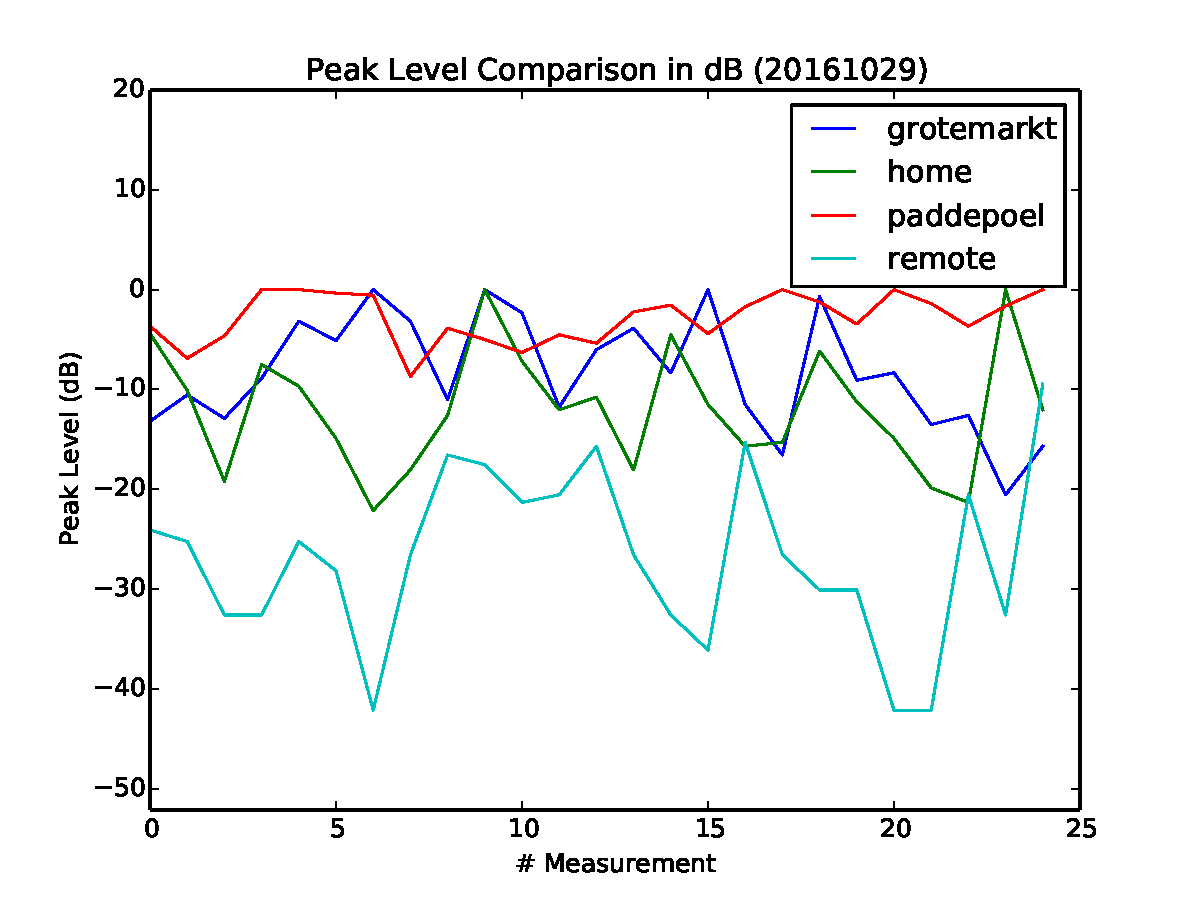
\includegraphics[width=0.8\textwidth]{./img/result/sound/peak-level-comparison-20161029}
			}
		}\\
		\subfloat[root mean square]{
			\label{fig:rms-day4}{
				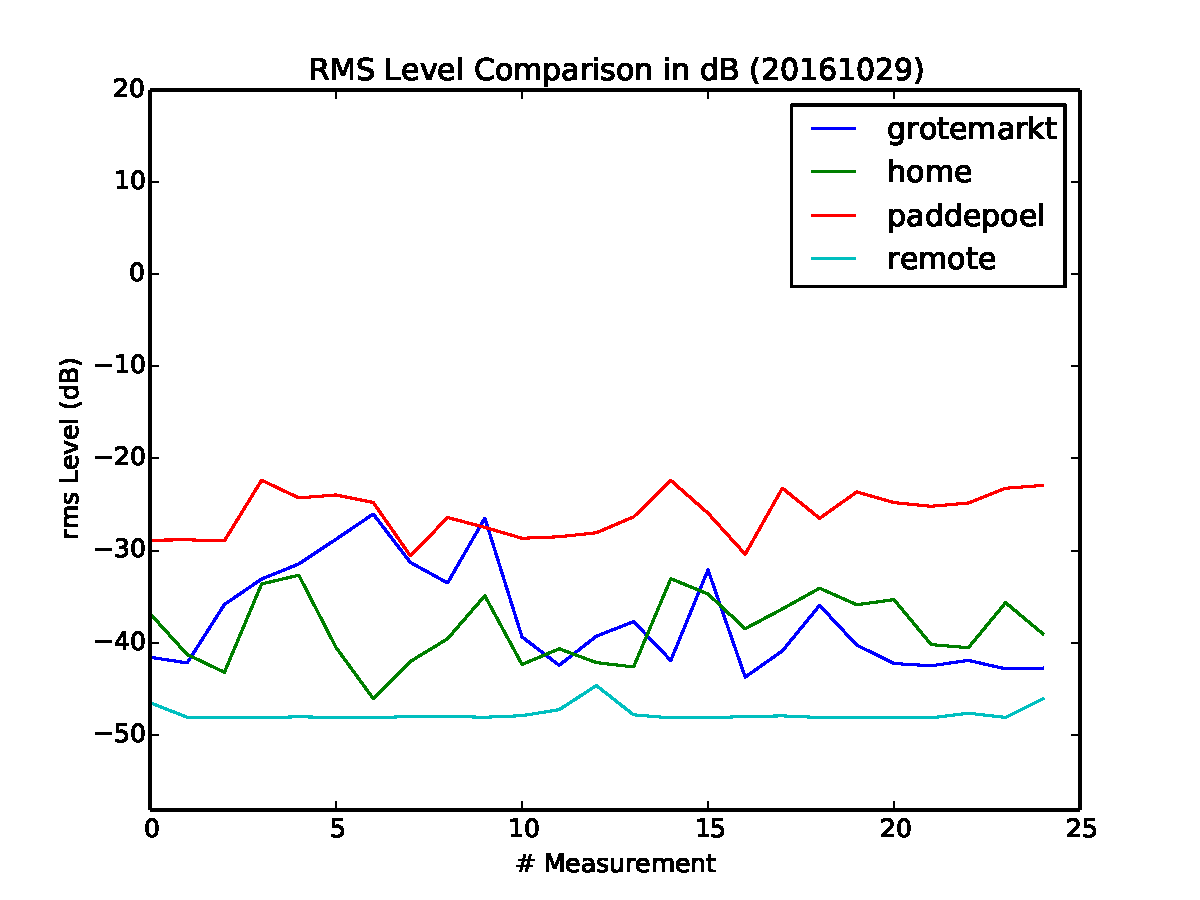
\includegraphics[width=0.8\textwidth]{./img/result/sound/rms-level-comparison20161029}
			}
		}
		\caption[Line chart of ambient noise at day 4]{Line chart showing the peak level (\ref{fig:peak-level-day4}) and root-mean-square (\ref{fig:rms-day4}) of the ambient noise recording in each cycle at day 4.}
	\label{fig:audio-result-day4}
	\end{figure}

	As we can see in the average value (\autoref{tab:ambient-noise-average-day4}) or line chart (\autoref{fig:audio-result-day4}), more crowded place has higher ambient noise value. We see that remote area is the quietest location, with -47.74 dB of average \ac{RMS}, while Paddepoel is the noisiest location, with -26.54 dB of average \ac{RMS}. As for the line chart, we can see more overlaps in \ac{PKLV} (\autoref{fig:peak-level-day4}) than in \ac{RMS} (\autoref{fig:rms-day4}). The \ac{RMS} of remote area is stable near -50.00 dB. We can also see the same trends for the rest of the ambient noise recordings, although some overlaps are present, as shown in~\autoref{ch:appendix-ambient-noise}.


	% \subsubsection{Speaker Count Extraction} % (fold)
	% \label{ssub:probe_request_based_estimation}
	% In~\autoref{sec:line_charts}, we present the result of smartphone sensor readings that displays the estimated speaker count from ambient noise recording, extracted using unsupervised machine learning method by Xu, et al,~\cite{thesis067}. However, the result is not satisfying as the speaker count estimation is mostly yielding zero speaker count, even in the most crowded location. When we listened to the audio recording, sometimes human voice is present but not apparent and clear.

	% To test the accuracy of unsupervised speaker count estimation from Xu, et al,~\cite{thesis067}, we apply the algorithm to audio recordings in which the speaker voice is apparent and clear. We select different audio recordings that have diverse speaker count, ranging from single speaker, as in a speech or monologue, two speakers, as in duets or interview, and five speakers, as in a cappella.

	% We tune two parameters in the speaker count algorithm, namely ${\theta}_{s}$ and ${\theta}_{d}$, using recommended configuration in their implementation of the algorithm\footnote{\url{https://github.com/lendlice/crowdpp}}. The ${\theta}_{s}$ parameter refers to the confidence level that we can identify the same speaker, while ${\theta}_{d}$ is about new speaker. \autoref{tab:speaker-count-result} summarizes the result.

	% \begin{table}[h]
	% \begin{adjustwidth}{-2cm}{}
	% \centering
	% \caption{Speaker count result}
	% \label{tab:speaker-count-result}
	% \begin{tabular}{l|l|llllll}
	% \toprule
	% \multirow{2}{*}{Description} & \multirow{2}{*}{\specialcell{Total\\Speaker(s)}} & \multicolumn{6}{c}{Detected Speaker(s) (${\theta}_{s},{\theta}_{d}$)} \\
	%                              &                                & (13, 18) & (14, 24) & (15.6, 21.6) & (16, 21) & (17, 22) & (18, 25) \\ \midrule
	% speech                     & 1 & 11 & 5 & 6 & 7 & 6 & 5 \\
	% monologue                    & 1 & 5 & 4 & 5 & 5 & 5 & 3 \\
	% duets                        & 2 & 1 & 1 & 1 & 1 & 1 & 1 \\
	% interview     			 & 2 & 5 & 5 & 5 & 5 & 5 & 5 \\
	% a cappella                   & 5 & 5 & 4 & 4 & 4 & 4 & 4 \\
	% \bottomrule 
	% \end{tabular}
	% \end{adjustwidth}
	% \end{table}

	% We can see from~\autoref{tab:speaker-count-result} that the speaker estimation is not accurate. The only accurate estimation is done using 13 and 18 as the ${\theta}_{s}$ and ${\theta}_{d}$, respectively, but it only applies to a cappella recording with five speakers. The estimation gives stable result for duets and interview recording along different combination of ${\theta}_{s}$ and ${\theta}_{d}$, although it is not correct. 







	\subsection{AP and Social Density Correlation} % (fold)
	\label{sub:ap_and_social_density_correlation}
	We are particularly interested in seeing the trend and correlation of WiFi \ac{AP} count and social density level, estimated by head count and device count. We draw a scatter plot of \ac{AP} count vs device count and \ac{AP} count vs head count separately, as well as device count vs head count to see the correlation of the two social density estimation. The plots are shown in~\autoref{fig:scatter-dc-ap}, \autoref{fig:scatter-hc-ap}, and \autoref{fig:scatter-hc-dc}. We also present the line chart of the readings in~\autoref{ch:appendix-sensor-readings}.

	\autoref{fig:scatter-dc-ap} depicts the correlation of device count and \ac{AP} count. The data plotted in~\autoref{fig:scatter-dc-ap} come from all data from four days of experiments. The location is coded in color so that we can distinguish which data come from which location. The plots of the correlation separately in each day are also available in~\autoref{ch:appendix-sensor-readings}, shown in~\autoref{fig:ap-dc-scatterplot}.
	
	As we can see in~\autoref{fig:scatter-dc-ap} there is a positive trend that indicates both variables have a positive correlation. This means when the \ac{AP} count increases, the device count, which points to social density level, increases as well. The correlation coefficient $\rho$ is 0.877, indicating a strong correlation, and the $p$-value is below 0.05, indicating that the result is significant.
	% \added{
		Each location forms a distinguishable cluster, although some overlaps are present.
	% }
	The cluster of home and remote are close and the cluster of Paddepoel and Grote Markt are adjacent. However, there is a gap that separates home-remote cluster and Paddepoel-Grote markt cluster.

	% all result - device count
	\begin{figure}[h]
		\centering
		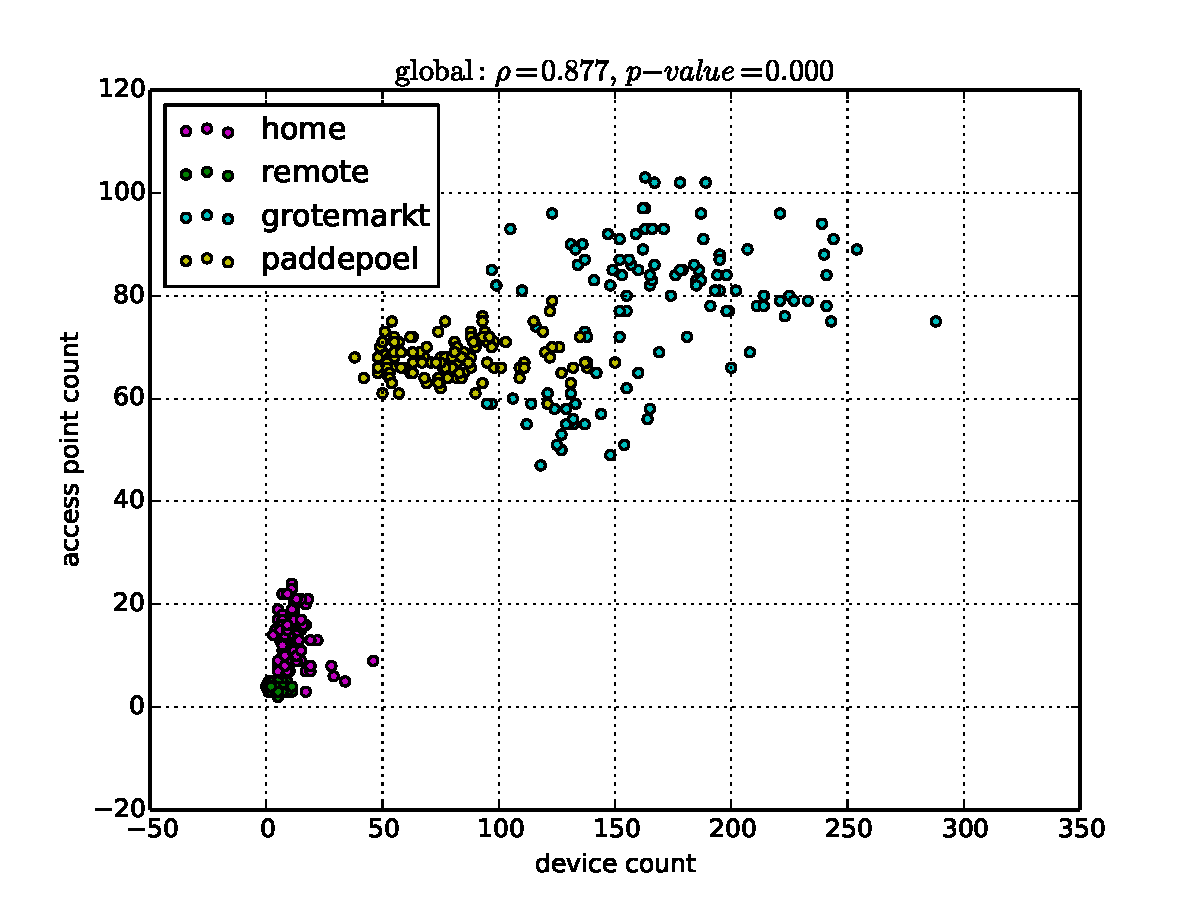
\includegraphics[width=0.8\textwidth]{./img/result/global-pr-vs-ap}
		\caption[Scatter plot of device and \ac{AP} count.]
		{Scatter plot showing the correlation between \textit{device count} and \textit{\ac{AP} count} of all collected data. The locations are marked in different color. The correlation coefficient is $\rho=0.877$.}
		\label{fig:scatter-dc-ap}
	\end{figure}

	\autoref{fig:scatter-hc-ap} portrays the correlation between head count and \ac{AP} count of data collected in four days of all location. \autoref{fig:scatter-hc-ap} uses the same color coding as~\autoref{fig:scatter-dc-ap} to distinguish the location. The plots showing the correlation in separate days are available in~\autoref{ch:appendix-sensor-readings}, shown in~\autoref{fig:ap-hc-scatterplot}.
	
	We can see similar trend in~\autoref{fig:scatter-hc-ap}. The correlation is strong, indicated by correlation coefficient $\rho = 0.877$, and significant, indicated by p-value which is below 0.05. However, the Grote Markt and Paddepoel clusters are overlapping each other. A gap between remote-home cluster and Grote Markt-Paddepoel cluster is also present.

	% all result - head count
	\begin{figure}[H]
		\centering
		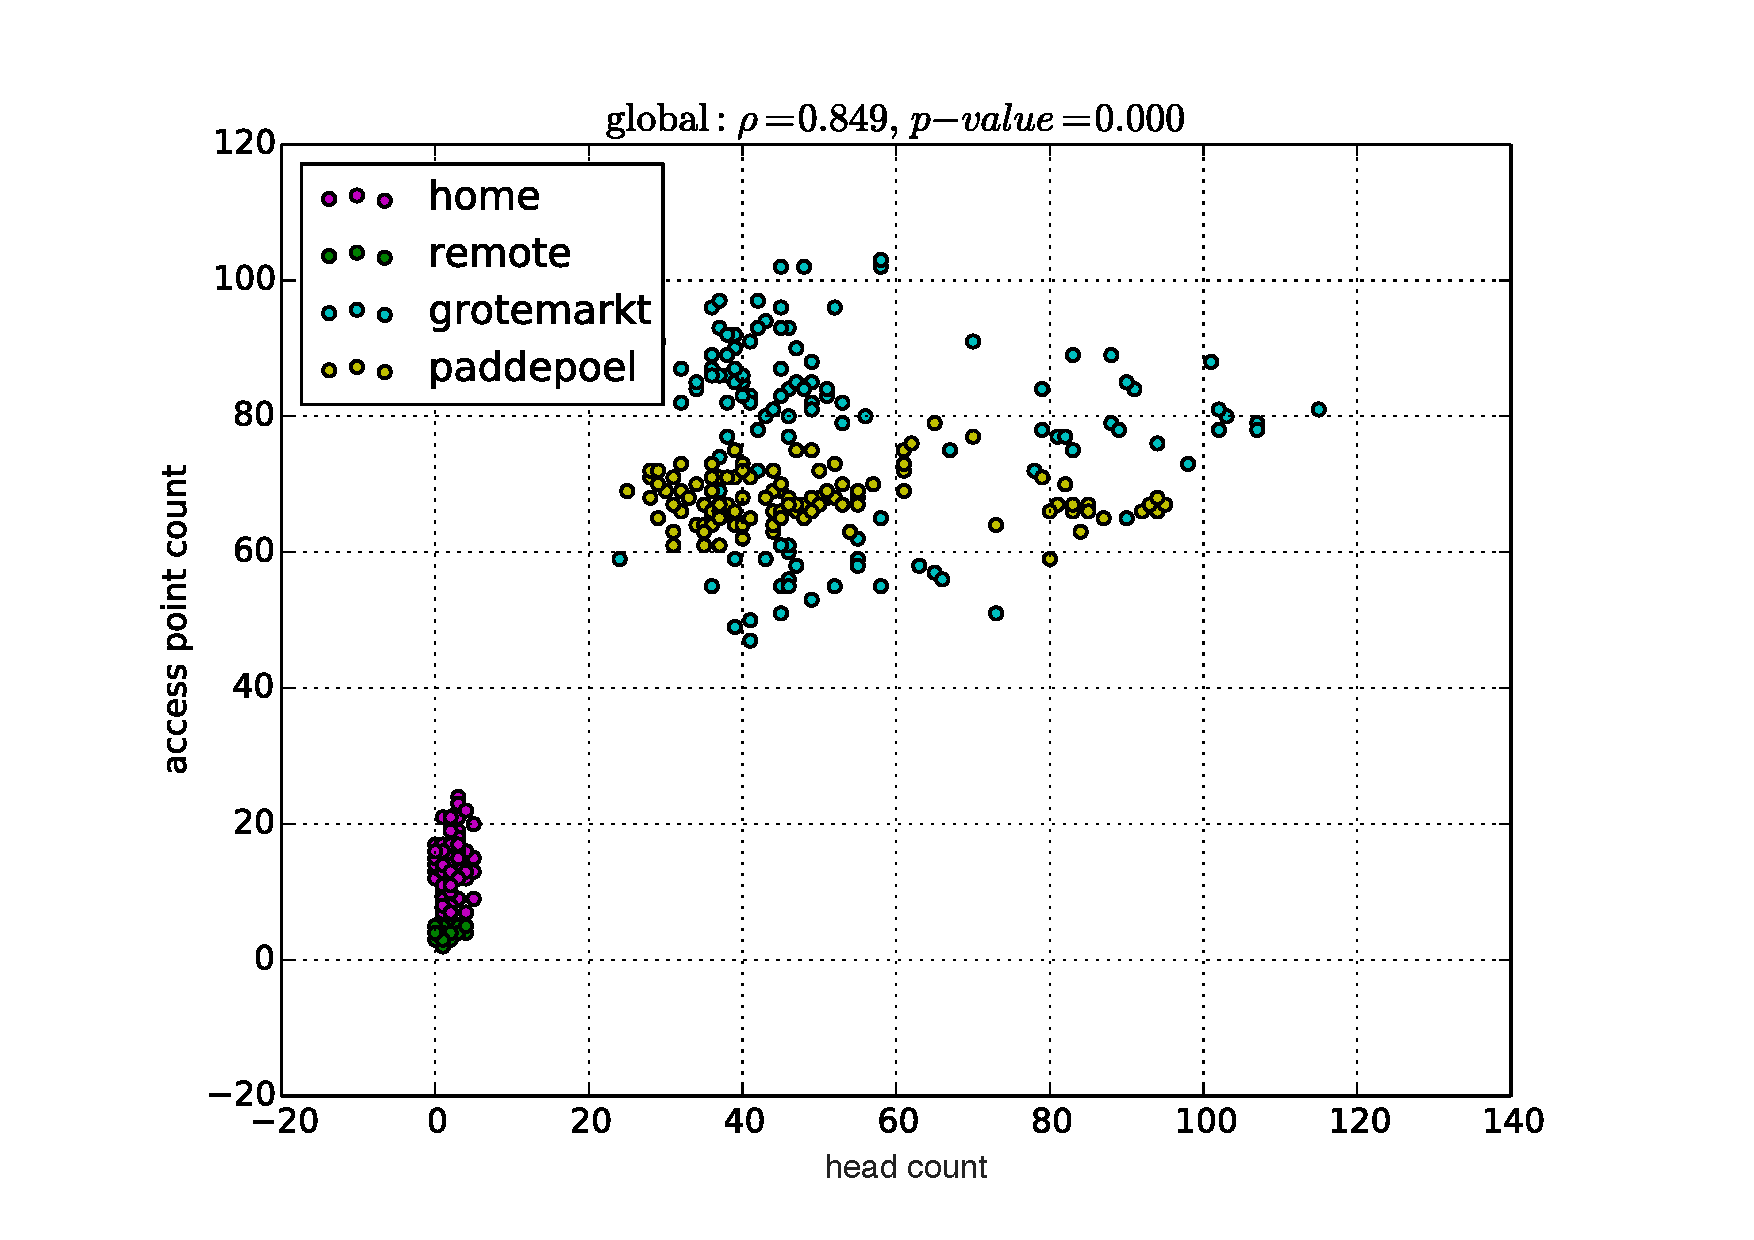
\includegraphics[width=0.8\textwidth]{./img/result/global-gt-vs-ap}
		\caption[Scatter plot of head and \ac{AP} count.]
		{Scatter plot showing the correlation between \textit{head count} and \textit{\ac{AP} count} of all collected data. The locations are marked in different color. The correlation coefficient is $\rho=0.849$.}
		\label{fig:scatter-hc-ap}
	\end{figure}

	\autoref{fig:scatter-hc-dc} shows the correlation of head count and device count of all collected data. The locations are coded in color as well. Head count and device count have a strong correlation, marked by the correlation coefficient $\rho$, which is 0.857. A gap between remote-home cluster and Grote Markt-Paddepoel cluster is also present, although it is narrower than the gap in \autoref{fig:scatter-dc-ap} and \autoref{fig:scatter-hc-ap}. \autoref{fig:hc-dc-scatterplot} in \autoref{ch:appendix-sensor-readings} presents the scatter plots showing the correlation of head count and device count in each day of the experiment.

	% all result - device count vs head count
	\begin{figure}[H]
		\centering
		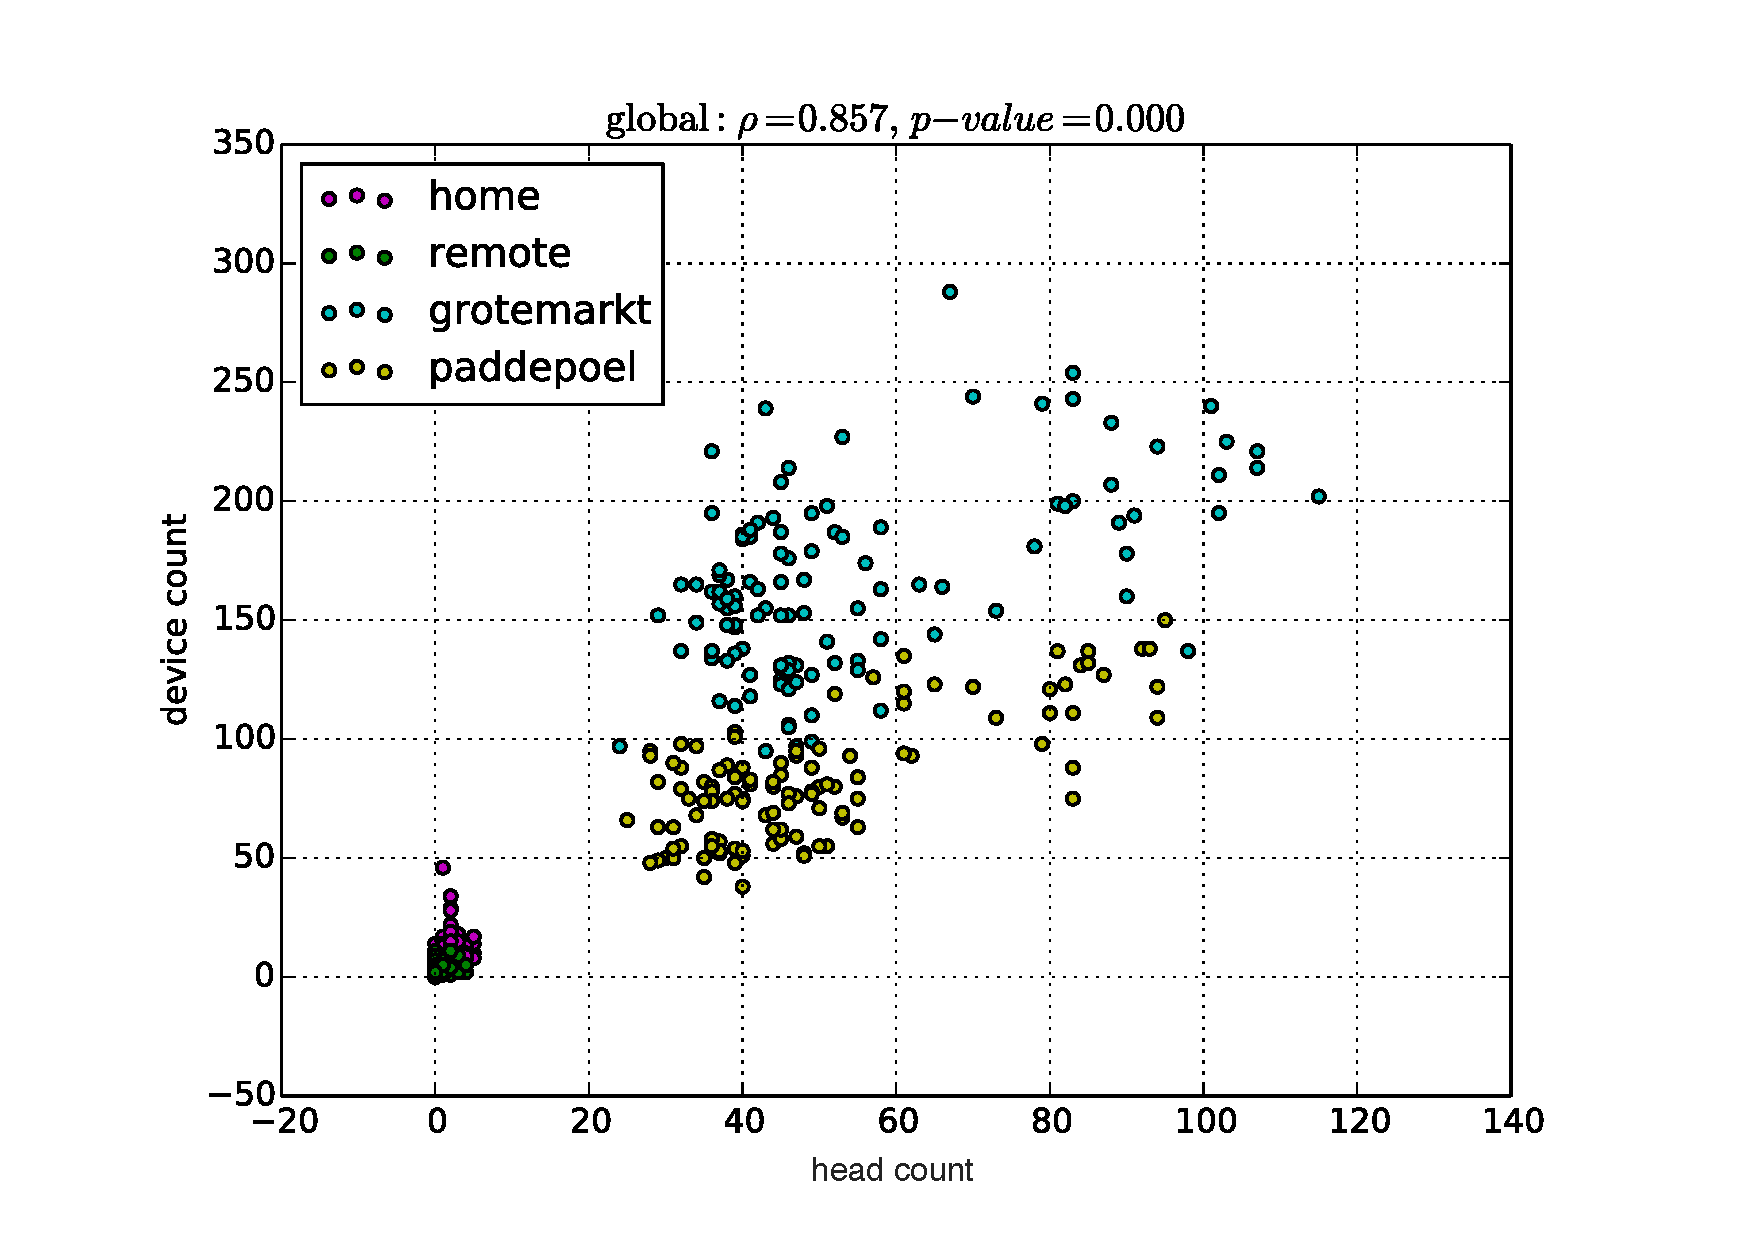
\includegraphics[width=0.8\textwidth]{./img/result/global-gt-vs-pr}
		\caption[Scatter plot of head and device count.]
		{Scatter plot showing the correlation between \textit{head count} and \textit{device count} of all collected data. The locations are marked in different color. The correlation coefficient is $\rho=0.857$.}
		\label{fig:scatter-hc-dc}
	\end{figure}

	As we can see in three scatter plots (\autoref{fig:scatter-dc-ap}, \autoref{fig:scatter-hc-ap}, and \autoref{fig:scatter-hc-dc}), \ac{AP} and social density level from both head count and device count have a positive correlation. The correlation is strong, which is roughly 0.8 with p-value less than 0.05. 






	\subsection{Effect of Scanning Time} % (fold)
	\label{sub:effect_of_scanning_time}
	We performed four experiments on Sunday, October 30\textsuperscript{th} 2016, to investigate the effect of scanning time to the \ac{AP} count and social density correlation. We collected the data for 45 minutes, consisting WiFi and audio data, in four different scanning time, namely
	\begin{enumerate*}[label={\alph*)},font={\color{red!50!black}\bfseries}]
	  \item 09:00,
	  \item 12:00,
	  \item 15:00,
	  \item and 18:00
	\end{enumerate*}.
	
	\autoref{fig:time-effect} shows the WiFi scanning result in four separate line charts. Each chart depicts the result of a certain scanning time. The blue lines, which depict the \ac{AP} count, fluctuate stably around 100, while the green lines, which represent the device count, have a big variance. As we can see in~\autoref{fig:grotemarkt-0900}, the green line is fluctuating below the blue line, indicating there were less device than available \ac{AP} count. However, in~\autoref{fig:grotemarkt-1200}, \autoref{fig:grotemarkt-1500}, and \autoref{fig:grotemarkt-1800}, the condition changes. The green lines surpass the blue lines, which indicates that the number of device was increased. \autoref{fig:grotemarkt-1500} shows an increasing trend of device count, while \autoref{fig:grotemarkt-1800} shows a decreasing trend.

	\begin{figure}[H]
		\centering
		\begin{adjustwidth}{-3cm}{}
		\subfloat[09:00h]{
		  \label{fig:grotemarkt-0900}{
		    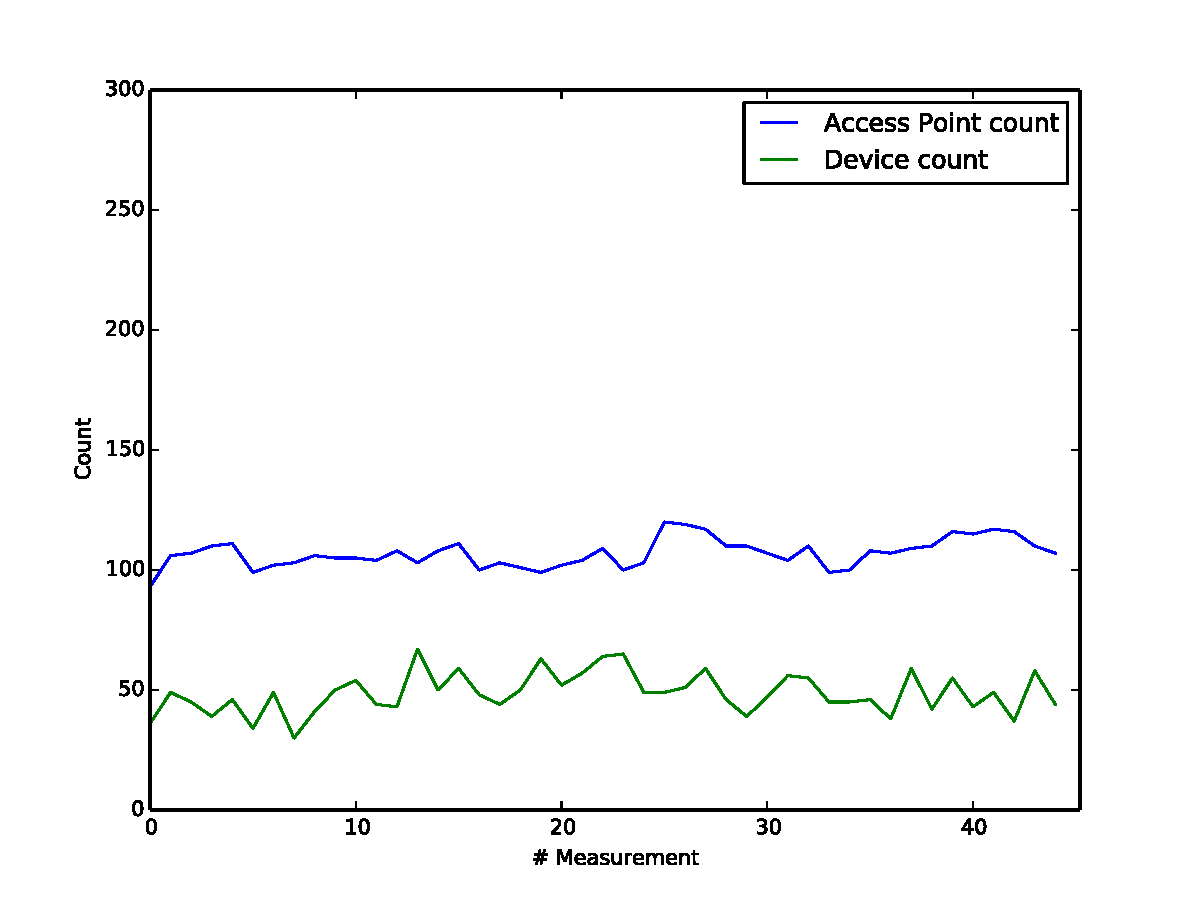
\includegraphics[width=0.7\textwidth]{./img/result/time/grotemarkt-0900}
		  }
		}
		\subfloat[12:00h]{
		  \label{fig:grotemarkt-1200}{
		    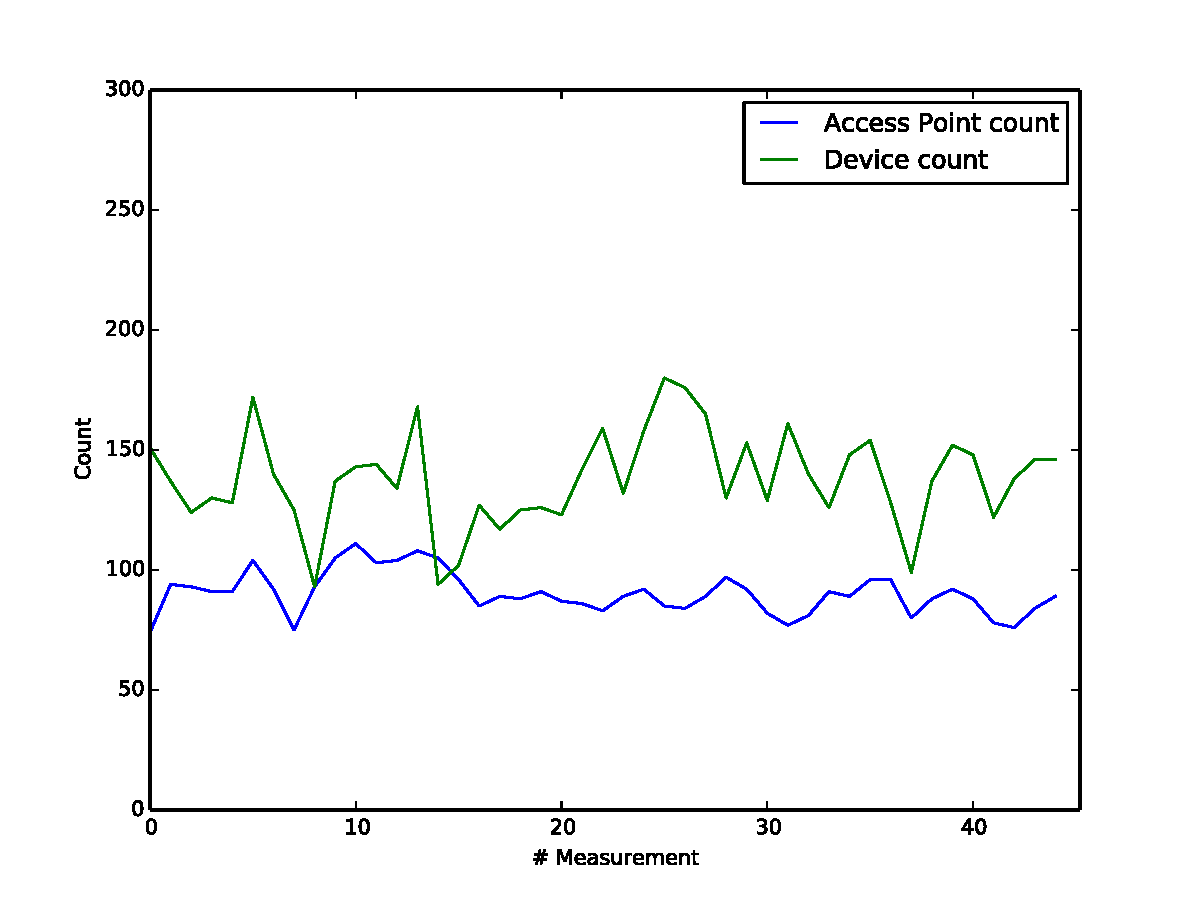
\includegraphics[width=0.7\textwidth]{./img/result/time/grotemarkt-1200}
		  }
		}\\
		\subfloat[15:00h]{
		  \label{fig:grotemarkt-1500}{
		    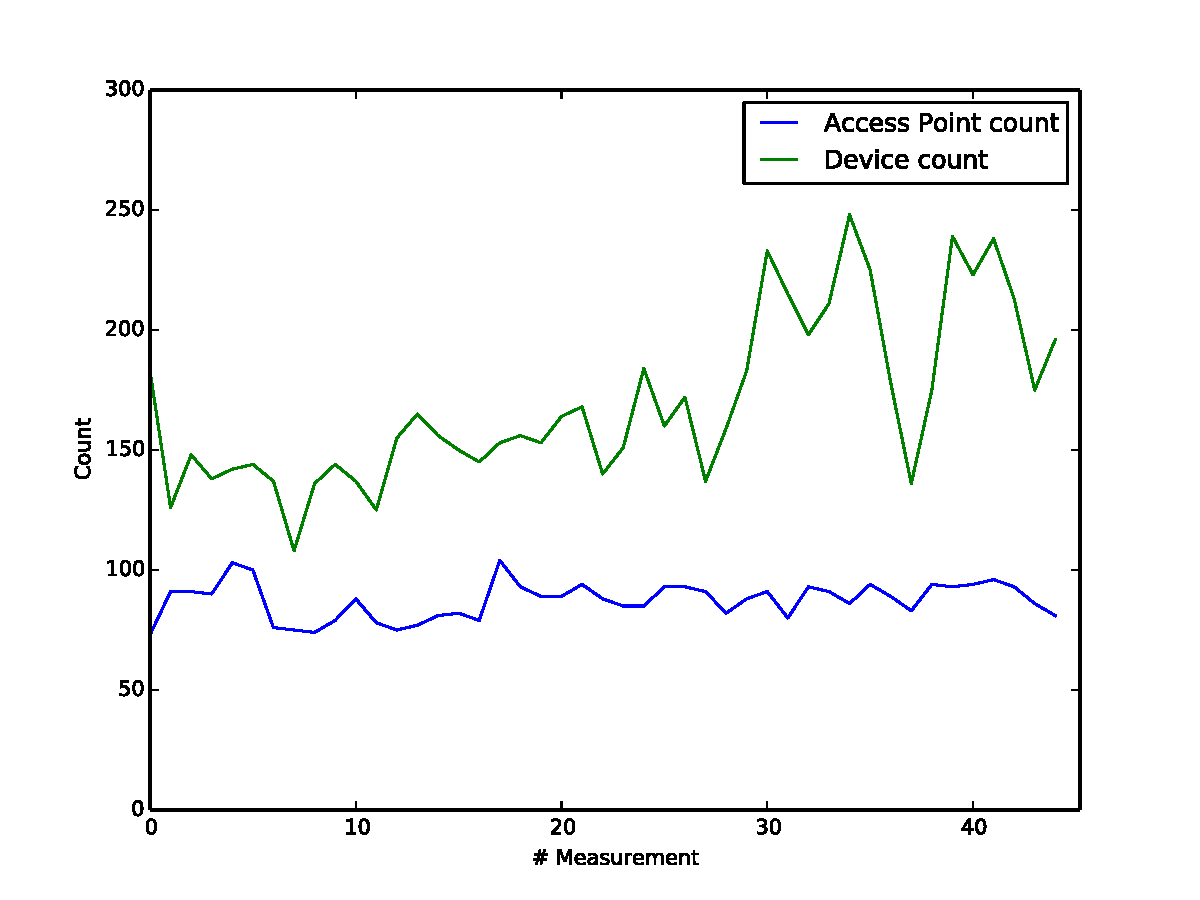
\includegraphics[width=0.7\textwidth]{./img/result/time/grotemarkt-1500}
		  }
		}
		\subfloat[18:00h]{
		  \label{fig:grotemarkt-1800}{
		    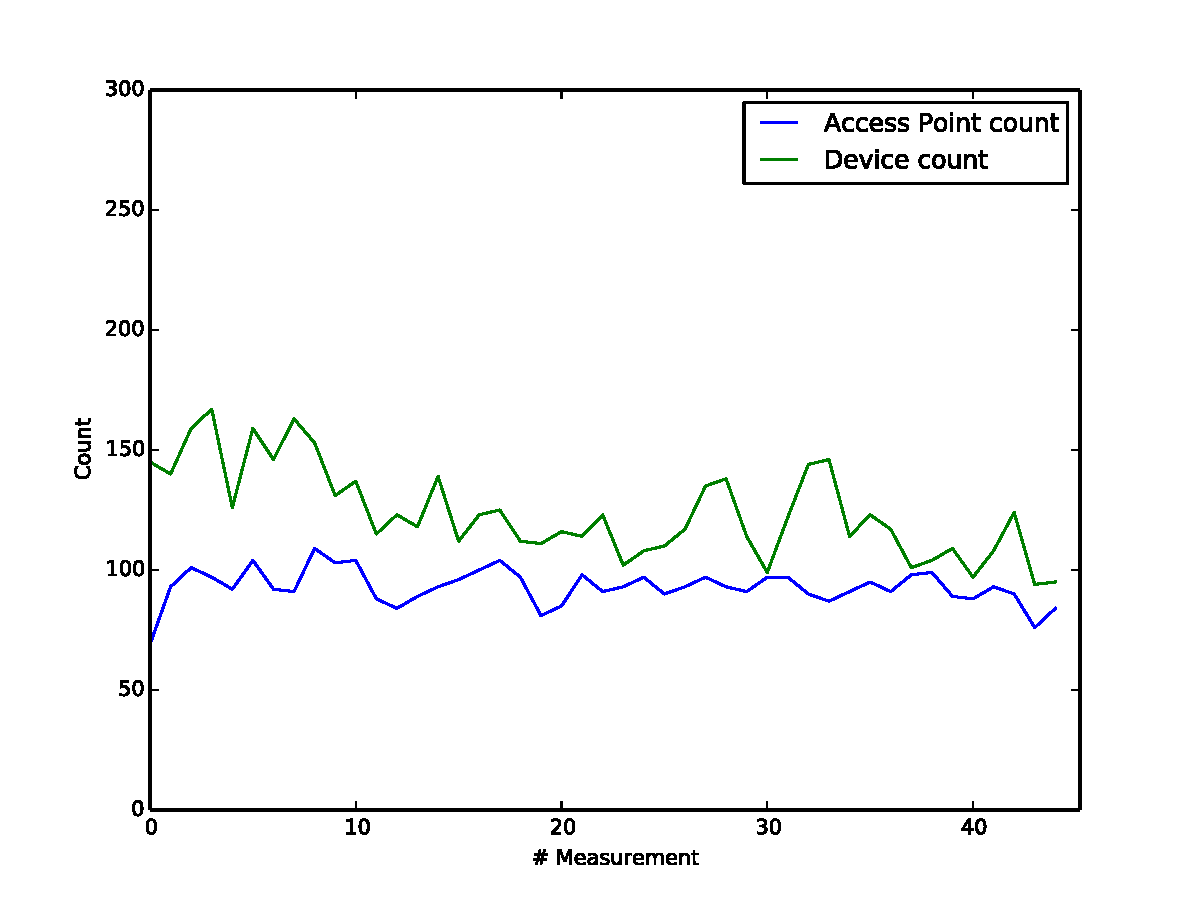
\includegraphics[width=0.7\textwidth]{./img/result/time/grotemarkt-1800}
		  }
		}
		\caption[Line charts of ambient noise on October 30, 2016.]
		{Line charts showing the \ac{AP} count (blue) and device count (green) in different data collection time at Grote Markt, Groningen, on October 30, 2016.}
		\label{fig:time-effect}
		\end{adjustwidth}
	\end{figure}

	% \added{
	Moreover, we present the ambient noise recording of the Sunday, October 30\textsuperscript{th} 2016 experiment in~\autoref{tab:ambient-noise-timely} and \autoref{fig:audio-result-timely}. If we look at the line charts (\autoref{fig:audio-result-timely}), the lines are mostly overlapping each other, making it difficult to distinguish the noise characteristics of each scanning time. However, the ambient noise summary in~\autoref{tab:ambient-noise-timely} presents more understandable characteristics. We see that, in \ac{PKLV}, the noise is increasing from 09:00h, peaking at 15:00h, and going back down at 18:00h. The ambient noise recordings are correlated with the WiFi scanning results presented in~\autoref{fig:time-effect}.

	\begin{table}[h]
	\centering
	\caption[The average of RMS and PKLV of ambient noise in four scanning time.]
	{The average of root-mean-square and peak level of ambient noise recording in four different scanning time.}
	\label{tab:ambient-noise-timely}
	\begin{tabular}{lll}
	\toprule
	       & \ac{RMS} (dB) & \ac{PKLV} (dB) \\ \midrule
	09:00h & -40.51        & -14.95          \\
	12:00h & -40.91        & -13.08          \\
	15:00h & -37.53        & -8.90           \\
	18:00h & -40.62        & -12.41          \\ \bottomrule
	\end{tabular}
	\end{table}

	\begin{figure}[h]
		% \centering
		\begin{adjustwidth}{-1cm}{}
		\subfloat[peak level]{
			\label{fig:peak-level-timely}{
				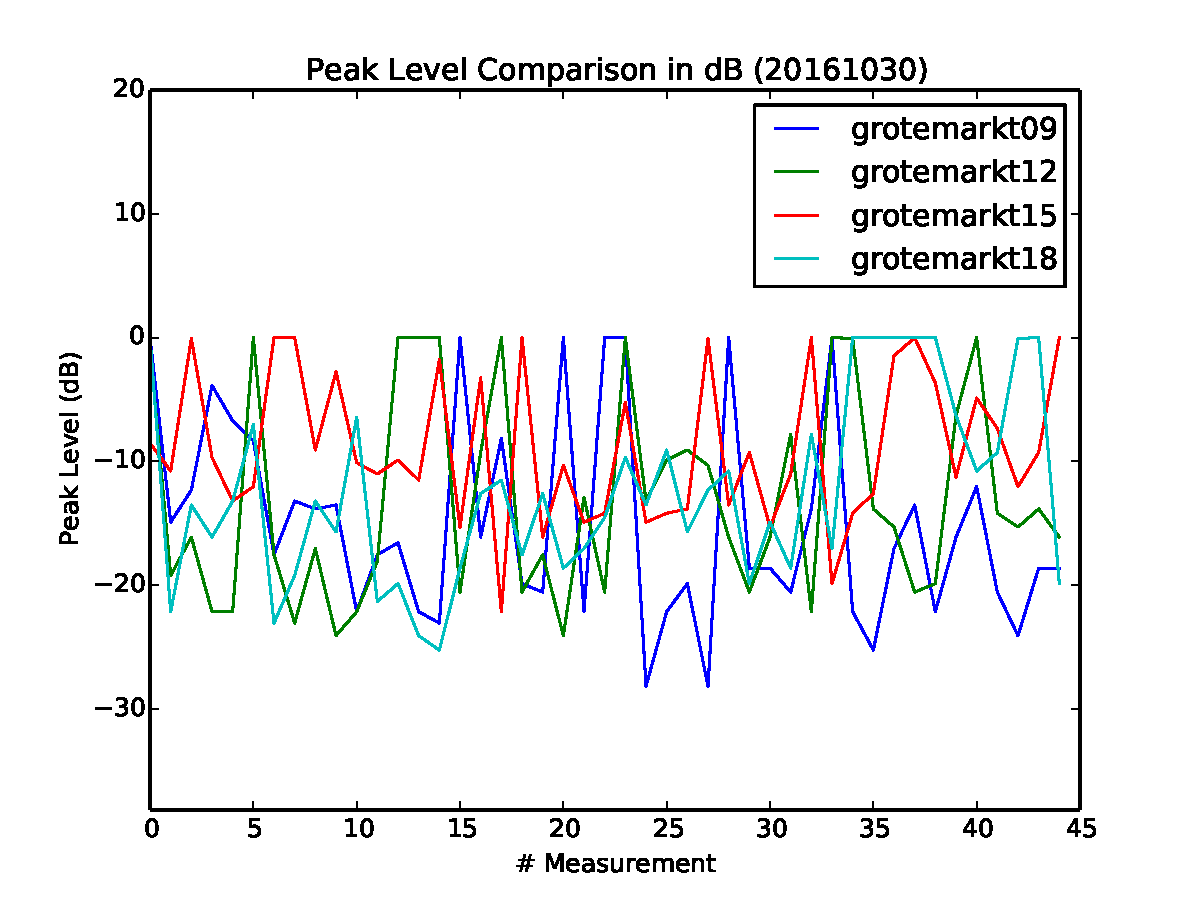
\includegraphics[width=0.6\textwidth]{./img/result/time/peak-level-comparison}
			}
		}
		\subfloat[root mean square]{
			\label{fig:rms-timely}{
				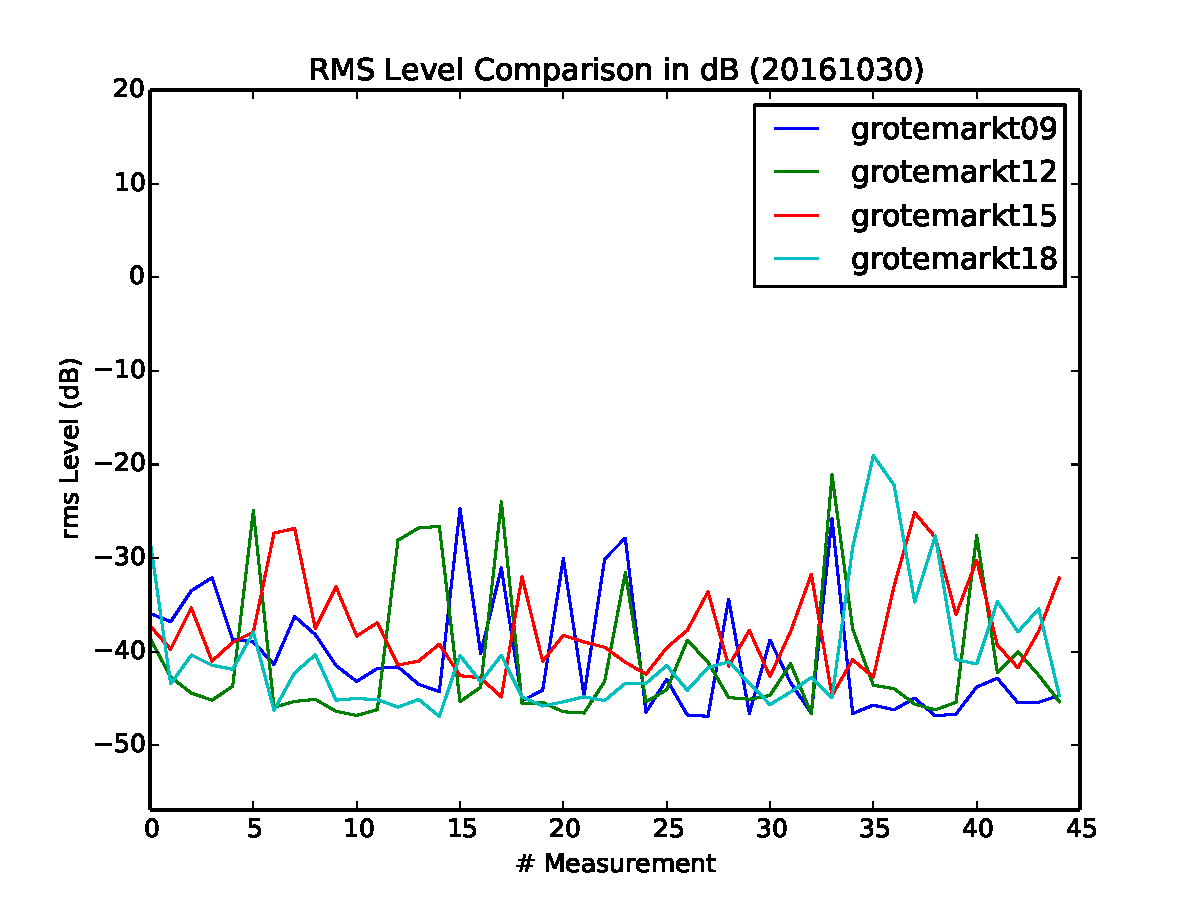
\includegraphics[width=0.6\textwidth]{./img/result/time/rms-level-comparison}
			}
		}
		\caption[Ambient noise in different scanning time.]
		{Line charts showing the peak level (\ref{fig:peak-level-timely}) and root-mean-square (\ref{fig:rms-timely}) of the ambient noise recording in four diffent scanning time.}
		\label{fig:audio-result-timely}
		\end{adjustwidth}
	\end{figure}
	% }



	\subsection{All Result} % (fold)
	\label{sub:all_result}
	\autoref{fig:scatterplot-matrix} shows all data collected in four days of experiments in a scatter plot matrix. In the lower left part are the scatter plots of each parameter correlation along with the Lowess curve fitted to the data. In the upper part are the correlation coefficient and the p-value. Along the diagonal are the histograms and the labels of each parameter.

	There are eight parameters extracted from all datasets of four days experiment. The \ac{AP}, \ac{RSSI}, \ac{DC}, and \ac{SNR} parameters are from WiFi based readings. \ac{AP} is the count of available \ac{AP} that a smartphone can get, while \ac{RSSI} is the average of the signal strength of the \ac{AP}. \ac{DC} is the device count, based on unique \ac{MAC} address, and \ac{SNR} is the average of signal-to-noise ratio of the captured probe request packets. \ac{SC}, \ac{RMS}, and \ac{PKLV} are from recorded ambient noise, while \ac{HC} is from manual head counting of time-lapse images.

	\begin{figure}[h]
		\begin{adjustwidth}{-3cm}{}
		\centering
		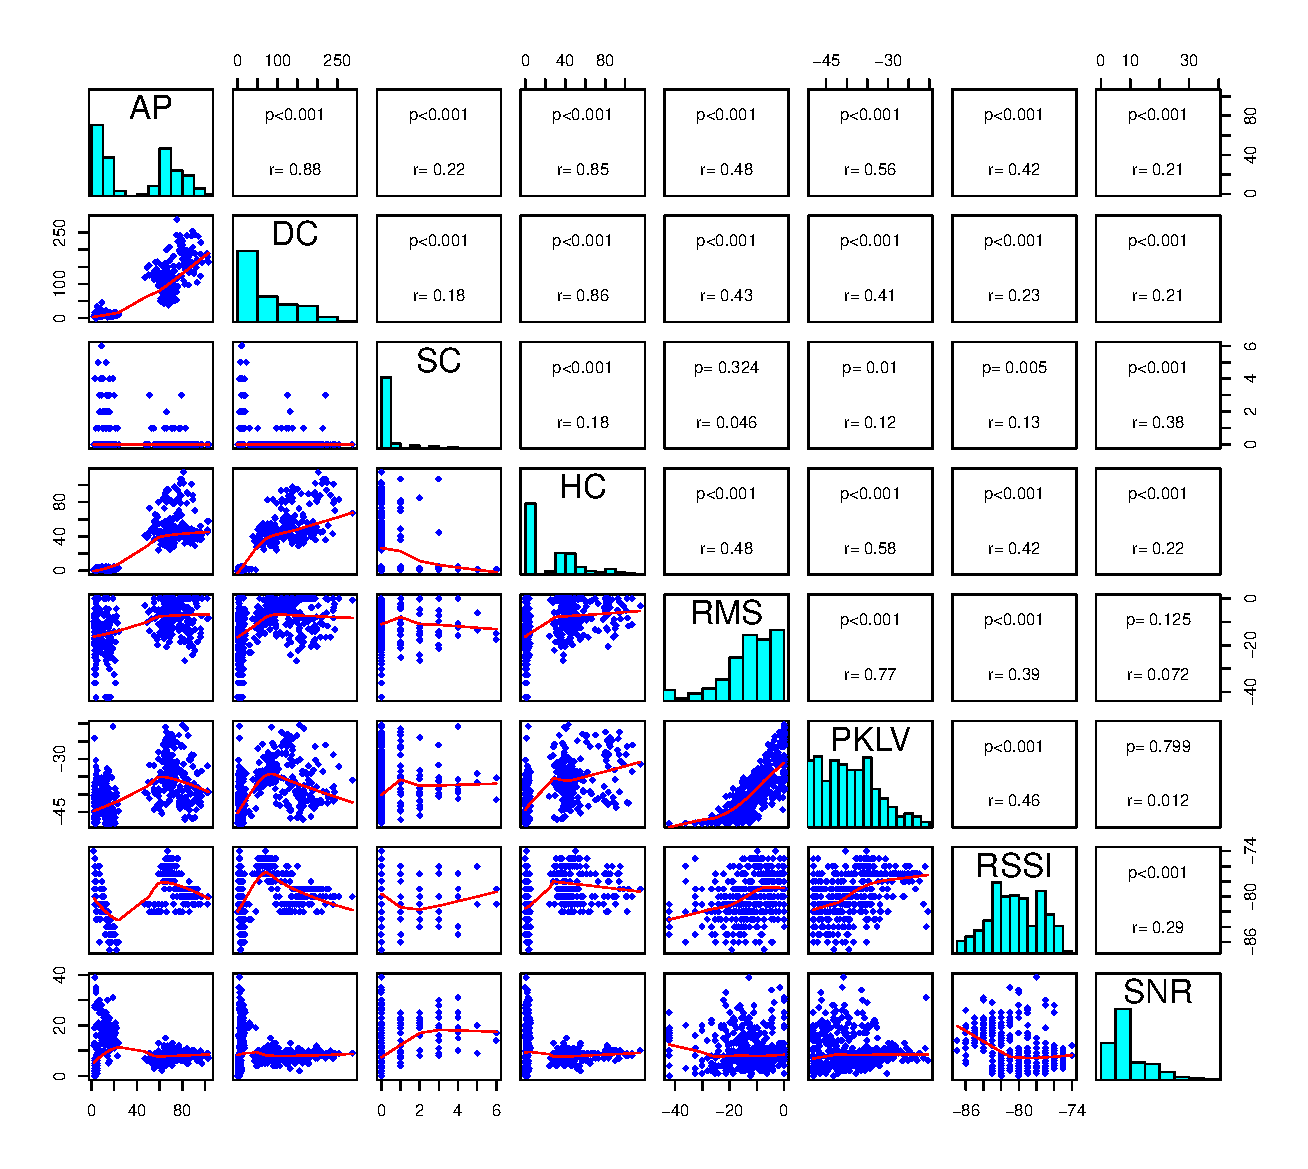
\includegraphics[width=1.3\textwidth]{./img/result/all-result}
		\end{adjustwidth}
		\caption[Scatter plot matrix of all parameters.]
		{Scatter plot matrix showing all parameters correlation of all collected data. The top right shows the correlation coefficient $r$ and the p-value. Along the diagonal are the histograms of each parameter.}
		\label{fig:scatterplot-matrix}
	\end{figure}

	% In the next chapter, we present regression analysis about social level density estimation using all data from four days experiment. The regression analysis tries to estimate the social density estimation using consumer smartphone sensor readings.

	% We predict the head count or device count from other parameters, e.g., \ac{AP}, \ac{RMS}, \ac{PKLV}, and \ac{RSSI}. We do not use \ac{SC} as a predicting variable because speaker count value is almost at zero, which does not give us any meaningful insight, and we do not use \ac{SNR} parameter as well, because we derive signal to noise ratio from probe request packet capture in a laptop, which smartphone cannot capture.

	% Make the datasets available online.
	% Make sure that the data is available publicly, mention the url.

% regression
% \added{
\section{Social Density Prediction} % (fold)
\label{sec:social-density-prediction}
We construct data models so that we are able to predict the level of social density from new data. We use supervised learning techniques using three predictors, namely linear regression, k-Nearest Neighbor (\ac{k-NN}), and Support Vector Machine (\ac{SVM}), so that we can compare which predictor gives optimal model.

We predict the head count or device count from other parameters, e.g., \ac{AP}, \ac{RMS}, \ac{PKLV}, and \ac{RSSI}. We do not use \ac{SC} as a predicting variable because speaker count value is almost at zero, which does not give us any meaningful insight, and we do not use \ac{SNR} parameter as well, because we derive signal to noise ratio from probe request packet capture in a laptop, which smartphone cannot capture. Our dataset contains 459 records.

We validate our model using 10-folds cross-validation, which is a method to assess the performance of a prediction model. The cross-validation technique involves dataset partition into complementary subsets, namely training and testing sets, in which training subsets are for performing the analysis, while testing subsets are for the validation of the resulting model. 10-folds cross-validation divides the dataset to 10 complementary subsets, in which one subset will be the testing set and the other nine subsets are the training set, interchangeably in 10 times.
% }

We use \ac{RMSE} as the metric for cross-validation. In this metric, the optimal model has lower \ac{RMSE} value. The formula of \ac{RMSE} is as follows,
\begin{equation} \label{eq:rmse}
 RMSE=\sqrt { \frac { \sum _{ i=1 }^{ n }{ { \left( { p }_{ i }-{ a }_{ i } \right)  }^{ 2 } }  }{ n }  } 
\end{equation}
where ${ p }_{ i }$ is the predicted value, ${ a }_{ i }$ is the actual value, and $n$ is the number of cases. We implement the analysis using R~\cite{r-team}, presented in \autoref{ch:R-code-listings}.


	\subsection{Linear Regression} % (fold)
	\label{sub:linear_estimator}
	Linear regression is a method of modeling the relationship between a dependent variable and an explanatory (or predicting) variable by fitting a straight line across the data. A condition where there is only one explanatory variable is called simple linear regression, while multiple linear regression involves more than one explanatory variable. The result of linear regression is a linear function (or a model) with the explanatory variables as the parameters.

	To obtain a model with minimal error, we perform an exhaustive search for the best subsets of the predictors for predicting the dependent variable (head or device count) in linear regression. We use \ac{RMSE} of 10-folds cross-validation to select the optimal model using the smallest value. \autoref{r-code-linear-regr}~displays the implementation of linear regression analysis. We implement linear regression in R using \verb|caret| library~\cite{caret}. 
	
	\begin{figure}[H]
		\begin{adjustwidth}{-1cm}{}
		\centering
		\subfloat[head count]{
			\label{fig:tuning-linear-headcount}{
				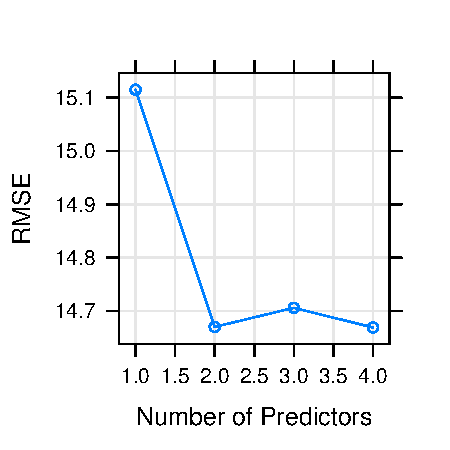
\includegraphics[width=0.65\textwidth]{./img/modeling/linear-regr-hc-small}
			}
		}
		\subfloat[device count]{
			\label{fig:tuning-linear-devicecount}{
				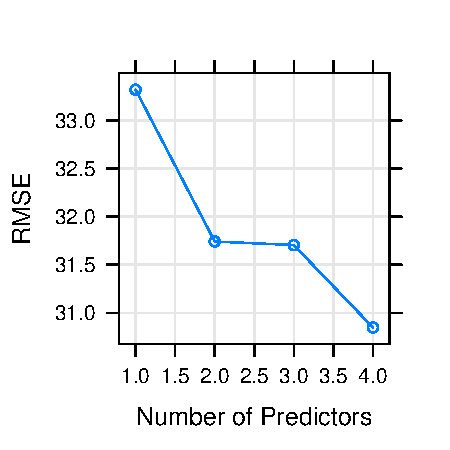
\includegraphics[width=0.65\textwidth]{./img/modeling/linear-regr-dc-small}
			}
		}
		\end{adjustwidth}
		\caption[Tuning linear regression.]
		{Tuning linear regression using best subsets combination for head count (\ref{fig:tuning-linear-headcount}) and device count (\ref{fig:tuning-linear-devicecount}). The result indicates that using all predictors gives the best result, although in head count prediction using two predictors results in nearly the same error.}
		\label{fig:tuning-linear}
	\end{figure}

	\autoref{fig:tuning-linear}~presents the tuning result. For both head count and device count, using all four predictors results in optimal model. In head count prediction, using two predictors ($ap$ and $pklv$) yields in nearly identical \ac{RMSE} as using four predictors. Based on the tuning, we develop a linear model to predict the head count and device count. The linear regression fit to the dataset is depicted in~\autoref{tab:linear-model-hc-dc}.

	
		\begin{table}[h]
		\centering
		\caption[Linear model fit to the dataset]
		{Linear model fit to the dataset with corresponding coefficient for head count and device count model.}
		\label{tab:linear-model-hc-dc}
		\begin{tabular}{rrr}
		\toprule
		\multicolumn{1}{l}{\multirow{2}{*}{Term}} & \multicolumn{2}{c}{Coefficient}                                   \\
		\multicolumn{1}{l}{}                      & \multicolumn{1}{c}{Head count} & \multicolumn{1}{c}{Device count} \\ \midrule
		\verb|Intercept|                          & 54.675 & -367.901 \\
		\verb|ap|                                 & 0.653  & 2.021 \\
		\verb|rms|                                & -0.109 & 1.138 \\
		\verb|pklv|                               & 0.760  & -1.880 \\
		\verb|rssi|                               & 0.329  & -3.656 \\ \bottomrule
		\end{tabular}
		\end{table}
	

	% , using an efficient branch-and-bound algorithm. 

	% predictions and real result, show the graph as well, better using line graph
	% mention what is the training and what is the testing (better using 10 fold cross validation)
	

	% hc ==========================
	% Subset selection object
	% 4 Variables  (and intercept)
	%      Forced in Forced out
	% ap       FALSE      FALSE
	% rms      FALSE      FALSE
	% pklv     FALSE      FALSE
	% rssi     FALSE      FALSE
	% 1 subsets of each size up to 4
	% Selection Algorithm: forward
	%          ap  rms pklv rssi
	% 1  ( 1 ) "*" " " " "  " " 
	% 2  ( 1 ) "*" " " "*"  " " 
	% 3  ( 1 ) "*" " " "*"  "*" 
	% 4  ( 1 ) "*" "*" "*"  "*" 

	% Linear Regression with Stepwise Selection 

	% 459 samples
	%   4 predictor

	% No pre-processing
	% Resampling: Cross-Validated (10 fold, repeated 10 times) 
	% Summary of sample sizes: 414, 413, 412, 412, 412, 413, ... 
	% Resampling results across tuning parameters:

	%   nvmax  RMSE      Rsquared 
	%   1      15.11505  0.7320710
	%   2      14.67019  0.7467084
	%   3      14.70598  0.7455704
	%   4      14.66907  0.7467488

	% RMSE was used to select the optimal model using  the smallest value.
	% The final value used for the model was nvmax = 4. 

	% Call:
	% lm(formula = gt ~ ., data = phone_data_gt)

	% Coefficients:
	% (Intercept)           ap          rms         pklv         rssi  
	%     54.6750       0.6530      -0.1091       0.7603       0.3288 

	% \begin{figure}[h]
	% 	\centering
	% 	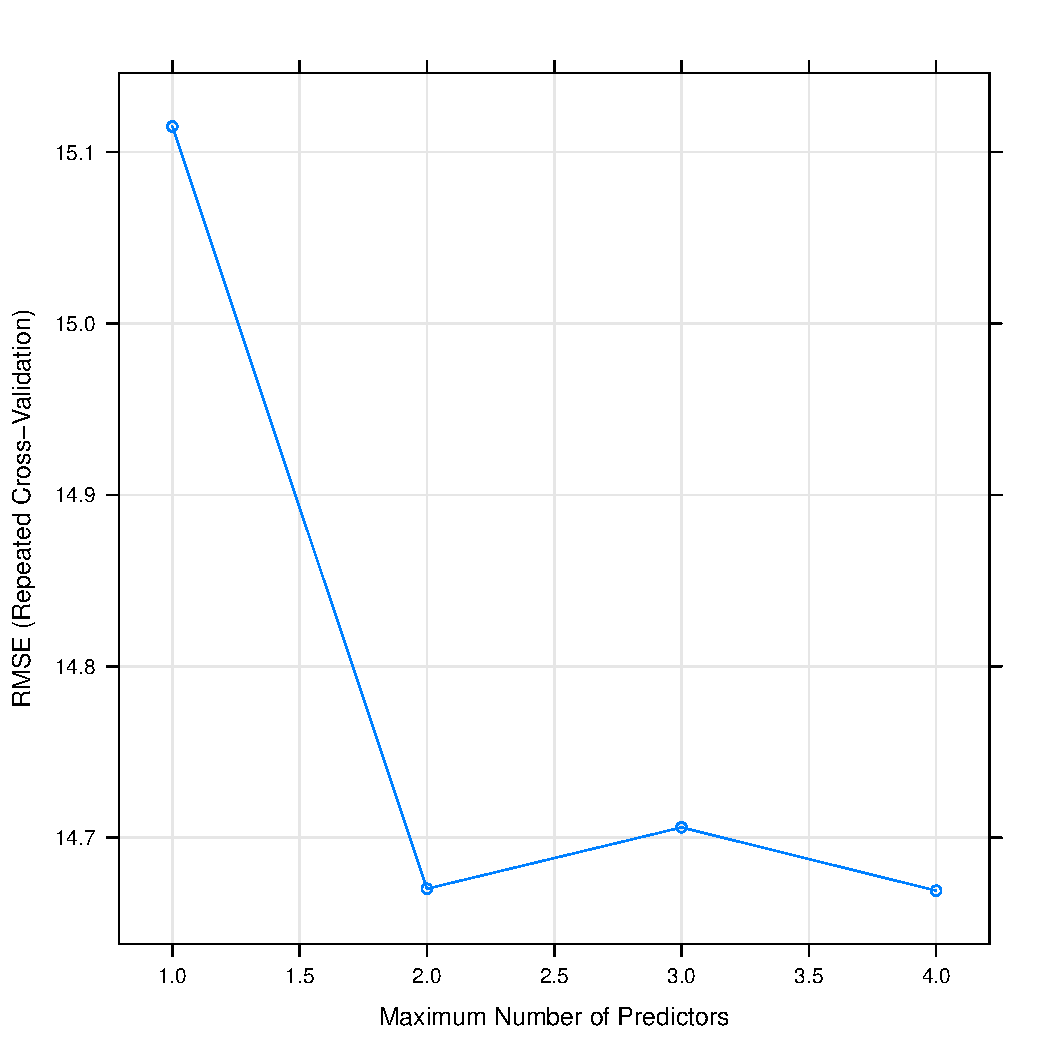
\includegraphics[width=0.9\textwidth]{./img/modeling/linear-regr-hc}
	% 	\caption{Tuning for linear regression.}
	% 	\label{fig:tuning-linear-hc}
	% \end{figure}

	% dc =========================
	% Subset selection object
	% 4 Variables  (and intercept)
	%      Forced in Forced out
	% ap       FALSE      FALSE
	% rms      FALSE      FALSE
	% pklv     FALSE      FALSE
	% rssi     FALSE      FALSE
	% 1 subsets of each size up to 4
	% Selection Algorithm: 'sequential replacement'
	%          ap  rms pklv rssi
	% 1  ( 1 ) "*" " " " "  " " 
	% 2  ( 1 ) "*" " " " "  "*" 
	% 3  ( 1 ) "*" " " "*"  "*" 
	% 4  ( 1 ) "*" "*" "*"  "*" 

	% Linear Regression with Stepwise Selection 

	% 459 samples
	%   4 predictor

	% No pre-processing
	% Resampling: Cross-Validated (10 fold, repeated 10 times) 
	% Summary of sample sizes: 414, 414, 413, 411, 414, 413, ... 
	% Resampling results across tuning parameters:

	%   nvmax  RMSE      Rsquared 
	%   1      33.32081  0.7752300
	%   2      31.74120  0.7979257
	%   3      31.70418  0.7990889
	%   4      30.84697  0.8103420

	% RMSE was used to select the optimal model using  the smallest value.
	% The final value used for the model was nvmax = 4.

	% Call:
	% lm(formula = pr ~ ., data = phone_data_pr)

	% Coefficients:
	% (Intercept)           ap          rms         pklv         rssi  
	%    -367.901        2.021        1.138       -1.880       -3.656 
	% \begin{figure}[h]
	% 	\centering
	% 	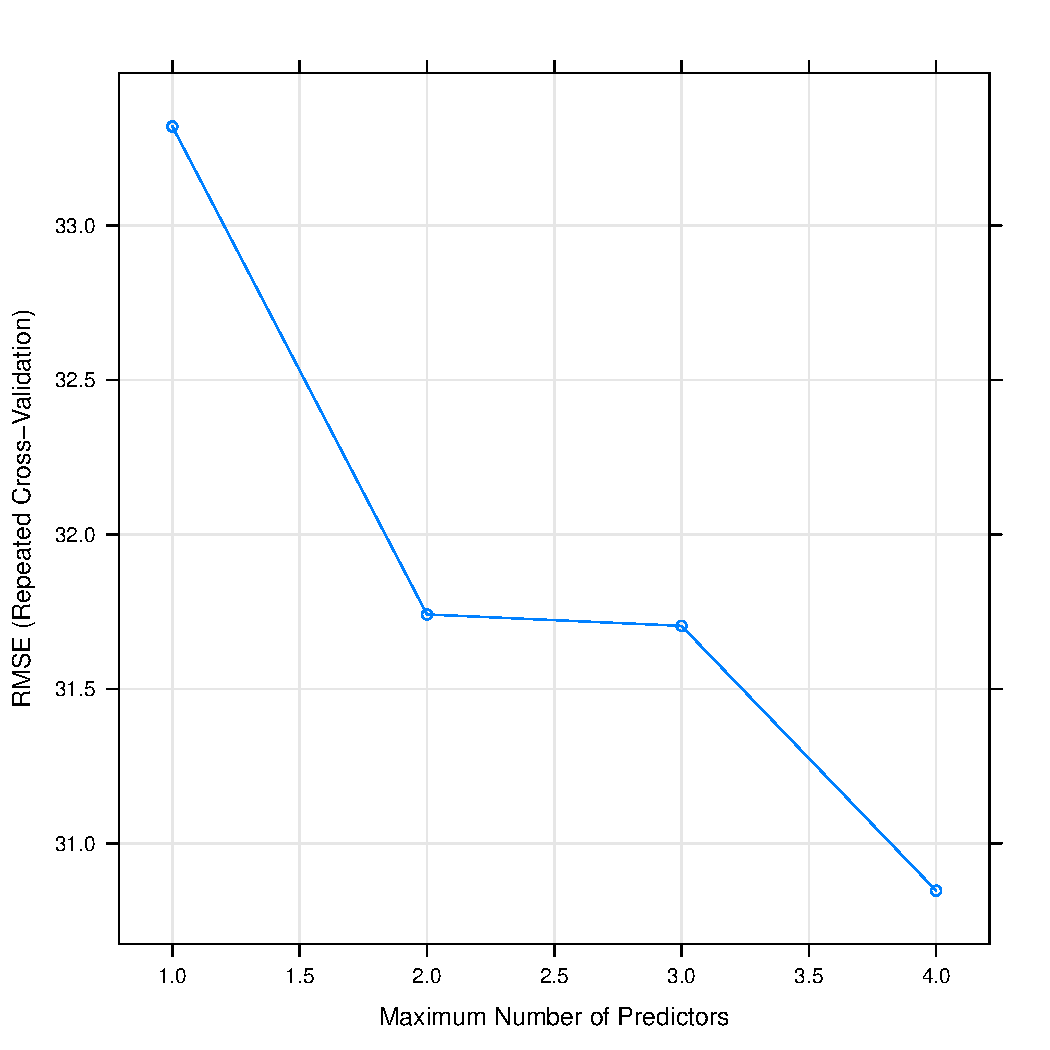
\includegraphics[width=0.9\textwidth]{./img/modeling/linear-regr-dc}
	% 	\caption{Tuning for linear regression.}
	% 	\label{fig:tuning-linear-dc}
	% \end{figure}

	\subsection{k-Nearest Neighbor} % (fold)
	\label{sub:k_nearest_neighbor}
	% subsection k_nearest_neighbor (end)
	% =====================knn===================================
	k-Nearest Neighbor (\ac{k-NN}) is an algorithm that predicts numerical value based on similarity measure using distance function of k-nearest neighbors of the predicted value.
	% Generally, a large $k$ value is more accurate as it uses more neighbors to predict a new value. \ac{k-NN} is applicable for both classification and regression analysis.

	\begin{figure}[H]
		\begin{adjustwidth}{-1cm}{}
		\centering
		\subfloat[head count]{
			\label{fig:tuning-knn-hc}{
				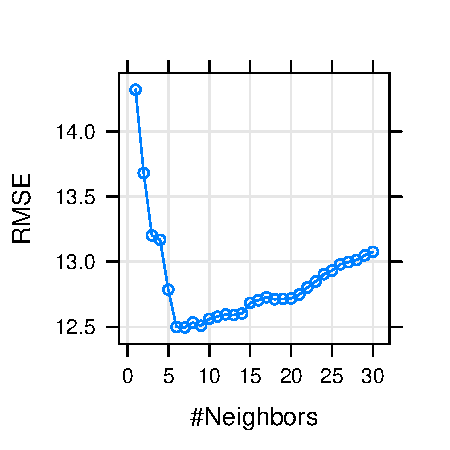
\includegraphics[width=0.65\textwidth]{./img/modeling/knn-hc-small}
			}
		}
		\subfloat[device count]{
			\label{fig:tuning-knn-dc}{
				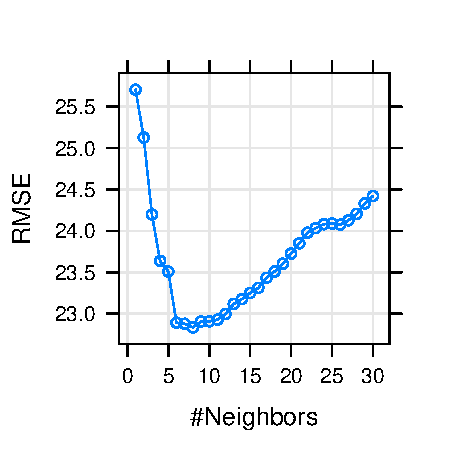
\includegraphics[width=0.65\textwidth]{./img/modeling/knn-dc-small}
			}
		}
		\end{adjustwidth}
		\caption[Tuning \ac{k-NN}.]
		{Tuning \ac{k-NN} using $1 \le k \le 30$ as the tuning parameter (\#Neighbors) for head count (\ref{fig:tuning-knn-hc}) and device count (\ref{fig:tuning-knn-dc}). For both estimation, optimal result is obtained when $5 \le k \le 10$. The optimal result is chosen at $k=7$ (head count) and $k=8$ (device count).}
		\label{fig:tuning-knn}
	\end{figure}

	We train and test \ac{k-NN} regression using $1 \le k \le 30$ as the tuning parameter in R using \verb|caret| library~\cite{caret}. Similar in the linear regression analysis, we evaluate the model using 10-folds cross-validation and we use \ac{RMSE} to select the optimal model with lowest error. \autoref{r-code-knn}~displays the implementation of \ac{k-NN} regression.

	\autoref{fig:tuning-knn}~presents the tuning result.
	% As we can see, the optimal models are obtained when $5 \le k \le 10$.
	According to~\autoref{fig:tuning-knn}, the highest error of both estimation is when $k=1$ and there is an increasing trend of error as $k$ goes up.
	% \added{
		The tuning results indicate that the optimal model for head count estimation is achieved when $k=7$ ($RMSE=12.49515$), while the optimal model for device count estimation is when $k=8$ ($RMSE=22.83321$).
	% }
	% hc ========================================================
	% k-Nearest Neighbors 

	% 459 samples
	%   4 predictor

	% No pre-processing
	% Resampling: Cross-Validated (10 fold, repeated 10 times) 
	% Summary of sample sizes: 414, 413, 412, 412, 412, 413, ... 
	% Resampling results across tuning parameters:

	%   k   RMSE      Rsquared 
	%    1  14.32195  0.7651252
	%    2  13.68100  0.7813994
	%    3  13.20218  0.7946098
	%    4  13.16852  0.7956532
	%    5  12.78561  0.8064473
	%    6  12.49908  0.8149187
	%    7  12.49515  0.8156143
	%    8  12.53433  0.8148571
	%    9  12.50869  0.8159582
	%    ...
	%   30  13.07611  0.7998607

	% RMSE was used to select the optimal model using  the smallest value.
	% The final value used for the model was k = 7. 

	%             Length Class      Mode     
	% learn       2      -none-     list     
	% k           1      -none-     numeric  
	% theDots     0      -none-     list     
	% xNames      4      -none-     character
	% problemType 1      -none-     character
	% tuneValue   1      data.frame list     
	% obsLevels   1      -none-     logical  

	% dc ========================================================
	% k-Nearest Neighbors 

	% 459 samples
	%   4 predictor

	% No pre-processing
	% Resampling: Cross-Validated (10 fold, repeated 10 times) 
	% Summary of sample sizes: 414, 414, 413, 411, 414, 413, ... 
	% Resampling results across tuning parameters:

	%   k   RMSE      Rsquared 
	%    1  25.70729  0.8686436
	%    2  25.12761  0.8746131
	%    3  24.19895  0.8823375
	%    4  23.63810  0.8880587
	%    5  23.50962  0.8894205
	%    6  22.89128  0.8950484
	%    7  22.87820  0.8953308
	%    8  22.83321  0.8958578
	%    9  22.90468  0.8955070
	%   10  22.90716  0.8953828
	%   ...
	%   30  24.42160  0.8851021

	% RMSE was used to select the optimal model using  the smallest value.
	% The final value used for the model was k = 8. 

	%             Length Class      Mode     
	% learn       2      -none-     list     
	% k           1      -none-     numeric  
	% theDots     0      -none-     list     
	% xNames      4      -none-     character
	% problemType 1      -none-     character
	% tuneValue   1      data.frame list     
	% obsLevels   1      -none-     logical 


	\subsection{Support Vector Machine} % (fold)
	\label{sub:support_vector_machine}
	% subsection support_vector_machine (end)
	% =======================svm=============================================
	Support Vector Machine (\ac{SVM}) is an estimator that works by constructing support vectors (hyperplanes) that separate the data according to a certain threshold. Most of the time, a kernel, a set of mathematical functions, is used to
	define the decision boundary.
	% \ac{SVM} is also implementable for both classification and regression analysis.

	We implement \ac{SVM} to predict quantities using radial kernel with $cost$ and $\epsilon$ as the tuning parameters.
	$cost$ parameter is used to define the width of the hyperplane, while $\epsilon$ is used to determine how non-linear the decision boundary is.
	As used in \ac{k-NN}, we validate the model using 10-folds cross-validation.
	We use grid search method to tune the optimal parameters. It tries to find the best combination of the two parameters in certain range of search.
	We implement the analysis in R with \verb|e1071| library~\cite{e1071}. \autoref{r-code-svm}~displays the implementation of \ac{SVM} prediction.

	\begin{figure}[H]
		\begin{adjustwidth}{-3cm}{}
		\centering
		\subfloat[head count]{
			\label{fig:tuning-svm-hc}{
				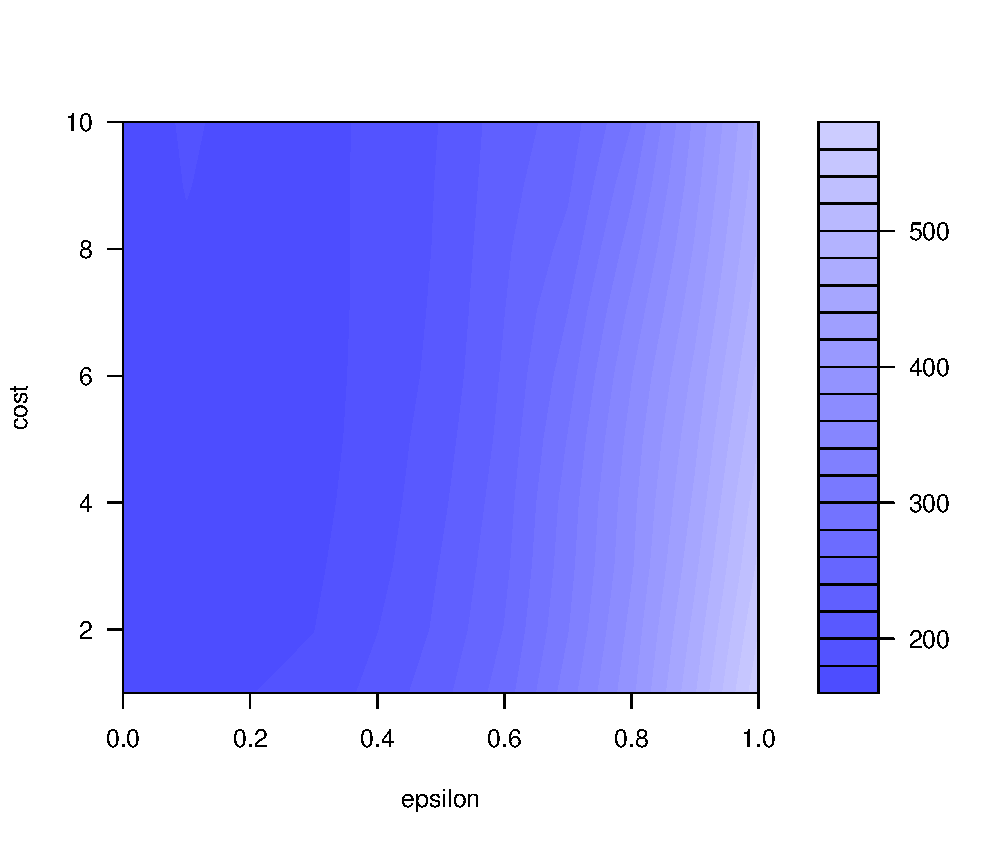
\includegraphics[width=0.65\textwidth]{./img/modeling/svm-hc}
			}
		}
		\subfloat[device count]{
			\label{fig:tuning-svm-dc}{
				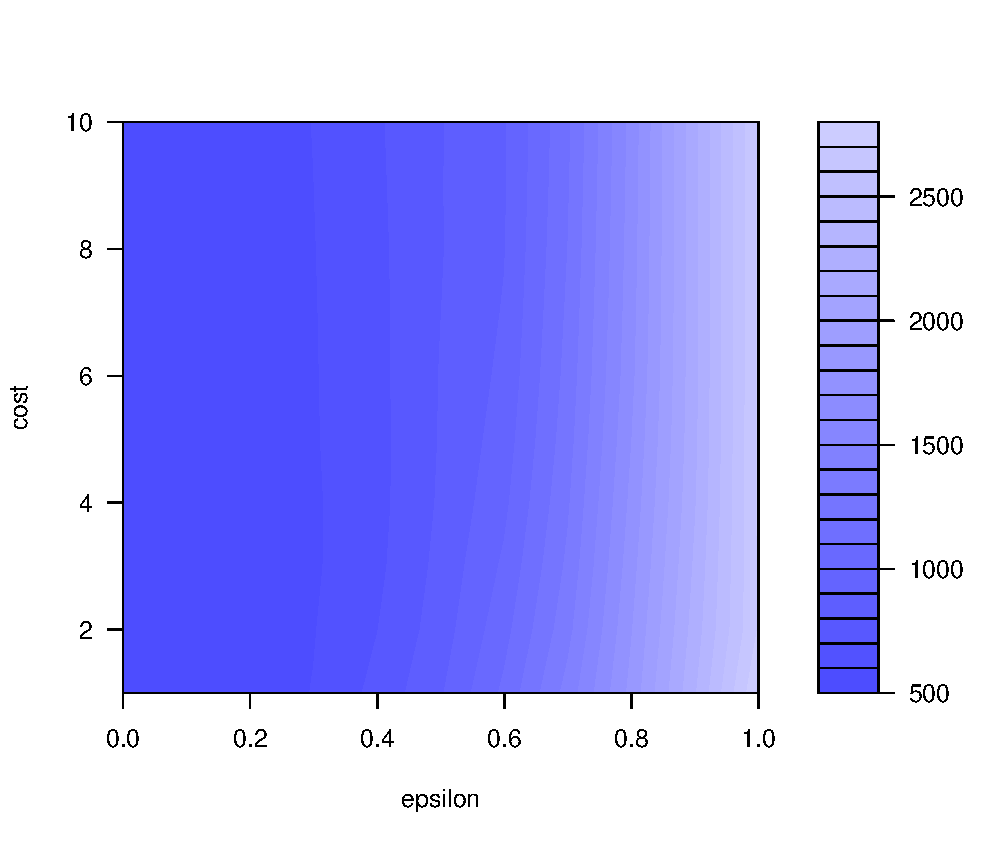
\includegraphics[width=0.65\textwidth]{./img/modeling/svm-dc}
			}
		}
		\end{adjustwidth}
		\caption[Tuning \ac{SVM}.]
		{Tuning \ac{SVM} using grid search technique. Two tuning parameters $\epsilon$ and $cost$ are represented in $x$ and $y$ axis, while the performance (measured using \ac{MSE}) is represented in color. More optimal model is indicated by darker color, i.e., lower \ac{MSE} (see color bar).}
		\label{fig:tuning-svm}
	\end{figure}

	We present the result of \ac{SVM} regression tuning in~\autoref{fig:tuning-svm}.
	% \added{
	We focus the grid search within $0 \le cost \le 10$ and $0 \le \epsilon \le 1$ to reduce the computational time. Moreover, our previous grid search, which involves wider area, indicates that \ac{SVM} performs better within that area.
	% }

	We measure the performance of the \ac{SVM} using mean squared error (\ac{MSE}), in which best result has lower \ac{MSE}. The best performance for head count prediction is at 171.1065 with $\epsilon=0$ and $cost=3$, while for device count prediction is at 514.226 with $\epsilon=0$ and $cost=1$. We can also see a trend of increasing \ac{MSE} as the $epsilon$ increases.
	% hc============
	% Parameter tuning of 'svm':

	% - sampling method: 10-folds cross validation 

	% - best parameters:
	%  epsilon cost
	%        0    3

	% - best performance: 171.1065 


	% dc============
	% Parameter tuning of 'svm':

	% - sampling method: 10-folds cross validation 

	% - best parameters:
	%  epsilon cost
	%        0    1

	% - best performance: 514.226 

To summarize the regression analysis and to interpret the result, we use another approach to calculate the error, which has more intuitive interpretation. We use residual error, which can be formulated as

\begin{equation}\label{eq:residual-error}
	\overline { error } =\frac { 1 }{ n } \left( \sum _{ i=1 }^{ n }{ \left| { p }_{ i }-{ a }_{ i } \right|  }  \right) 
\end{equation}

\noindent
As formulated in the equation, residual error shows the mean of the difference between predicted and actual value. Using the optimum model of each regression technique, we perform another 10-fold cross validation to obtain residual error measurement. The optimal model has a residual error closer to zero.

\begin{table}[h]
\centering
\caption[Summary of regression analysis]
{Summary of regression analysis showing the range of the data and the residual error of each regression method.}
\label{tab:regression-summary}
\begin{tabular}{llllll}
\toprule
                   & \multicolumn{2}{c}{Value Range}                         & \multicolumn{3}{c}{Residual Error}                                                        \\
                   & \multicolumn{1}{c}{Min} & \multicolumn{1}{c}{Max} & \multicolumn{1}{c}{Linear} & \multicolumn{1}{c}{k-NN} & \multicolumn{1}{c}{SVM} \\ \midrule
Head count estimation   & 0                       & 115                     & 9.89                                  & 7.05                    & 7.06                    \\
Device count estimation & 0                       & 288                     & 23.81                                 & 13.14                   & 13.34                  \\ \bottomrule
\end{tabular}
\end{table}

\autoref{tab:regression-summary}~presents the summary of the regression analysis. \ac{k-NN} and \ac{SVM} have better performance than the linear regression. \ac{k-NN} and \ac{SVM} do not have much difference of error for both head count and device count estimation. Device count estimation has wider value range and error compared to head count estimation.

% Plot the prediction graph in each cross validation round, then combined.
% Explain the result in percentage as well, instead of manual count. -> for the error in the modeling.
% plot the graph of head count (real vs predicted) vs parameters (ap count, or anything else)
% present the evaluation in people count and also percentage

%*****************************************
%*****************************************
%*****************************************
%*****************************************
%*****************************************

%!TEX root = ../thesis-guntur.tex
%************************************************
\chapter{Regression Analysis and Discussion}
\label{ch:regression-and-discussion} % $\mathbb{ZNR}$
%************************************************
In this chapter, we firstly present regression analysis to construct a data model for social density estimation in the future. Then we discuss and interpret the result of the experiments.
% In this chapter we look at to what extend these questions have been answered, what problems arose from answering them and what future directions this work can go in.

\section{Regression Analysis} % (fold)
\label{sec:regression_analysis}
We perform regression analysis to the dataset so that we can establish a data model that enables us to predict the level of social density using sensor readings. We decide to use regression analysis as this analysis gives quantitative result, i.e., numbers. On the other hand, another statistical analysis, named classification, yields discrete result, i.e., classes, which is not preferable.

We predict the level of social density by means of proxies, namely the head count and device count. We predict the head count or device count from \ac{AP} count, \ac{RMS}, \ac{PKLV}, and \ac{RSSI} value. Our dataset contains 459 records.

We use linear and non-linear regression analysis, which are validated using 10-folds cross-validation. Cross-validation is a method to assess how the regression analysis results will vary across different datasets. Cross-validation technique involves dataset partition into complementary subsets, namely training and testing sets, in which training subsets are for performing the analysis, while testing subsets are for the validation of the resulting model. 10-folds cross-validation divides the dataset to 10 complementary subsets, in which one subset will be the testing set and the other nine subsets are the training set, interchangeably in 10 times.

We use \ac{RMSE} as the metric for cross-validation. In this metrics, optimal model has lower \ac{RMSE} value. The formula of \ac{RMSE} is as follows,

\begin{equation} \label{eq:rmse}
 RMSE=\sqrt { \frac { \sum _{ i=1 }^{ n }{ { \left( { p }_{ i }-{ a }_{ i } \right)  }^{ 2 } }  }{ n }  } 
\end{equation}

where ${ p }_{ i }$ is the predicted value and ${ a }_{ i }$ is the actual value. We implement the analysis using R~\cite{r-team}, presented in \autoref{ch:R-code-listings}.

% \begin{figure}[h]
% 	\centering
% 	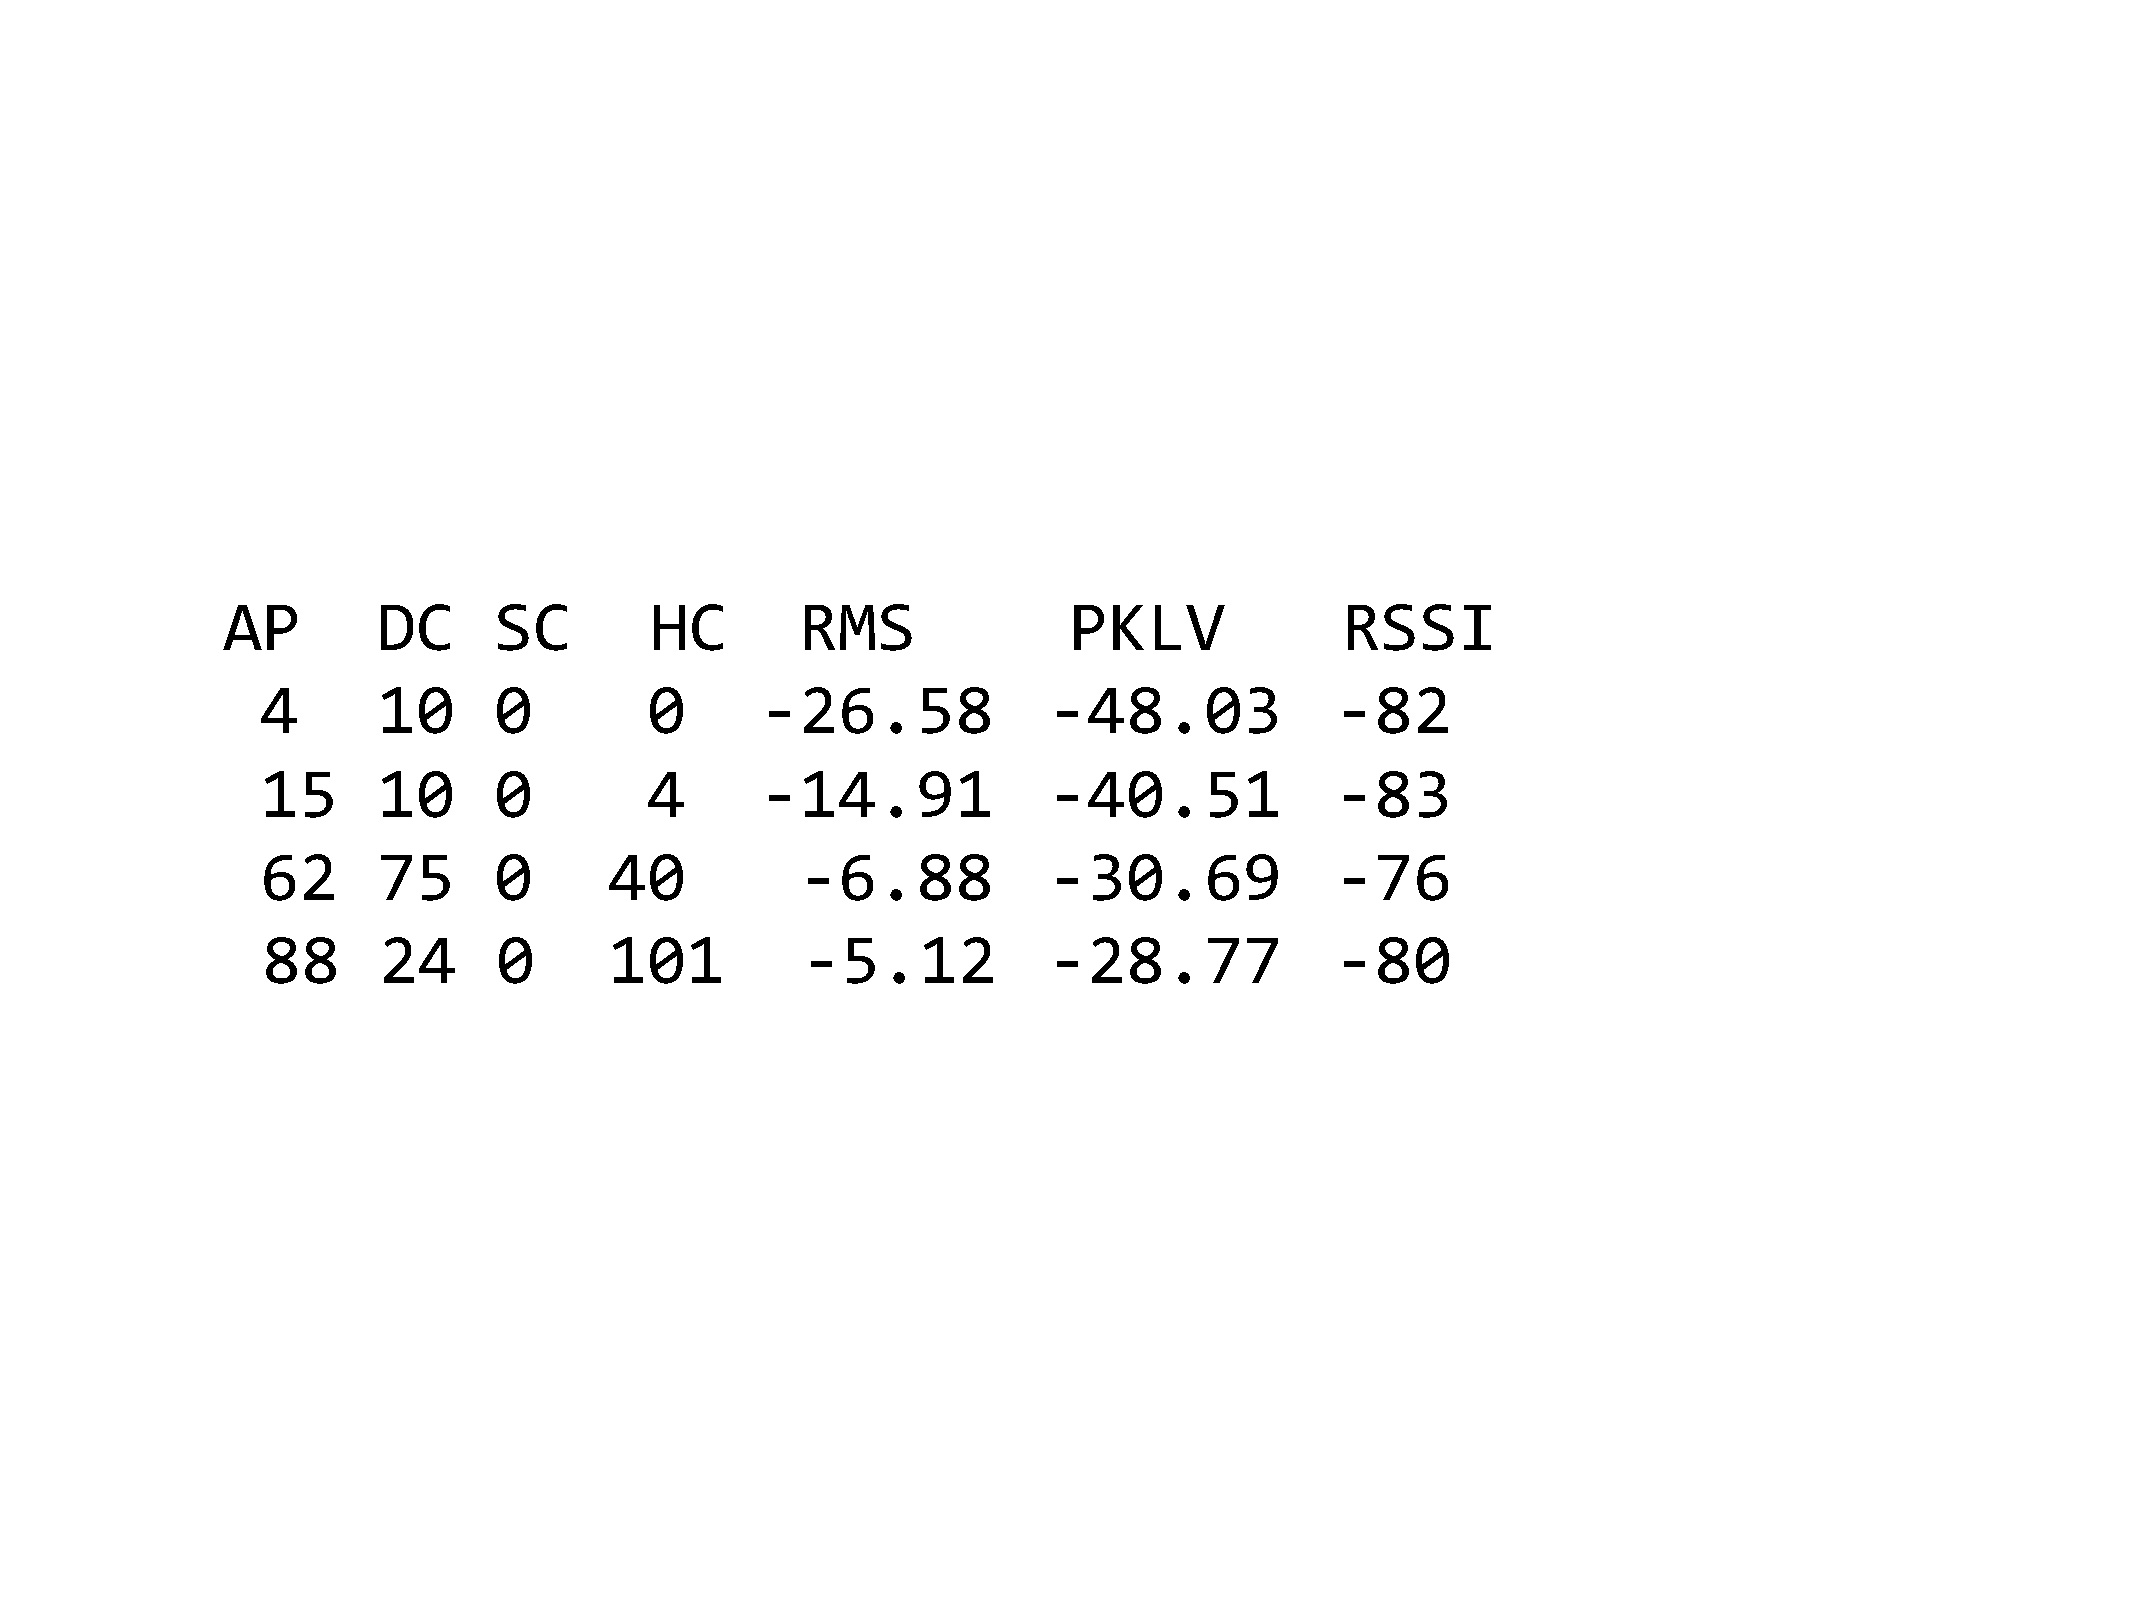
\includegraphics[width=0.7\textwidth]{./img/sensor-readings}
% 	\caption{Example of sensor readings.}
% 	\label{fig:scatterplot-matrix}
% \end{figure}

	\subsection{Linear Method for Regression} % (fold)
	\label{sub:linear_estimator}
	Linear regression is a method of modeling the relationship between a dependent variable and an explanatory (or predicting) variable by fitting a straight line across the data. A condition where there is only one explanatory variable is called simple linear regression, while multiple linear regression involves more than one explanatory variable. The result of linear regression is a linear function (or a model) with the explanatory variables as the parameters.

	To obtain a model with minimal error, we perform an exhaustive search for the best subsets of the predictors for predicting the dependent variable (head or device count) in linear regression. We use \ac{RMSE} of 10-folds cross-validation to select the optimal model using the smallest value. \autoref{r-code-linear-regr}~displays the implementation of linear regression analysis. We implement linear regression using stepwise selection in R using \verb|caret|\footnote{\url{http://topepo.github.io/caret/index.html}} library.
	
	\begin{figure}[h]
		\begin{adjustwidth}{-1cm}{}
		\centering
		\subfloat[head count]{
			\label{fig:tuning-linear-headcount}{
				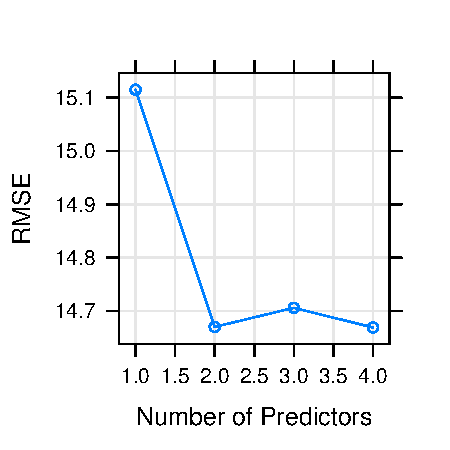
\includegraphics[width=0.65\textwidth]{./img/modeling/linear-regr-hc-small}
			}
		}
		\subfloat[device count]{
			\label{fig:tuning-linear-devicecount}{
				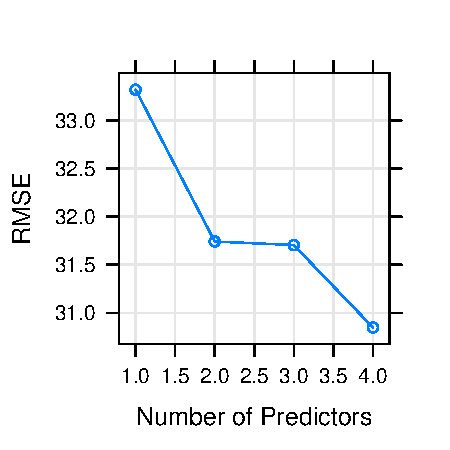
\includegraphics[width=0.65\textwidth]{./img/modeling/linear-regr-dc-small}
			}
		}
		\end{adjustwidth}
		\caption{Tuning linear regression using best subsets combination for head count (\ref{fig:tuning-linear-headcount}) and device count (\ref{fig:tuning-linear-devicecount}). The result indicates that using all predictors gives the best result, although in head count prediction using two predictors results in nearly the same error.}
		\label{fig:tuning-linear}
	\end{figure}

	\autoref{fig:tuning-linear}~presents the tuning result. For both head count and device count, using all four predictors results in optimal model. In head count prediction, using two predictors ($ap$ and $pklv$) yields in nearly identical \ac{RMSE} as using four predictors. Based on the tuning, we develop a linear model to predict the head count and device count. The linear model for head count prediction is 
	\begin{equation}
		hc=54.6750+0.6530ap-0.1091rms+0.7603pklv+0.3288rssi
	\end{equation}
	while the linear model for device count is 
	\begin{equation}
		dc=-367.901+2.021ap+1.138rms-1.880pklv-3.656rssi
	\end{equation}
	where $ap$, $rms$, $pklv$, and $rssi$ represent \ac{AP} count, \ac{RMS} and \ac{PKLV} of ambient noise recording, and \ac{RSSI} of scanned \ac{AP} respectively.
	% , using an efficient branch-and-bound algorithm. 

	% predictions and real result, show the graph as well, better using line graph
	% mention what is the training and what is the testing (better using 10 fold cross validation)
	

	% hc ==========================
	% Subset selection object
	% 4 Variables  (and intercept)
	%      Forced in Forced out
	% ap       FALSE      FALSE
	% rms      FALSE      FALSE
	% pklv     FALSE      FALSE
	% rssi     FALSE      FALSE
	% 1 subsets of each size up to 4
	% Selection Algorithm: forward
	%          ap  rms pklv rssi
	% 1  ( 1 ) "*" " " " "  " " 
	% 2  ( 1 ) "*" " " "*"  " " 
	% 3  ( 1 ) "*" " " "*"  "*" 
	% 4  ( 1 ) "*" "*" "*"  "*" 

	% Linear Regression with Stepwise Selection 

	% 459 samples
	%   4 predictor

	% No pre-processing
	% Resampling: Cross-Validated (10 fold, repeated 10 times) 
	% Summary of sample sizes: 414, 413, 412, 412, 412, 413, ... 
	% Resampling results across tuning parameters:

	%   nvmax  RMSE      Rsquared 
	%   1      15.11505  0.7320710
	%   2      14.67019  0.7467084
	%   3      14.70598  0.7455704
	%   4      14.66907  0.7467488

	% RMSE was used to select the optimal model using  the smallest value.
	% The final value used for the model was nvmax = 4. 

	% Call:
	% lm(formula = gt ~ ., data = phone_data_gt)

	% Coefficients:
	% (Intercept)           ap          rms         pklv         rssi  
	%     54.6750       0.6530      -0.1091       0.7603       0.3288 

	% \begin{figure}[h]
	% 	\centering
	% 	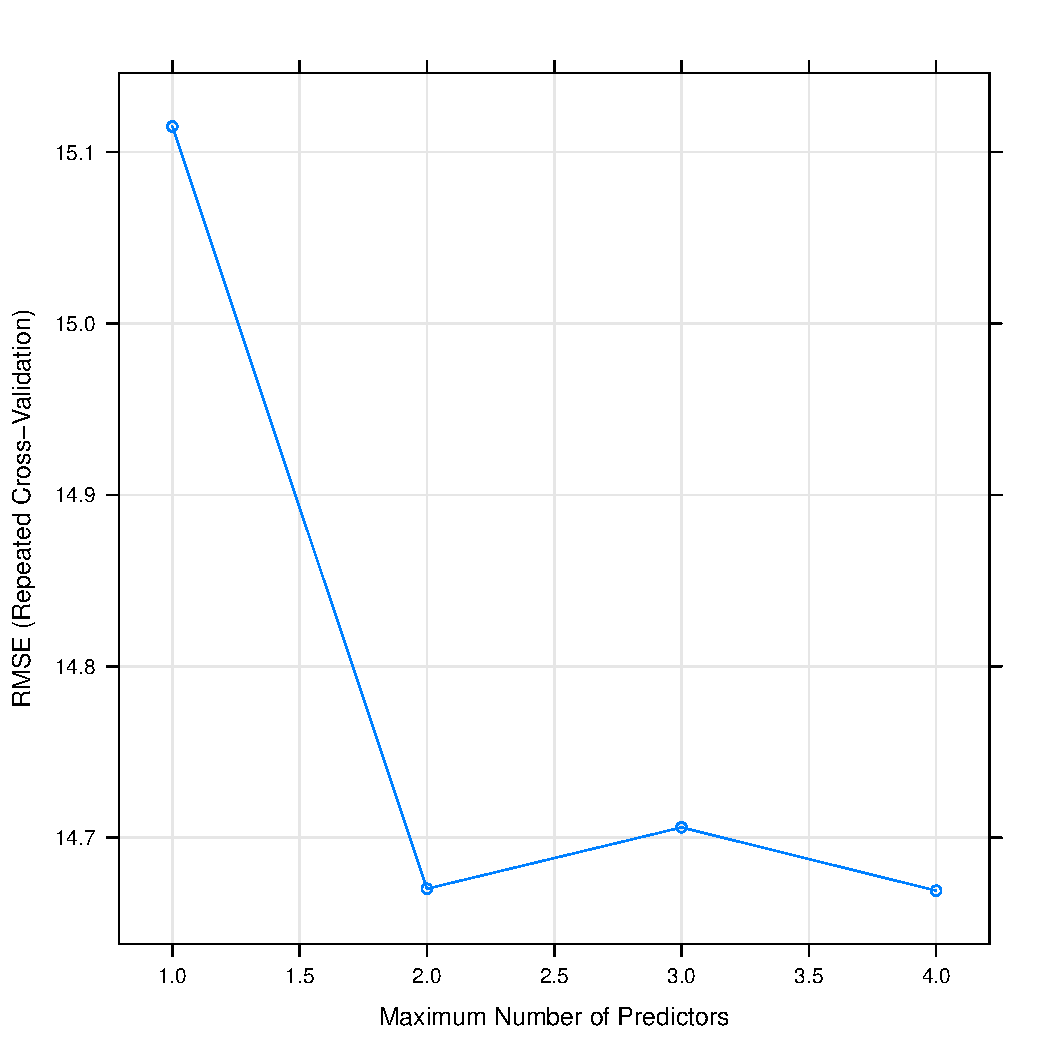
\includegraphics[width=0.9\textwidth]{./img/modeling/linear-regr-hc}
	% 	\caption{Tuning for linear regression.}
	% 	\label{fig:tuning-linear-hc}
	% \end{figure}

	% dc =========================
	% Subset selection object
	% 4 Variables  (and intercept)
	%      Forced in Forced out
	% ap       FALSE      FALSE
	% rms      FALSE      FALSE
	% pklv     FALSE      FALSE
	% rssi     FALSE      FALSE
	% 1 subsets of each size up to 4
	% Selection Algorithm: 'sequential replacement'
	%          ap  rms pklv rssi
	% 1  ( 1 ) "*" " " " "  " " 
	% 2  ( 1 ) "*" " " " "  "*" 
	% 3  ( 1 ) "*" " " "*"  "*" 
	% 4  ( 1 ) "*" "*" "*"  "*" 

	% Linear Regression with Stepwise Selection 

	% 459 samples
	%   4 predictor

	% No pre-processing
	% Resampling: Cross-Validated (10 fold, repeated 10 times) 
	% Summary of sample sizes: 414, 414, 413, 411, 414, 413, ... 
	% Resampling results across tuning parameters:

	%   nvmax  RMSE      Rsquared 
	%   1      33.32081  0.7752300
	%   2      31.74120  0.7979257
	%   3      31.70418  0.7990889
	%   4      30.84697  0.8103420

	% RMSE was used to select the optimal model using  the smallest value.
	% The final value used for the model was nvmax = 4.

	% Call:
	% lm(formula = pr ~ ., data = phone_data_pr)

	% Coefficients:
	% (Intercept)           ap          rms         pklv         rssi  
	%    -367.901        2.021        1.138       -1.880       -3.656 
	% \begin{figure}[h]
	% 	\centering
	% 	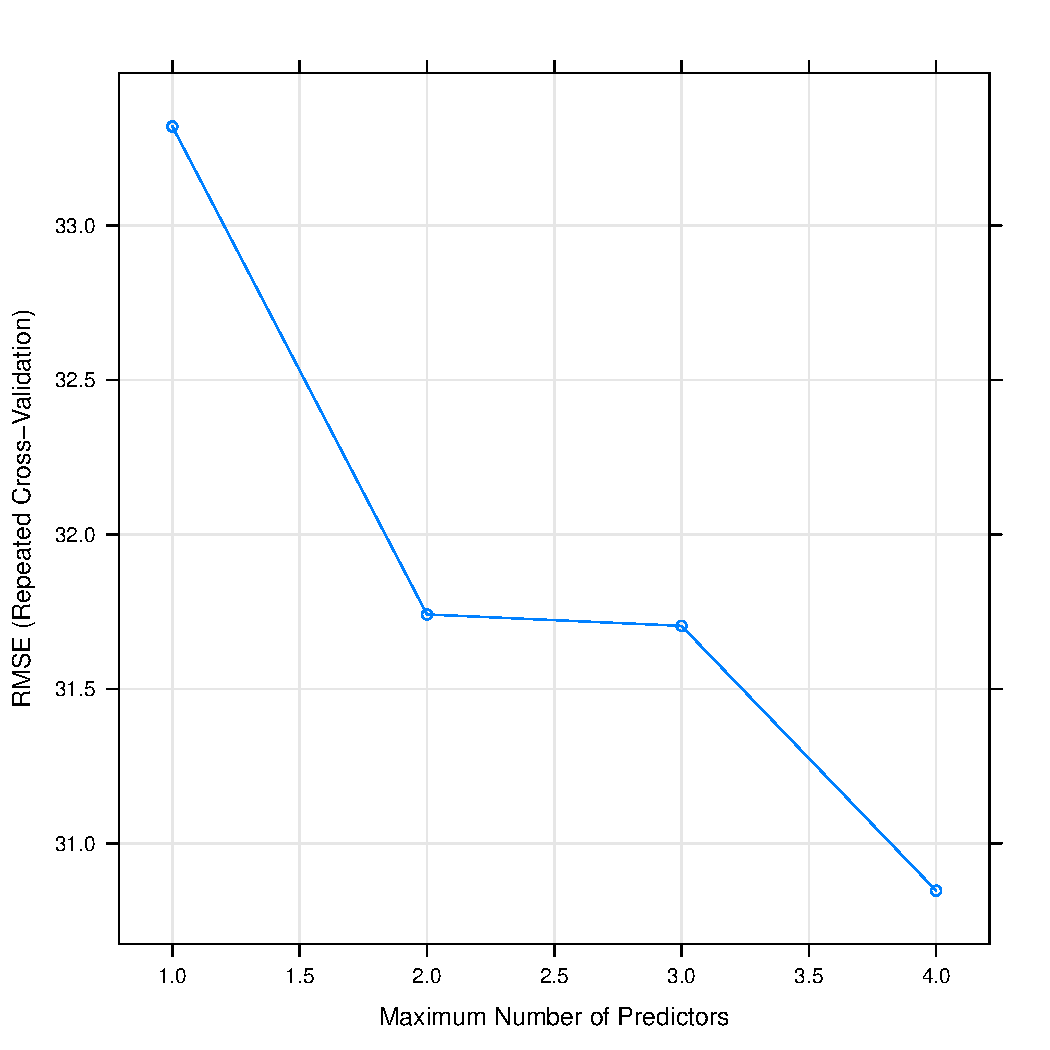
\includegraphics[width=0.9\textwidth]{./img/modeling/linear-regr-dc}
	% 	\caption{Tuning for linear regression.}
	% 	\label{fig:tuning-linear-dc}
	% \end{figure}

	\subsection{Non-Linear Method for Regression} % (fold)
	\label{sub:non_linear_estimator}
	We use \ac{k-NN} and \ac{SVM} as non-linear methods for regression. We tune the parameters of non-linear regression method to obtain the optimal model as well.

	% =====================knn===================================
	\ac{k-NN} is an algorithm that predicts numerical value based on similarity measure using distance function, e.g., euclidean, manhattan, or minkowski, of k-nearest neighbors of the predicted value. Generally, a large $k$ value is more accurate as it uses more neighbors to predict a new value. \ac{k-NN} is applicable for both classification and regression analysis.

	\begin{figure}[h]
		\begin{adjustwidth}{-1cm}{}
		\centering
		\subfloat[head count]{
			\label{fig:tuning-knn-hc}{
				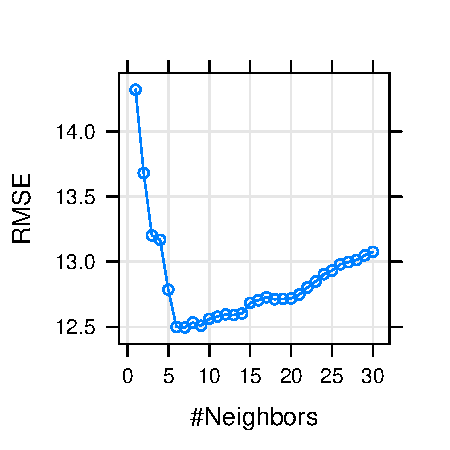
\includegraphics[width=0.65\textwidth]{./img/modeling/knn-hc-small}
			}
		}
		\subfloat[device count]{
			\label{fig:tuning-knn-dc}{
				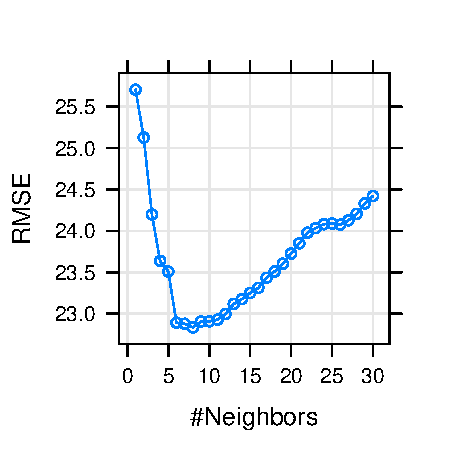
\includegraphics[width=0.65\textwidth]{./img/modeling/knn-dc-small}
			}
		}
		\end{adjustwidth}
		\caption{Tuning \ac{k-NN} using $1 \le k \le 30$ as the tuning parameter (\#Neighbors) for head count (\ref{fig:tuning-knn-hc}) and device count (\ref{fig:tuning-knn-dc}). For both estimation, optimal result is obtained when $5 \le k \le 10$. The optimal result is chosen at $k=7$ (head count) and $k=8$ (device count).}
		\label{fig:tuning-knn}
	\end{figure}

	We train and test \ac{k-NN} regression using $1 \le k \le 30$ as the tuning parameter in R using \verb|caret|\footnote{\url{http://topepo.github.io/caret/index.html}} library. Like the linear regression analysis, we evaluate the model using 10-folds cross-validation and we use \ac{RMSE} to select the optimal model with lowest error. \autoref{r-code-knn}~displays the implementation of \ac{k-NN} regression.

	\autoref{fig:tuning-knn}~presents the tuning result. As we can see, the optimal models are obtained when $5 \le k \le 10$. According to~\autoref{fig:tuning-knn}, the highest error of both estimation is when $k=1$ and there is a increasing trend of error as $k$ goes up. We select the optimal model for head count and device count estimation when $k=7$ ($RMSE=12.49515$) and $k=8$ ($RMSE=22.83321$), respectively.
	% hc ========================================================
	% k-Nearest Neighbors 

	% 459 samples
	%   4 predictor

	% No pre-processing
	% Resampling: Cross-Validated (10 fold, repeated 10 times) 
	% Summary of sample sizes: 414, 413, 412, 412, 412, 413, ... 
	% Resampling results across tuning parameters:

	%   k   RMSE      Rsquared 
	%    1  14.32195  0.7651252
	%    2  13.68100  0.7813994
	%    3  13.20218  0.7946098
	%    4  13.16852  0.7956532
	%    5  12.78561  0.8064473
	%    6  12.49908  0.8149187
	%    7  12.49515  0.8156143
	%    8  12.53433  0.8148571
	%    9  12.50869  0.8159582
	%    ...
	%   30  13.07611  0.7998607

	% RMSE was used to select the optimal model using  the smallest value.
	% The final value used for the model was k = 7. 

	%             Length Class      Mode     
	% learn       2      -none-     list     
	% k           1      -none-     numeric  
	% theDots     0      -none-     list     
	% xNames      4      -none-     character
	% problemType 1      -none-     character
	% tuneValue   1      data.frame list     
	% obsLevels   1      -none-     logical  

	% dc ========================================================
	% k-Nearest Neighbors 

	% 459 samples
	%   4 predictor

	% No pre-processing
	% Resampling: Cross-Validated (10 fold, repeated 10 times) 
	% Summary of sample sizes: 414, 414, 413, 411, 414, 413, ... 
	% Resampling results across tuning parameters:

	%   k   RMSE      Rsquared 
	%    1  25.70729  0.8686436
	%    2  25.12761  0.8746131
	%    3  24.19895  0.8823375
	%    4  23.63810  0.8880587
	%    5  23.50962  0.8894205
	%    6  22.89128  0.8950484
	%    7  22.87820  0.8953308
	%    8  22.83321  0.8958578
	%    9  22.90468  0.8955070
	%   10  22.90716  0.8953828
	%   ...
	%   30  24.42160  0.8851021

	% RMSE was used to select the optimal model using  the smallest value.
	% The final value used for the model was k = 8. 

	%             Length Class      Mode     
	% learn       2      -none-     list     
	% k           1      -none-     numeric  
	% theDots     0      -none-     list     
	% xNames      4      -none-     character
	% problemType 1      -none-     character
	% tuneValue   1      data.frame list     
	% obsLevels   1      -none-     logical 


	% =======================svm=============================================
	\ac{SVM} is an estimator that works by constructing support vectors (hyperplanes) that separate data according to a certain threshold. Most of the time, kernels, a set of mathematical functions, are used to remap the input data so that the data can be separated using a straight line instead of a complex curve. \ac{SVM} is also implementable for both classification and regression analysis.

	We implement \ac{SVM} regression using radial kernel along with $cost$ and $\epsilon$ as the tuning parameters. $cost$ and $\epsilon$ are used to apply a penalty to a prediction where the data are not correctly predicted. As used in \ac{k-NN}, we validate the model using 10-folds cross-validation. We implement the analysis in R with \verb|e1071| library\footnote{\url{https://cran.r-project.org/web/packages/e1071/index.html}}. \autoref{r-code-svm}~displays the implementation of \ac{SVM} regression.

	\begin{figure}[h]
		\begin{adjustwidth}{-1cm}{}
		\centering
		\subfloat[head count]{
			\label{fig:tuning-svm-hc}{
				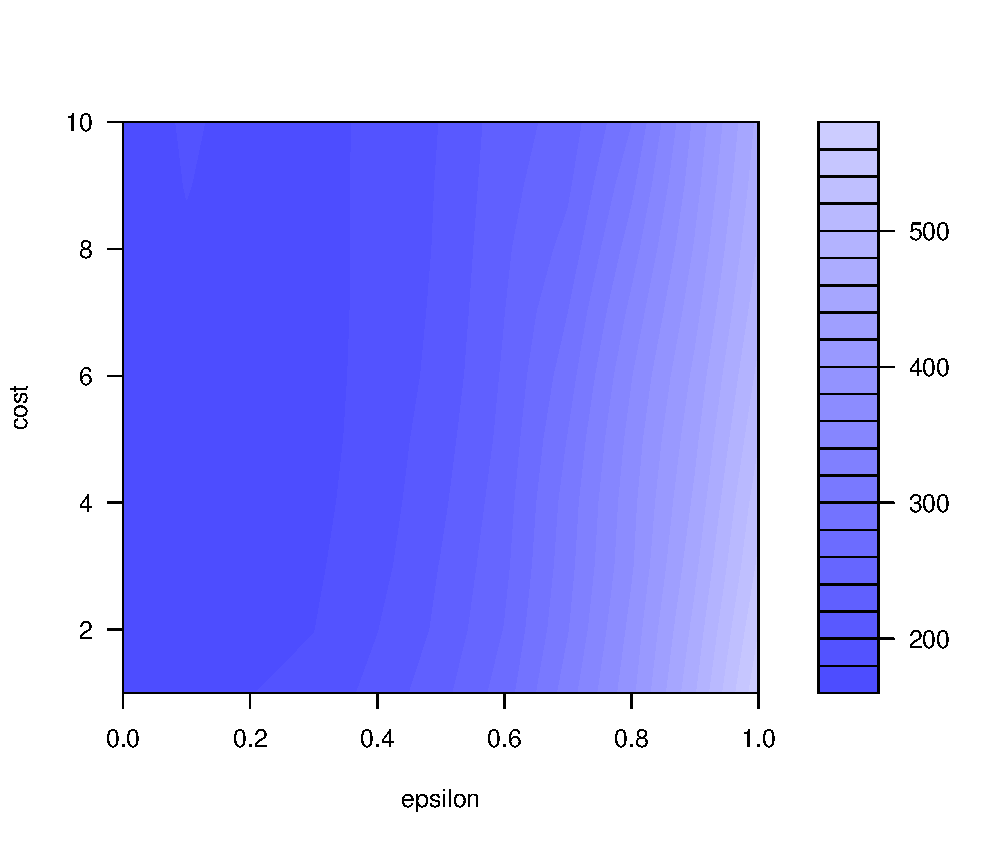
\includegraphics[width=0.65\textwidth]{./img/modeling/svm-hc}
			}
		}
		\subfloat[device count]{
			\label{fig:tuning-svm-dc}{
				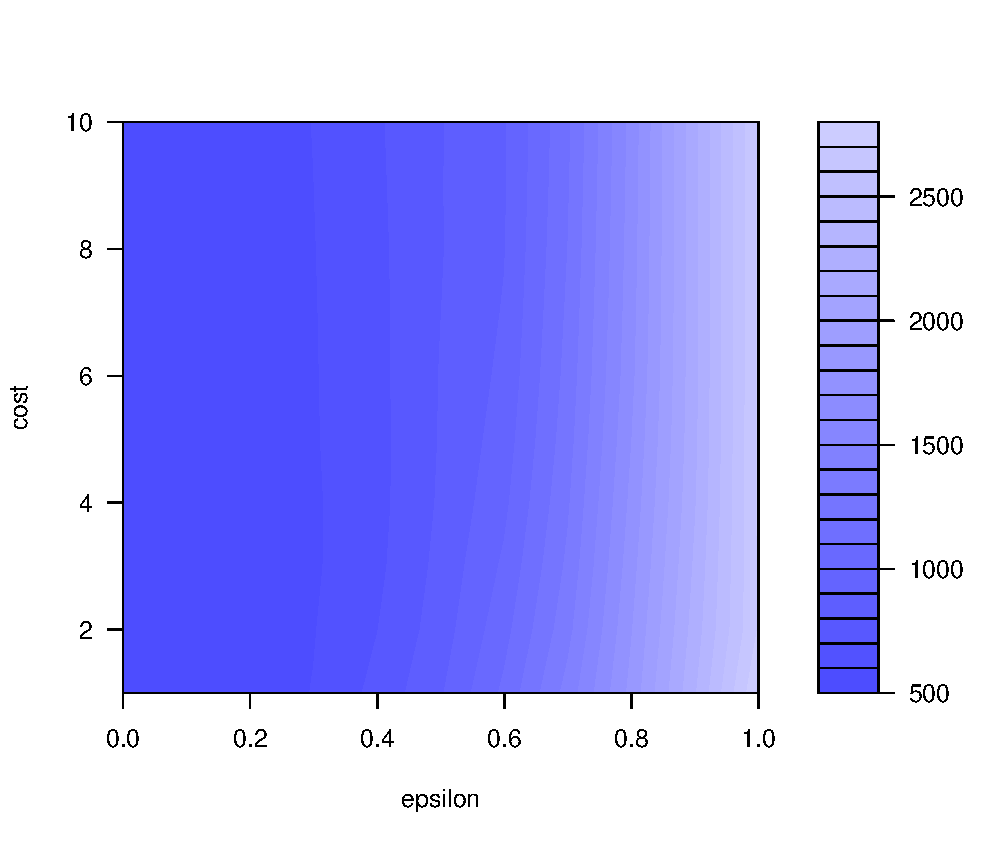
\includegraphics[width=0.65\textwidth]{./img/modeling/svm-dc}
			}
		}
		\end{adjustwidth}
		\caption{Tuning \ac{SVM} using $cost$ and $epsilon$ as the tuning parameters for head count (\ref{fig:tuning-svm-hc}) and device count (\ref{fig:tuning-svm-dc}) in R with \texttt{e1071} library. The performance is measured using \ac{MSE}. More optimal model is indicated by darker color, i.e., lower \ac{MSE}.}
		\label{fig:tuning-svm}
	\end{figure}

	We present the result of \ac{SVM} regression tuning in~\autoref{fig:tuning-svm}. We measure the performance of the \ac{SVM} using mean squared error (\ac{MSE}), in which best result has lower \ac{MSE}. The best performance for head count prediction is at 171.1065 with $\epsilon=0$ and $cost=3$, while for device count prediction is at 514.226 with $\epsilon=0$ and $cost=1$. We can also see a trend of increasing \ac{MSE} as the $epsilon$ increases.
	% hc============
	% Parameter tuning of 'svm':

	% - sampling method: 10-folds cross validation 

	% - best parameters:
	%  epsilon cost
	%        0    3

	% - best performance: 171.1065 


	% dc============
	% Parameter tuning of 'svm':

	% - sampling method: 10-folds cross validation 

	% - best parameters:
	%  epsilon cost
	%        0    1

	% - best performance: 514.226 

To summarize the regression analysis and to interpret the result, we use another approach to calculate the error, which has more intuitive interpretation. We use residual error, which can be formulated as
\begin{equation}\label{eq:residual-error}
	\bar { error } =\frac { 1 }{ n } \left( \sum _{ i=1 }^{ n }{ \left| { p }_{ i }-{ a }_{ i } \right|  }  \right) 
\end{equation}
where ${ p }_{ i }$ is the predicted value and ${ a }_{ i }$ is the actual value. As formulated in the equation, residual error shows mean of the difference between predicted and actual value. Using the optimum model of each regression technique, we perform another 10-fold cross validation to obtain residual error measurement. The optimal model has a residual error closer to zero.

\begin{table}[h]
\centering
\caption{Summary of regression analysis showing the range of the data and the residual error of each regression method.}
\label{tab:regression-summary}
\begin{tabular}{llllll}
\toprule
                   & \multicolumn{2}{c}{Value Range}                         & \multicolumn{3}{c}{Residual Error}                                                        \\
                   & \multicolumn{1}{c}{Min} & \multicolumn{1}{c}{Max} & \multicolumn{1}{c}{Linear} & \multicolumn{1}{c}{k-NN} & \multicolumn{1}{c}{SVM} \\ \midrule
Head count estimation   & 0                       & 115                     & 9.89                                  & 7.05                    & 7.06                    \\
Device count estimation & 0                       & 288                     & 23.81                                 & 13.14                   & 13.34                  \\ \bottomrule
\end{tabular}
\end{table}

\autoref{tab:regression-summary}~presents the summary of the regression analysis. Non-linear regression has better performance than the linear regression. \ac{k-NN} and \ac{SVM} do not have much difference of error for both head count and device count estimation. Device count estimation has wider value range and error compared to head count estimation.

% Plot the prediction graph in each cross validation round, then combined.
% Explain the result in percentage as well, instead of manual count. -> for the error in the modeling.
% plot the graph of head count (real vs predicted) vs parameters (ap count, or anything else)
% present the evaluation in people count and also percentage









\section{Discussion} % (fold)
\label{sec:discussion}
We discuss our findings of the experiments in the following topics, ambient noise recording, ground truth approximation, scanning time effect, sensor readings correlations, and the limitation of the present study.

	\subsection{Ambient Noise Recording} % (fold)
	\label{sub:ambient_noise_recording}
	We recorded ambient noise and extracted the peak-level (\ac{PKLV}) and root-mean-square (\ac{RMS}) of the recordings, which are highly correlated each other, with $\rho=0.77$ (see~\autoref{fig:scatterplot-matrix}). Initially, we expect to see a strong correlation of ambient noise and the level of social density, i.e., the location which has high level of social density also has high value of ambient noise, but the result says otherwise. We can see in scatter plot matrix of the dataset, \autoref{fig:scatterplot-matrix}, that only the correlation of head count and peak level which is more than $0.5$ ($\rho=0.58$). The other correlations of social density level (head count or device count) and ambient noise (peak level or root-mean-square) are below $0.5$.

	In the scatter plot of~\autoref{fig:scatterplot-matrix}, we can see that some of the low social density values (less than 20) have high ambient noise value as well (more than -20dB), which means we also observed more noise in the area where less crowd was observable. However, we can also see in~\autoref{fig:scatterplot-matrix} that no high social density values (more than 50 for device count and 20 for head count) are below -30dB, which means high social density areas have high amount of noise. We can conclude that high values of ambient noise mostly indicate a high level of social density. The line charts showing the peak level and root-mean-square of the ambient noise of all locations (\autoref{fig:audio-result-day1}, \autoref{fig:audio-result-day2}, \autoref{fig:audio-result-day3}, and \autoref{fig:audio-result-day4}) also support our conclusion. The graphs show that more crowded locations (Grote Markt and Paddepoel) have higher peak level or root-mean-square value than (Home and remote area) less crowded locations although some overlaps exist.

	Furthremore, microphone sensitivity also affects the result of ambient noise recording. We used laptop's built-in microphone to record the ambient noise. These microphones (and ones installed in smartphones) are attuned to a specific (and rather narrow) range of sound intensity.

	% https://support.biamp.com/General/Audio/Microphone_sensitivity
	% http://electronics.stackexchange.com/questions/59157/over-what-frequency-range-can-the-microphone-of-smartphone-receive-the-sound
	% http://www.makeuseof.com/tag/great-tips-recording-audio-smartphone-tablet/
	% http://www.scienceprog.com/long-range-directional-microphones-myth-and-reality/
	% http://www.epanorama.net/newepa/2014/09/08/sound-level-measuring-with-android-phone/
	% seems legit http://www.analog.com/library/analogdialogue/archives/46-05/understanding_microphone_sensitivity.html?doc=an-1328.pdf


	\subsection{Ground Truth Approximation} % (fold)
	\label{sub:ground_truth_approximation}
	We estimate the crowd count as a first approximation of the ground truth because it is known that getting the ground truth of crowd density in public spaces is difficult~\cite{thesis041}. We used time-lapse image based, which works by manually counting heads in the images, and WiFi's probe request based technique, works by counting unique \ac{MAC} addresses.
	% Both methods rely on predefined assumptions, which say .

	Although probe request based estimation is promising, some drawbacks are also present. In this method, we are not able to distinguish the type of devices, i.e., whether it is a smartphone, tablets, or computers. Although one mostly brings a smartphone~\cite{thesis047}, which means we can deduce that a smartphone means a person present, there is also a possibility that one brings more devices or no devices at all.

	Furthermore, WiFi based technique is able to detect object through walls, which could be good or bad depending on the perspective. In indoor social density estimation, this is a bad approximation because WiFi might detect some people but in fact there are way less or no people at all inside a room, as they are located in another room nearby. This is a potential threat, for instance, if our method detects some people but actually no one is present in the room. However, in outdoor social density estimation, WiFi based technique performs better than image based technique, as WiFi can see people through an obstacle, while image-based cannot. To sum up, we have to be more careful in doing indoor monitoring. As an option, we can also combine the social density estimation with ambient recording to see whether there is a noise inside a room, as empty room is mostly quite. 
	
	Compared to the probe request based estimation, time-lapse image based technique cannot detect people through walls or buildings. This may be the reason why the image based technique detects less people than the WiFi based technique (see~\autoref{fig:total-population}). Furthermore, image based technique relies heavily on assumptions when vehicles, e.g., buses or cars, are captured in the image, as vehicles have very limited visual appearance of the people inside. We assume that there are a person in a car and five people in a bus. This assumptions may slightly bias the result.

	\subsection{Scanning Time Effect} % (fold)
	\label{sub:scanning_time_effect}
	We tested the effect of scanning time to investigate whether scanning time can potentially affect the outcomes. An interesting findings about the scanning time are shown in~\autoref{fig:time-effect}. We can see that the device count in each scanning time has different outcome, while the \ac{AP} count remains stable no matter when the scanning was performed. When we scanned the surroundings in the morning (09:00h), the device count was less than the \ac{AP} count, as there were not so many people present. However, the trend changed when we performed the scanning at 12:00h, as the device count surpassed the \ac{AP} count. We can also see an increasing trend at scanning time performed at 15:00h and decreasing trend at 18:00h.
	If the trend continues, there might be lower device count than \ac{AP} count at night.

	The findings presented in~\autoref{fig:time-effect} indicates that we also have to note the scanning time of the surroundings when the present study is implemented because different scanning time might have a very different outcome.

	\subsection{Correlation Between Sensor Readings and Social Density} % (fold)
	\label{sub:correlation_between_sensor_readings_and_social_density}
	The parameter which has a strong correlation with head count or device count is the \ac{AP} count, as shown in the top right of~\autoref{fig:scatterplot-matrix}. The correlation coefficients of \ac{AP} count vs device count, \ac{AP} count vs head count, and device count vs head count are 0.87, 0.85, and 0.86, respectively. We present in detail the correlation of head count, device count, and \ac{AP} count in~\autoref{sub:ap_and_social_density_correlation}.

	As we can see in the scatter plots of the correlation of \ac{AP}, \ac{DC}, and \ac{HC}, presented in~\autoref{fig:ap-dc-scatterplot}, \autoref{fig:ap-hc-scatterplot}, and \autoref{fig:hc-dc-scatterplot}, the lower social density data, as at home or remote area, seems to be more concentrated than higher social density data, as at Paddepoel or Grote Markt, and the higher social density data is widely spread. However, this does not mean that the frequency of high social density values is bigger than the low social density value. In fact, we have more data for lower social density than higher social density, as shown in the histograms of \ac{AP}, \ac{DC}, and \ac{HC} in~\autoref{fig:scatterplot-matrix}.

	If we look at~\autoref{fig:ap-dc-scatterplot}, \autoref{fig:ap-hc-scatterplot}, and \autoref{fig:hc-dc-scatterplot}, the data may also be used to perform a sort of localization, as each location shows different pattern. We can say that the \ac{AP} count is bound to an area, where each area has different social density level. Thus, this method is somewhat telling where the smartphone actually is and what the average of social density level in that area is. In the other way, we could possibly infer where the location of the smartphone is using our proposed technique, although further study may be required to support this opinion.

	% present the result of each location. and compare within days
	In the beginning, we expect that the number of \ac{AP} follows the fluctuation of the number of people in a certain location, as people might bring their own portable WiFi transmitter to assemble an ad-hoc \ac{AP}, which will add up the number of \ac{AP} available in the location. However, this turned out to be a rare situation, as we do not see any trend between number of people and \ac{AP} count, as shown in line chart of the experiment presented in~\autoref{ch:appendix-sensor-readings}.

	Moreover, if we see at the line chart, there is a fluctuation of \ac{AP} count, although actually available \ac{AP} count should be the same or stable across the time. This fluctuation might be caused by the instability of radio transmission that may affect the signal strength of the WiFi \ac{AP} and thus making some \ac{AP}s some not detected.
	
	Another interesting finding is that, it turned out that several \ac{AP}s are using the same \ac{SSID}, e.g., eduroam. This makes user only see one \ac{AP} available, in fact, those \ac{AP} are using different \ac{MAC} address.

	\subsection{Limitation of the Present Study}
	\label{sub:limitation_of_the_present_study}
	The proposed method has some limitations that limit its implementation.
	% #1: location: range, indoor outdoor
	The first limitation is the location. The proposed method only works at places where WiFi \ac{AP} use is not restricted, i.e., people are free to set up their own WiFi AP. Some locations where the use of WiFi is restricted exist, for instance, University of Groningen complex, where eduroam is the only the available AP and the occupants are discouraged to install their own AP. If we collect data from this location, we will possibly get uncorrelated \ac{AP} count and social density.

	Furthermore, our dataset consists of data collected from four different location. This dataset represents the situation of selected locations but possibly not for other locations, as other locations may have different characteristics. For instance, in developing countries or other locations where the use of WiFi are not common, the number of \ac{AP} in a public area may be much lower than what we have in our dataset.

	As we mainly work with WiFi, the range of the proposed social density follows the maximum WiFi coverage of the smartphone, which extends roughly from 20 to 50 meters. This range may be good or bad depending on the context. For outdoor situation, this range gives a good approximation as it is considerably broad enough to count social density. However, this range may be too broad for indoor implementation. For instance, we may get a result that says there are 20 people in total, but in fact there is only five or even less people in the room. This is because WiFi also detects people outside the room. However, we can also combine the result with ambient noise recording, as empty room are usually more quite.

	% Use wigle to explain that this could not be generalized. Mention comparison of one place and another place. in other cities or contries.

	% #2: time
	The other limitation is the time. Our dataset consists of data collected in daytime, ranging from 08:15h to 14:45h. Using this dataset, we are only able to approximate the level of social density if the new data is captured during the same time frame. If the new data is taken outside the time frame, our dataset is unable to tell the level of social density. This fact is based on the time of scanning investigation described in~\autoref{ssub:effect_of_scanning_time} and \autoref{sub:effect_of_scanning_time}.
	

	

% conclusion
In conclusion, the results indicate that locations with high level of social density tend to have more access points. WiFi \ac{AP} shows the strongest correlation with the social density level, followed by \ac{RMS} that reveals a weaker correlation with social density level. Thus, we can say that it is possible to infer social density level from smartphone sensor readings. To achieve better accuracy, we may implement classification analysis instead of regression. However, regression analysis yields class-based result instead of continuous numerical result.

Furthermore, generalization of this method requires further investigation in more locations and time, as other location may reveal different patterns.
% Although the data say that there are minor variation in days, other locations may have higher variation.
Scanning time result also says that scanning time affects the social density level. Moreover, the settings may vary in cities or even countries.

% We can also see the result explain about this method could works as a localization method, could be useful especially if GPS signal is not available
% also use % https://wigle.net/ database of public WiFi
% We also select daytime as the preferred scanning time because that is the time when most crowd are observable. This implies that our collected data resemble only daytime duration, meaning that conclusion might only be able to deduct for daytime.

% Question: Does weather affect WiFi performance?

%*****************************************
%*****************************************
%*****************************************
%*****************************************
%*****************************************
% mac address randomization
% mention about the randomization as well, that that might not a solution, mention the paper that comprehensively discuss about the randomization
% explain that the IE (information elements on probe request) method is not really 100\% correct.
% prove it by using LG nexus randomized and real probe request.
% To avoid randomized mac, we use discretized monitoring, instead of doing it continuously for a long time, we did it in separate scanning interval.
% Why dont you use 2 devices for separate purpose? one for probe request and one for access point.
% When android is in energy saving mode, the OS prohibits any app for doing WiFi Scan or any other scan.
% why the some SN disappear.
%!TEX root = ../thesis-guntur.tex
%************************************************
\chapter{Conclusion and Future Work}
\label{ch:conclusion-future-work} % $\mathbb{ZNR}$
%************************************************
We have studied how a consumer smartphone can be utilized as an instrument to estimate the level of social density in the surroundings of its owner. We collected the data at several locations to see the trend of sensor readings and social density level. We also try to construct a model to predict upcoming social density levels based on sensor readings. To conclude this thesis, we go through the research questions and answer the question based on our findings. As posed in~\autoref{ch:introduction}, the main research question is

\begin{displayquote}\textit{
How can we estimate the level of social density of the surroundings using smartphone as a passive behavioral monitoring scheme?}
\end{displayquote}

\noindent
As presented in~\autoref{ch:literature-review}, literature study shows that smartphone sensors are exploitable to estimate the social density level of the surroundings. We also conducted experiments, described in~\autoref{ch:experimental-setup} to inspect the hypothesis. The results, presented in~\autoref{ch:results}, show that there is a trend that follows the relation of sensor readings and social density levels. We also discuss the findings and develop a regression model to predict the social density level in~\autoref{ch:regression-and-discussion}.

The sub-questions are defined to help answering and validating the main research question. Those were formulated as follows:
\begin{enumerate}
	\item \textit{What sensors are available at consumer smartphone and which of those are favorable for the social density estimation method?}\\
	We present a summary of available sensors in smartphone in~\autoref{tab:smartphone-sensor-summary}. In this thesis, we make use of WiFi and microphone to record data for estimating social density level. We select these sensors as those are usable no mater how the smartphone is operated and positioned.

	\item \textit{How can we validate the sensor readings, meaning, to get the ground truth or the approximation of the ground truth?}\\
	We use manual head counting in time-lapse images and unique \ac{MAC} address counting in captured WiFi probe request packets as first approximation of ground truth. We select these techniques as those are demonstrated to have a correlation with social density in the surroundings.

	% \item \textit{How to overcome or minimize the challenges of this technique?}\\

	\item \textit{Can this method work everywhere? What is the scope of this method?}\\
	Our proposed method works well at the selected locations of the experiment presented in~\autoref{tab:location-summary}. Our method is applicable in locations where WiFi \ac{AP} use is not restricted, i.e., people are free to set up their own WiFi \ac{AP} in anyway they prefer. Furthermore, our method is bound to time constraint, which limits to daytime implementation when the social density level reaches its peak. Generalization of this method requires further data collection.
\end{enumerate}

\section{Future Work} % (fold)
\label{sec:future_work}
We plan to collect more data so that we can generalize the proposed method. The data collection includes more locations with several scanning time to see the variance of social density in time, adding more features for analysis. Furthermore, we are also interested in doing classification analysis to see whether we can achieve better performance of social density estimation. However, classification analysis means that the result will be classified into several classes instead of continuous numbers.

\added{
Moreover, we plan to enrich the smartphone data by the inclusion of other data types, for instance, \ac{GPS} location and nearby Bluetooth signals. Different data type inclusion may result in better model of social density information, so that we can achieve more accurate results. Other resources or instruments may refer to using dedicated device to monitor the social density level or other data coming from third party stakeholders such as cellular operators.
}

% explain about this method could works as a localization method, could be useful especially if GPS signal is not available
%*****************************************
%*****************************************
%*****************************************
%*****************************************
%*****************************************

%\include{multiToC} % <--- just debug stuff, ignore for your documents
% ********************************************************************
% Backmatter
%*******************************************************
\appendix
%\renewcommand{\thechapter}{\alph{chapter}}
% \cleardoublepage
% \part{Appendix}

%!TEX root = ../thesis-guntur.tex
%********************************************************************
% Appendix
%*******************************************************
% If problems with the headers: get headings in appendix etc. right
%\markboth{\spacedlowsmallcaps{Appendix}}{\spacedlowsmallcaps{Appendix}}
\chapter{Access Point Count Correlation}
\label{ch:appendix-sensor-readings}

\section{Scatter Plots} % (fold)
\label{sec:scatter-plots}
% ap vs head count
\begin{figure}[H]
  \begin{adjustwidth}{-1cm}{}
  \centering
  \subfloat[day 1]{
    \label{fig:ap-hc-day1}{
      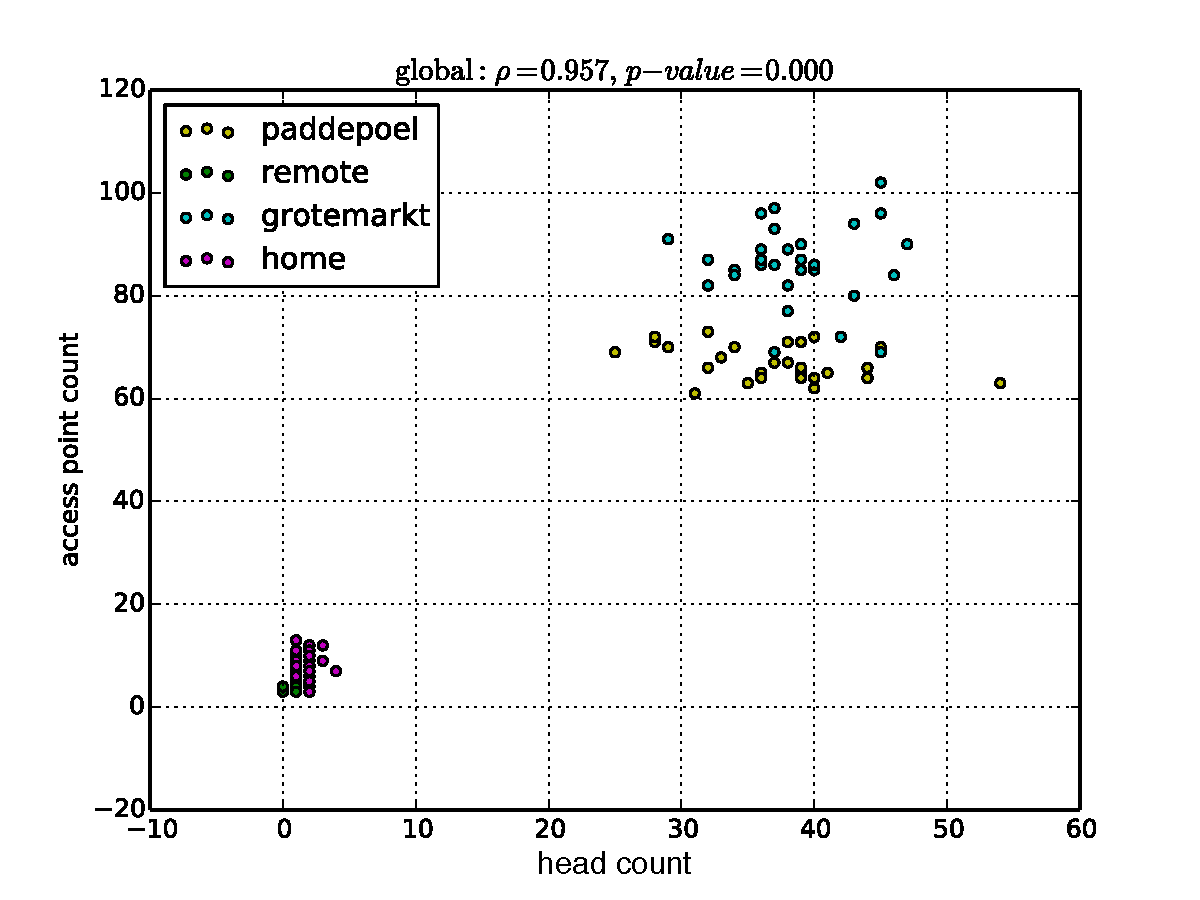
\includegraphics[width=0.7\textwidth]{./img/result/day/day1/global-gt-vs-ap}
    }
  }
  \subfloat[day 2]{
    \label{fig:ap-hc-day2}{
      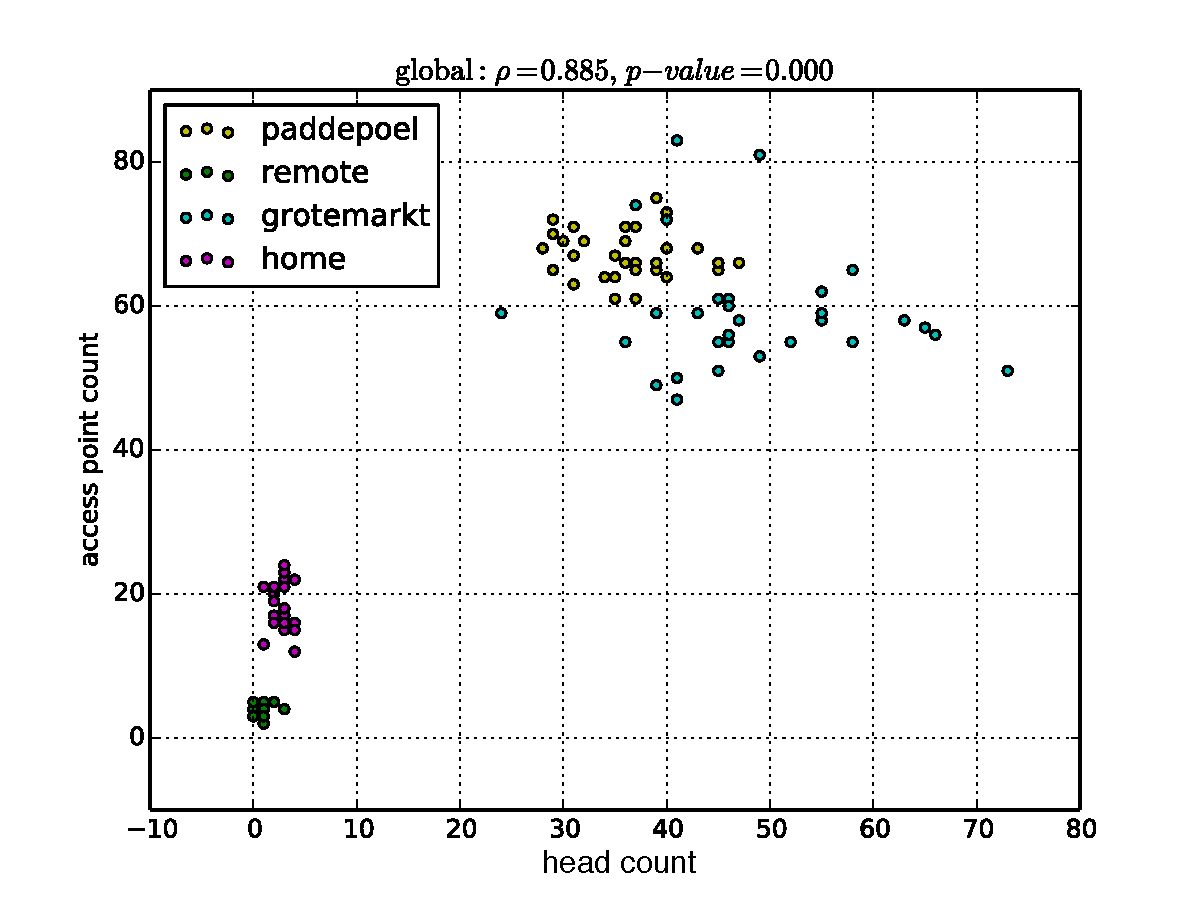
\includegraphics[width=0.7\textwidth]{./img/result/day/day2/global-gt-vs-ap}
    }
  }\\
  \subfloat[day 3]{
    \label{fig:ap-hc-day3}{
      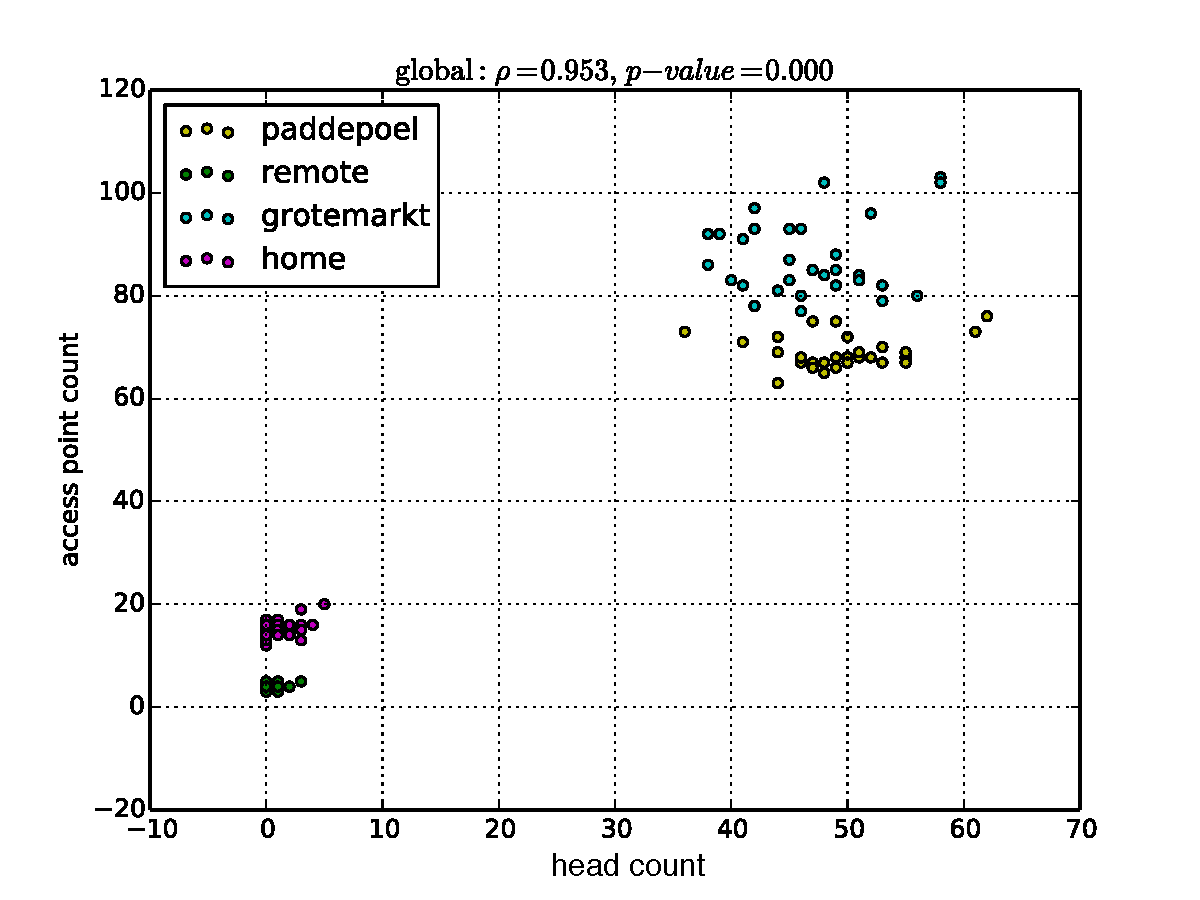
\includegraphics[width=0.7\textwidth]{./img/result/day/day3/global-gt-vs-ap}
    }
  }
  \subfloat[day 4]{
    \label{fig:ap-hc-day4}{
      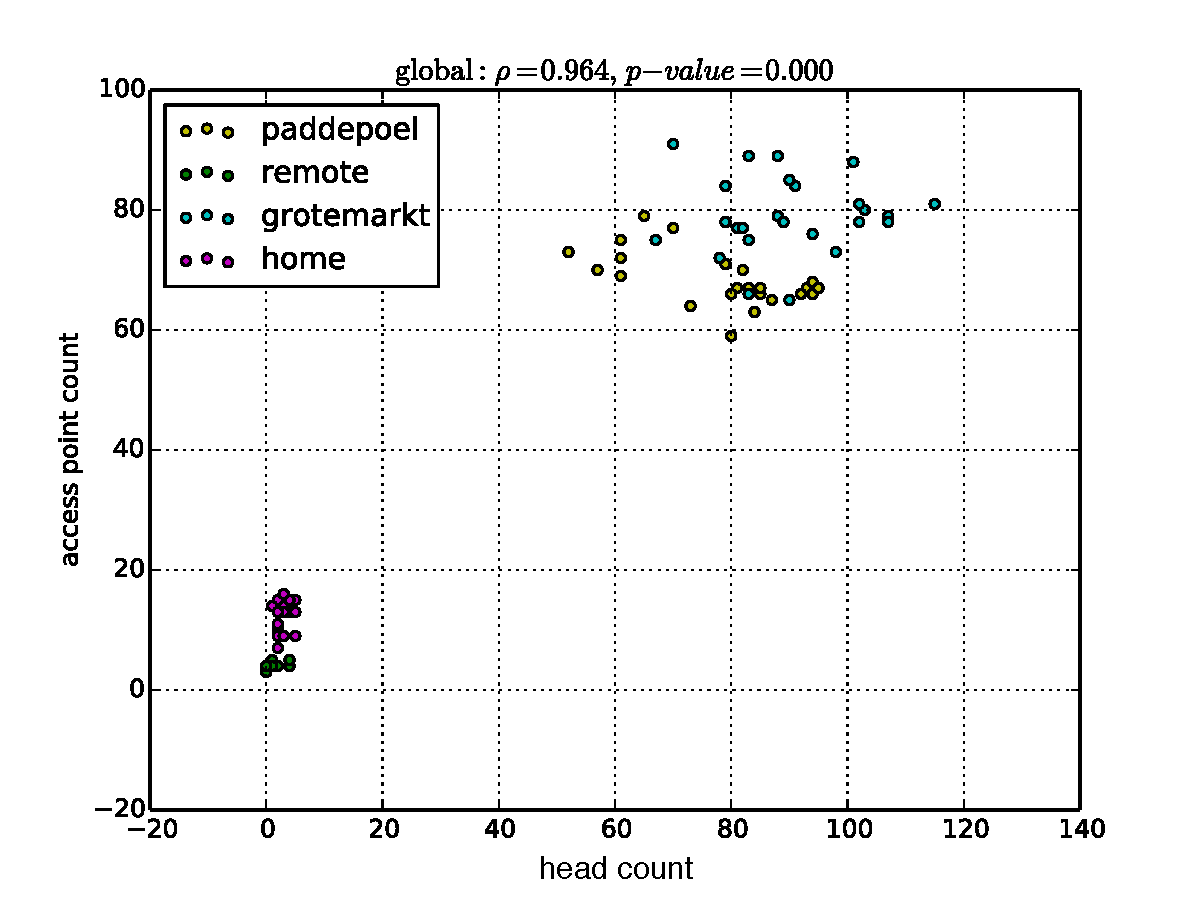
\includegraphics[width=0.7\textwidth]{./img/result/day/day4/global-gt-vs-ap}
    }
  }
  \end{adjustwidth}
  \caption[The scatter plots of the correlation between headcount and \ac{AP} count.]
  {The scatter plots showing the correlation between headcount and \ac{AP} count in four days of experiment. The location is coded in color.}
  \label{fig:ap-hc-scatterplot}
\end{figure}

% ap vs device count
\begin{figure}[H]
  \begin{adjustwidth}{-4cm}{}
  \centering
  \subfloat[day 1]{
    \label{fig:ap-dc-day1}{
      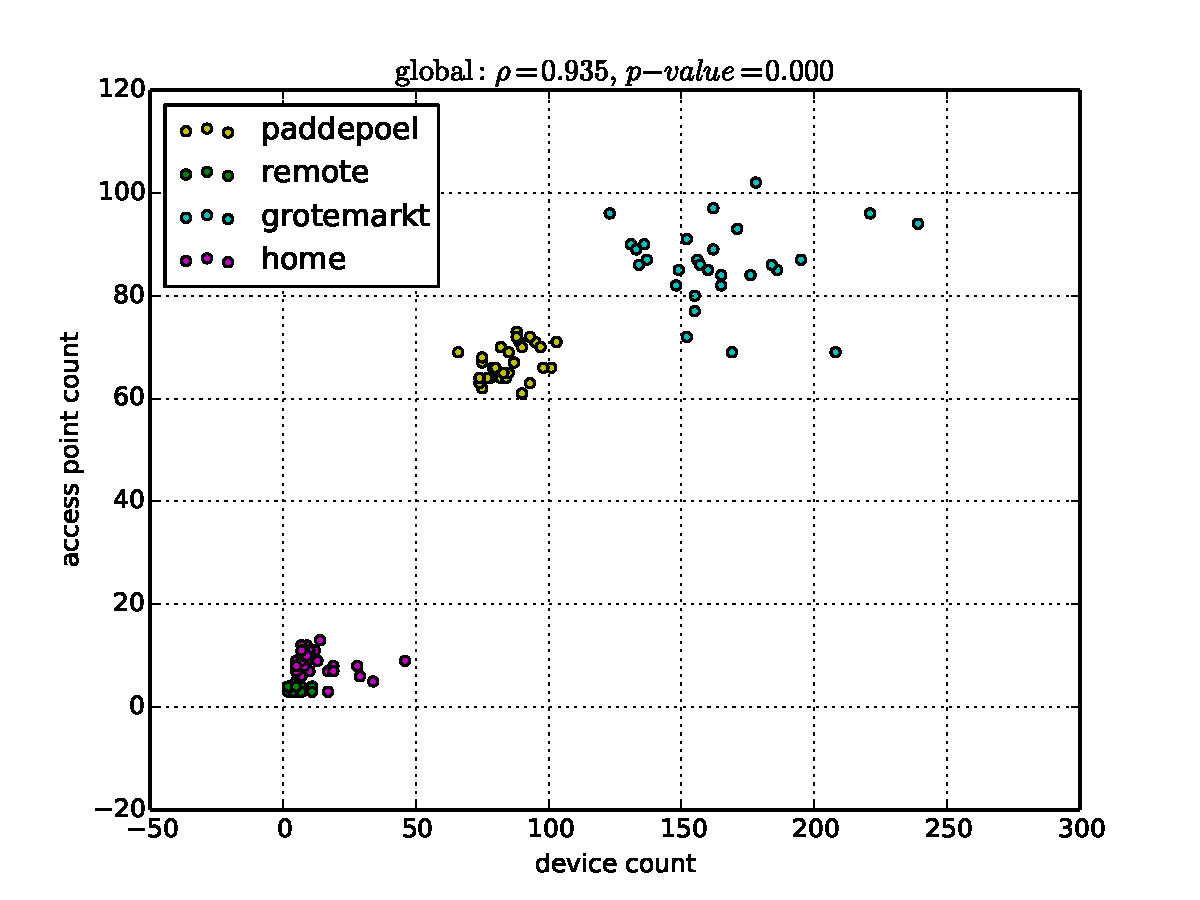
\includegraphics[width=0.7\textwidth]{./img/result/day/day1/global-pr-vs-ap}
    }
  }
  \subfloat[day 2]{
    \label{fig:ap-dc-day2}{
      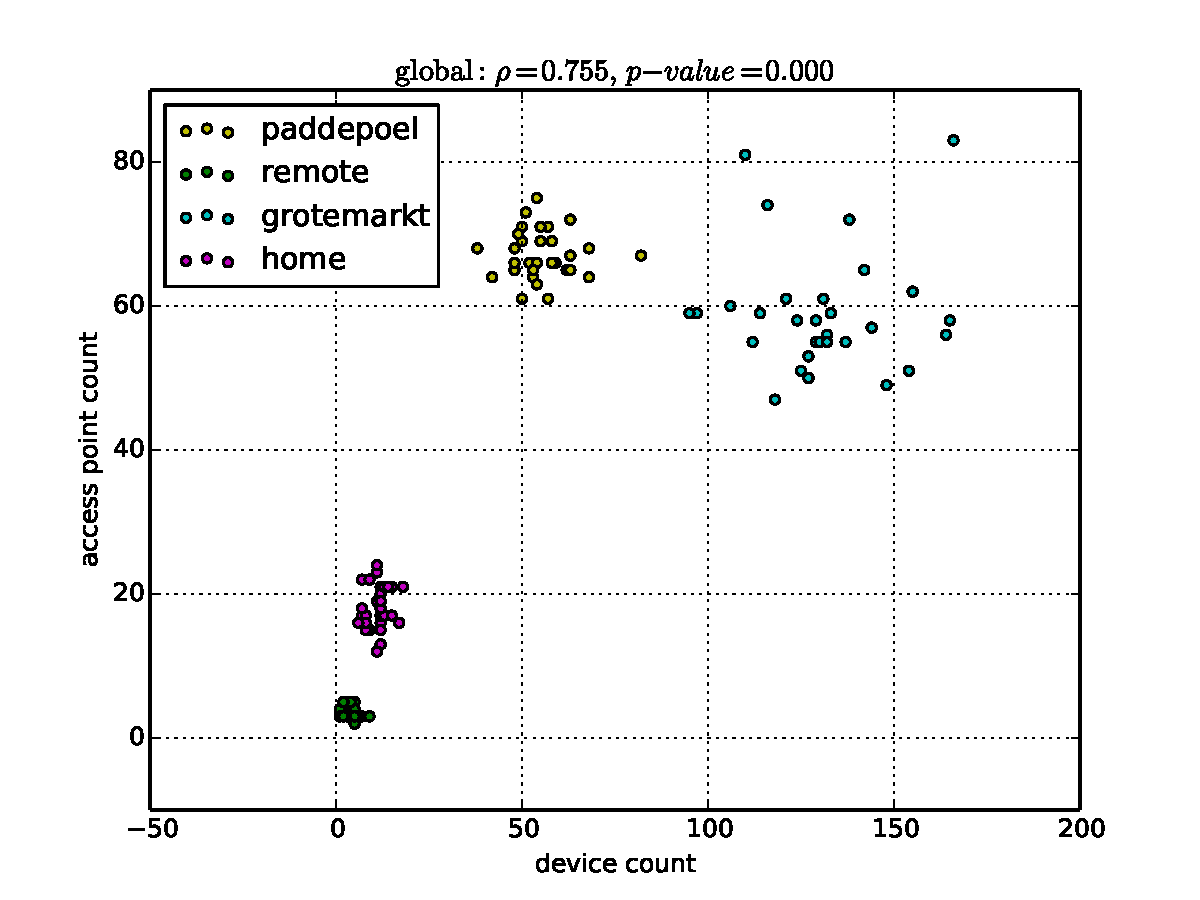
\includegraphics[width=0.7\textwidth]{./img/result/day/day2/global-pr-vs-ap}
    }
  }\\
  \subfloat[day 3]{
    \label{fig:ap-dc-day3}{
      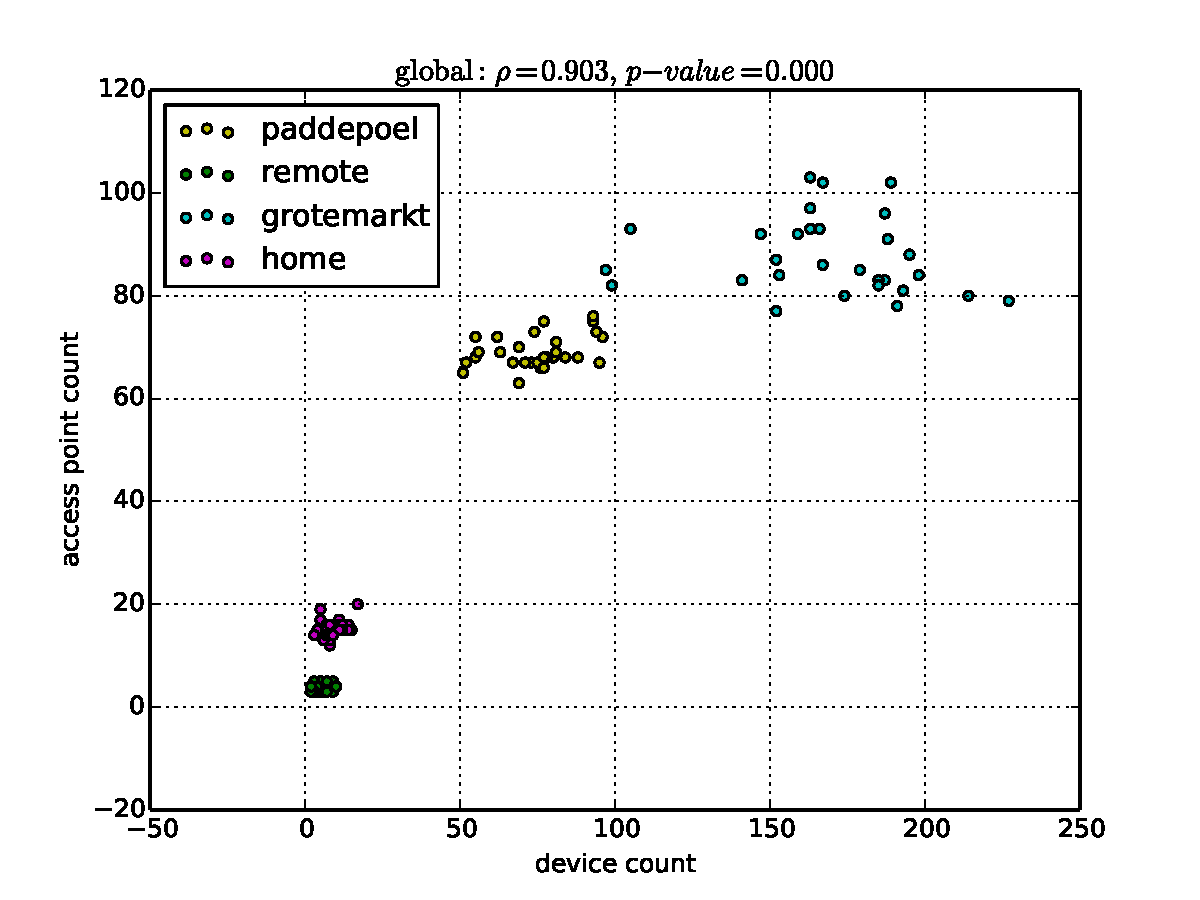
\includegraphics[width=0.7\textwidth]{./img/result/day/day3/global-pr-vs-ap}
    }
  }
  \subfloat[day 4]{
    \label{fig:ap-dc-day4}{
      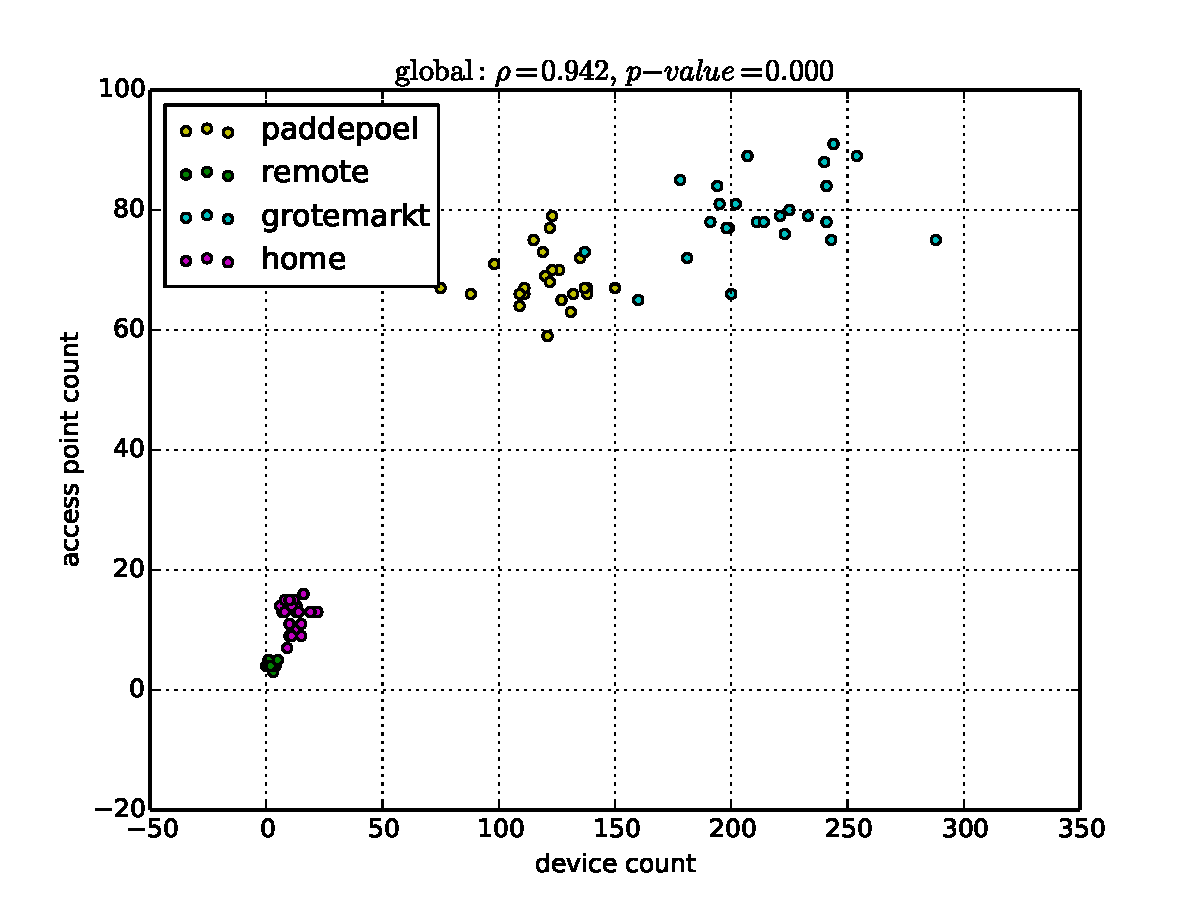
\includegraphics[width=0.7\textwidth]{./img/result/day/day4/global-pr-vs-ap}
    }
  }
  \end{adjustwidth}
  \caption[The scatter plots of the correlation between device count and \ac{AP}.]
  {The scatter plots showing the correlation between device count and \ac{AP} count in four days of experiment. The location is coded in color.}
  \label{fig:ap-dc-scatterplot}
\end{figure}

% ap vs device count
\begin{figure}[H]
  \begin{adjustwidth}{-1cm}{}
  \centering
  \subfloat[day 1]{
    \label{fig:hc-dc-day1}{
      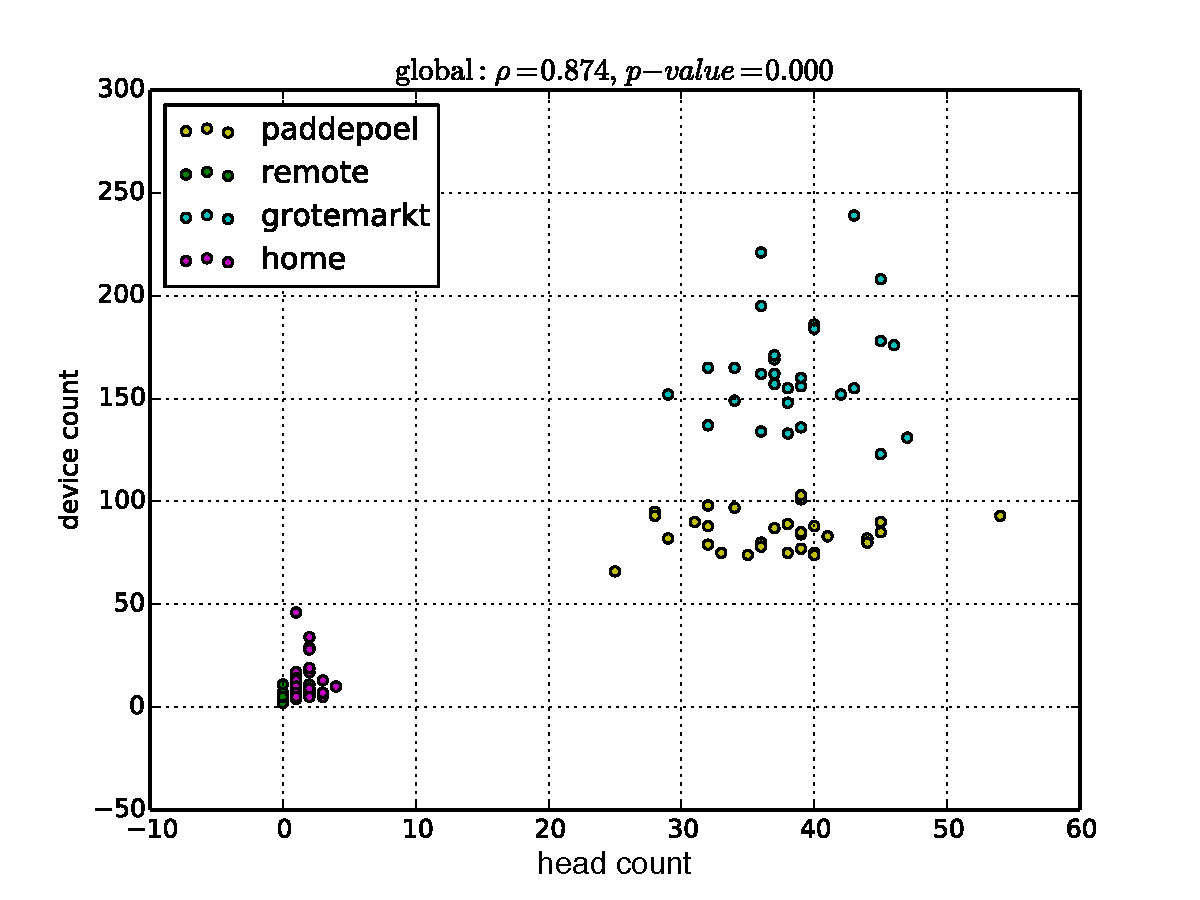
\includegraphics[width=0.7\textwidth]{./img/result/day/day1/global-gt-vs-pr}
    }
  }
  \subfloat[day 2]{
    \label{fig:hc-dc-day2}{
      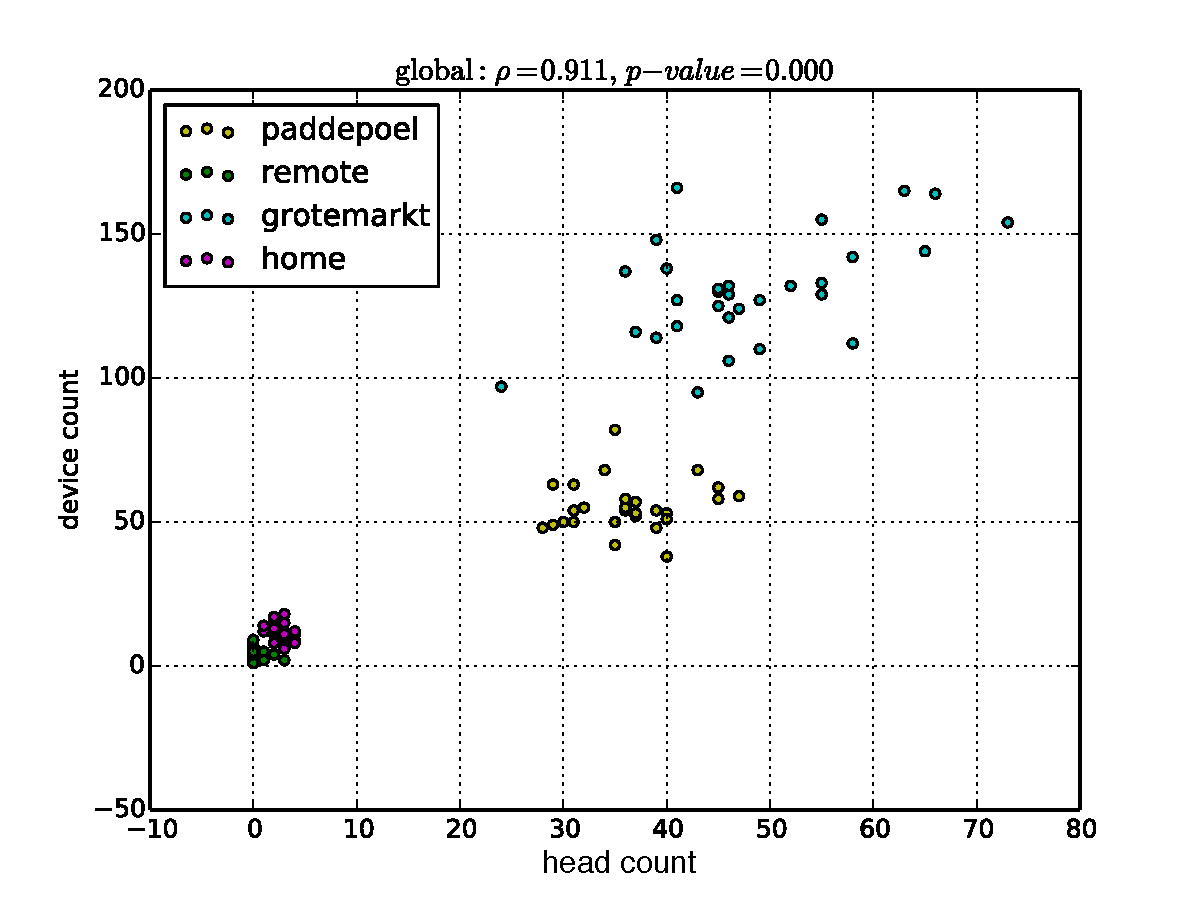
\includegraphics[width=0.7\textwidth]{./img/result/day/day2/global-gt-vs-pr}
    }
  }\\
  \subfloat[day 3]{
    \label{fig:hc-dc-day3}{
      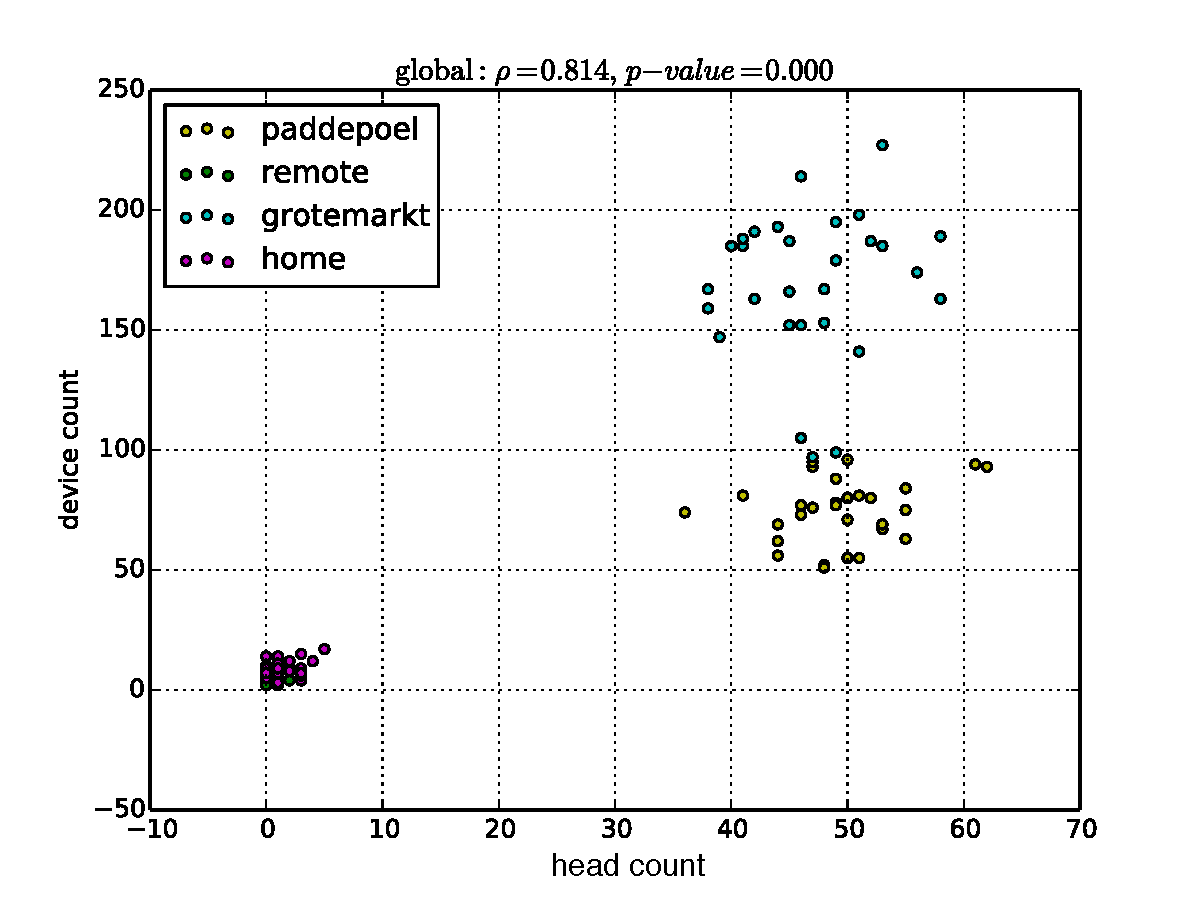
\includegraphics[width=0.7\textwidth]{./img/result/day/day3/global-gt-vs-pr}
    }
  }
  \subfloat[day 4]{
    \label{fig:hc-dc-day4}{
      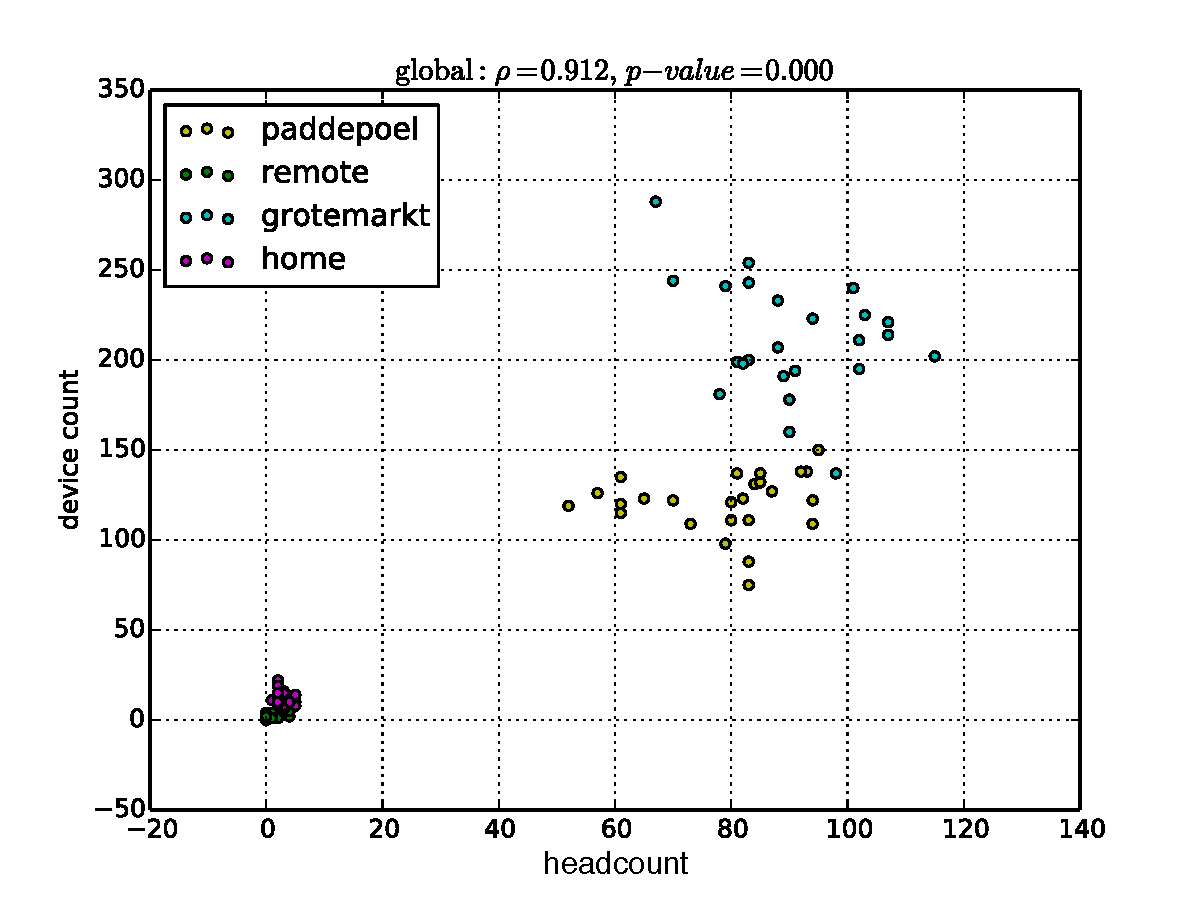
\includegraphics[width=0.7\textwidth]{./img/result/day/day4/global-gt-vs-pr}
    }
  }
  \end{adjustwidth}
  \caption[The scatter plots of the correlation between device count and \ac{AP} count.]
  {The scatter plots showing the correlation between device count and \ac{AP} count in four days of experiment. The location is coded in color.}
  \label{fig:hc-dc-scatterplot}
\end{figure}







\section{Line charts} % (fold)
\label{sec:line_charts}

\begin{figure}[H]
  \begin{adjustwidth}{-4.5cm}{}
  \centering
  \subfloat[day 1]{
    \label{fig:remote-day1}{
      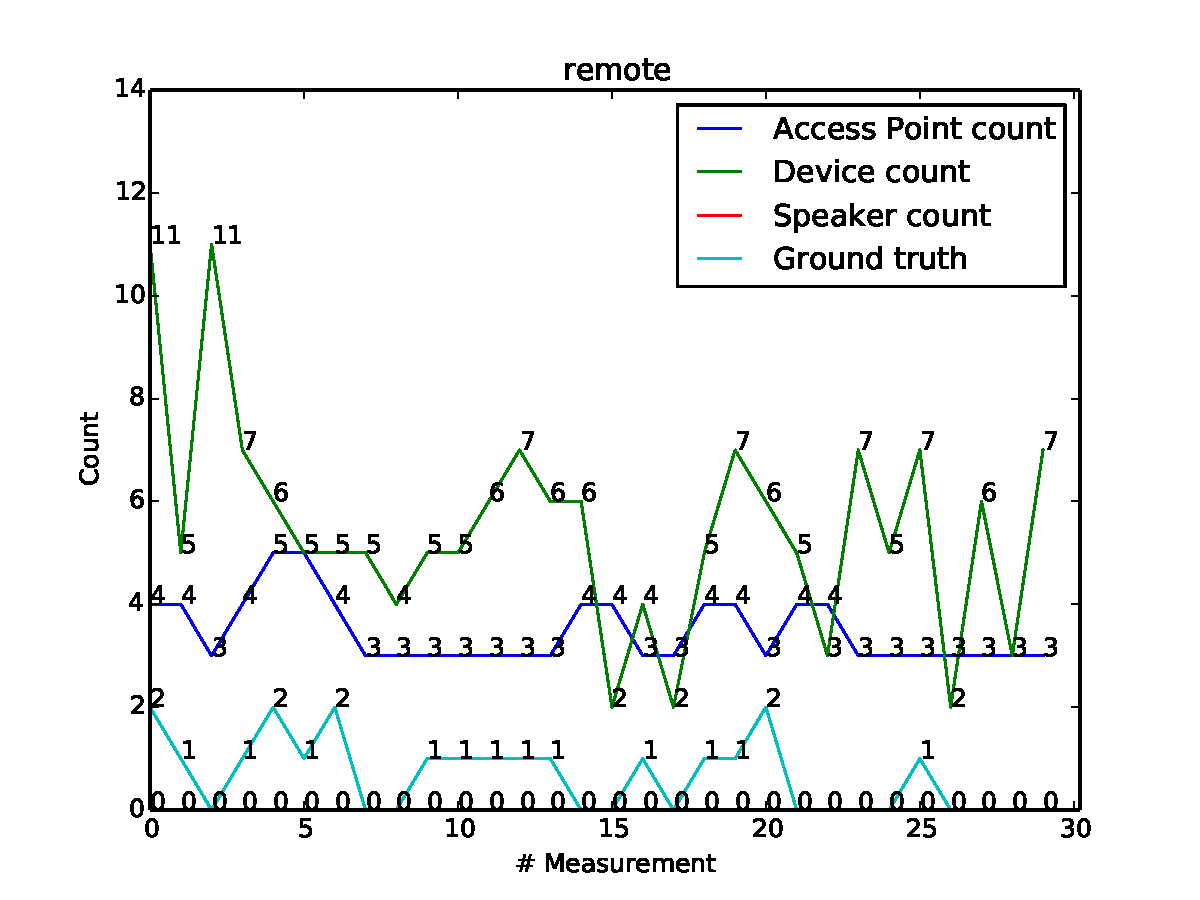
\includegraphics[width=0.7\textwidth]{./img/result/day/day1/remote-20161026}
    }
  }
  \subfloat[day 2]{
    \label{fig:remote-day2}{
      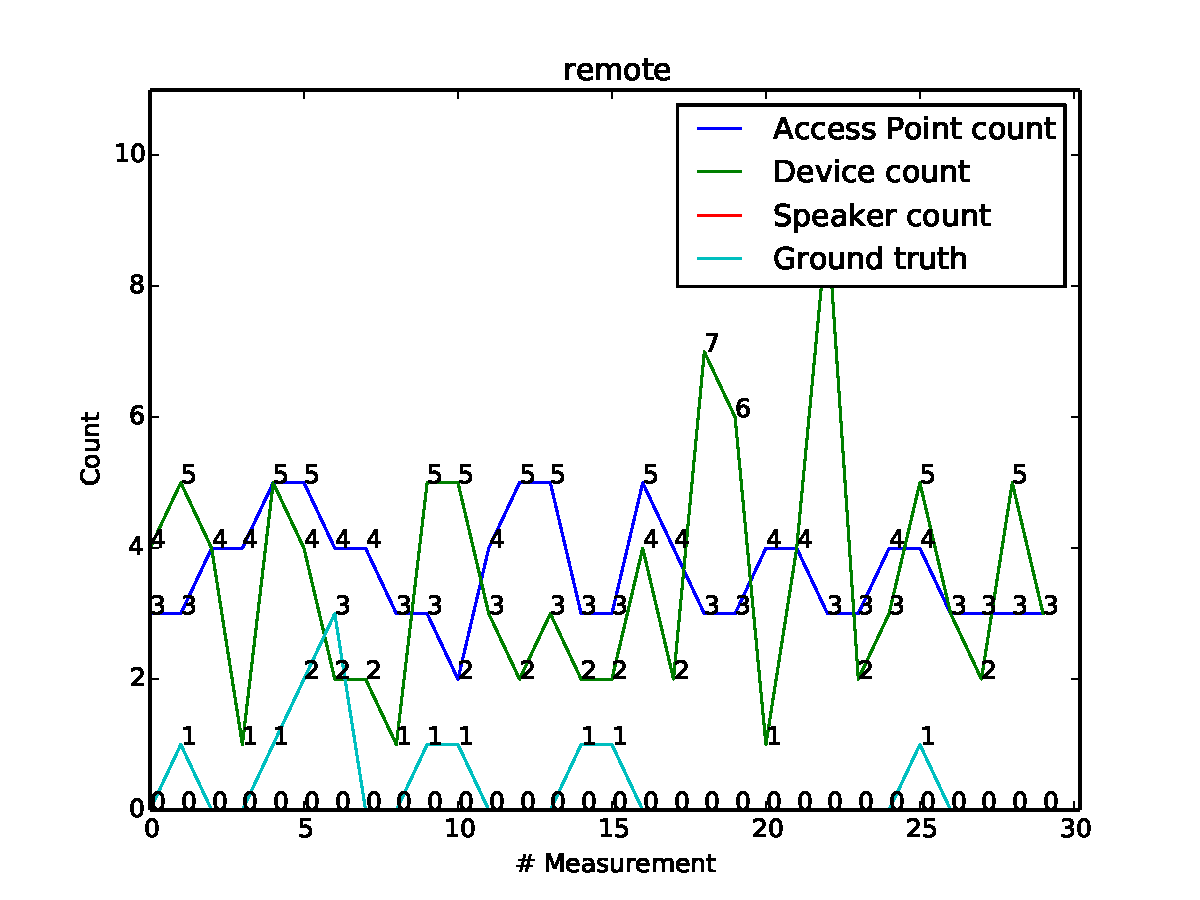
\includegraphics[width=0.7\textwidth]{./img/result/day/day2/remote-20161027}
    }
  }\\
  \subfloat[day 3]{
    \label{fig:remote-day3}{
      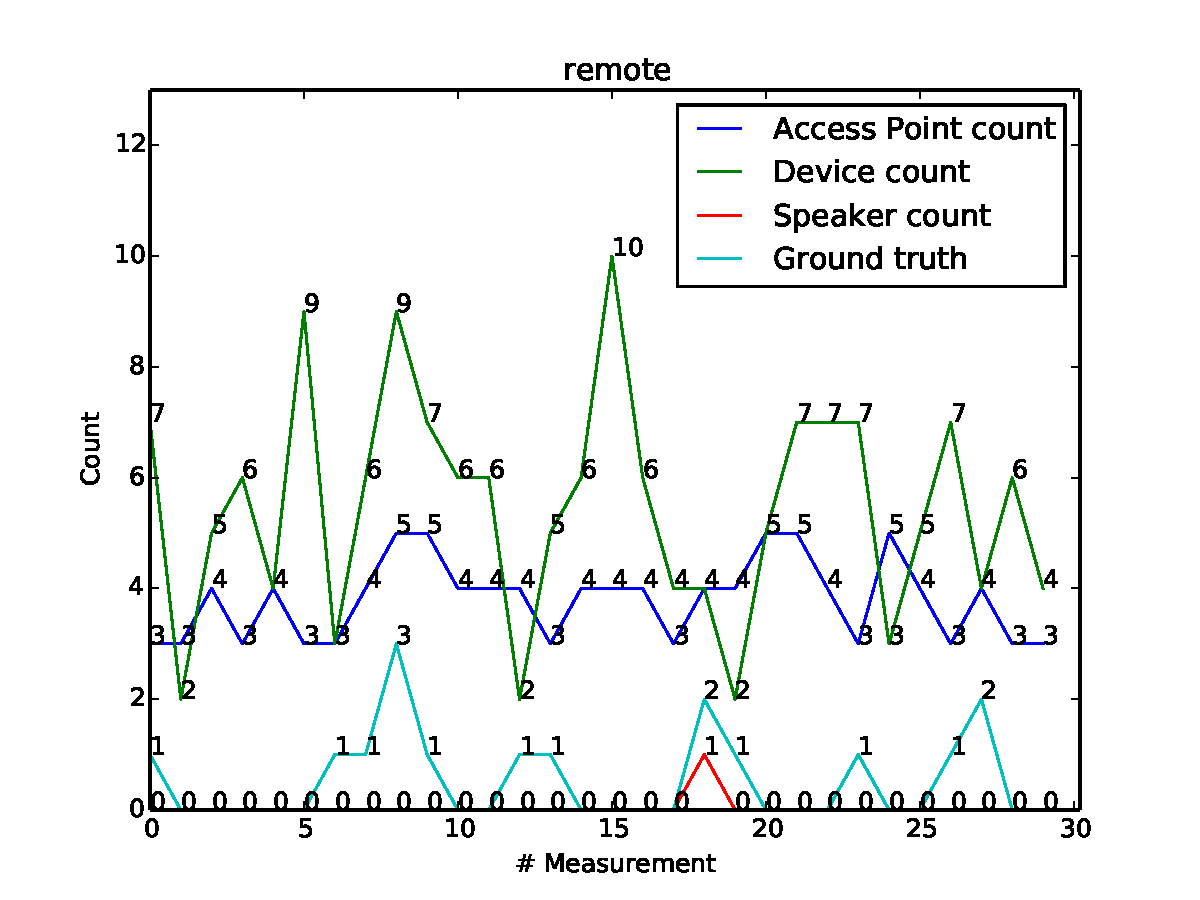
\includegraphics[width=0.7\textwidth]{./img/result/day/day3/remote-20161028}
    }
  }
  \subfloat[day 4]{
    \label{fig:remote-day4}{
      \includegraphics[width=0.7\textwidth]{./img/result/day/day4/remote-20161029}
    }
  }
  \end{adjustwidth}
  \caption[The line chart of sensor readings at remote area.]
  {The line chart of sensor readings at \textit{remote area} in four days of experiment.}
  \label{fig:result-remote-line-chart}
\end{figure}


\begin{figure}[H]
  \begin{adjustwidth}{-1cm}{}
  \centering
  \subfloat[day 1]{
    \label{fig:home-day1}{
      \includegraphics[width=0.7\textwidth]{./img/result/day/day1/home-20161026}
    }
  }
  \subfloat[day 2]{
    \label{fig:home-day2}{
      \includegraphics[width=0.7\textwidth]{./img/result/day/day2/home-20161027}
    }
  }\\
  \subfloat[day 3]{
    \label{fig:home-day3}{
      \includegraphics[width=0.7\textwidth]{./img/result/day/day3/home-20161028}
    }
  }
  \subfloat[day 4]{
    \label{fig:home-day4}{
      \includegraphics[width=0.7\textwidth]{./img/result/day/day4/home-20161029}
    }
  }
  \end{adjustwidth}
  \caption[The line chart of sensor readings at home.]
  {The line chart of sensor readings at \textit{home} in four days of experiment.}
  \label{fig:result-home-line-chart}
\end{figure}


\begin{figure}[H]
  \begin{adjustwidth}{-5cm}{}
  \centering
  \subfloat[day 1]{
    \label{fig:paddepoel-day1}{
      \includegraphics[width=0.7\textwidth]{./img/result/day/day1/paddepoel-20161026}
    }
  }
  \subfloat[day 2]{
    \label{fig:paddepoel-day2}{
      \includegraphics[width=0.7\textwidth]{./img/result/day/day2/paddepoel-20161027}
    }
  }\\
  \subfloat[day 3]{
    \label{fig:paddepoel-day3}{
      \includegraphics[width=0.7\textwidth]{./img/result/day/day3/paddepoel-20161028}
    }
  }
  \subfloat[day 4]{
    \label{fig:paddepoel-day4}{
      \includegraphics[width=0.7\textwidth]{./img/result/day/day4/paddepoel-20161029}
    }
  }
  \end{adjustwidth}
  \caption[The line chart of sensor readings at Paddepoel Shopping Center.]
  {The line chart of sensor readings at \textit{Paddepoel Shopping Center} in four days of experiment.}
  \label{fig:result-paddepoel-line-chart}
\end{figure}


\begin{figure}[H]
  \begin{adjustwidth}{-1cm}{}
  \centering
  \subfloat[day 1]{
    \label{fig:grotemarkt-day1}{
      \includegraphics[width=0.7\textwidth]{./img/result/day/day1/grotemarkt-20161026}
    }
  }
  \subfloat[day 2]{
    \label{fig:grotemarkt-day2}{
      \includegraphics[width=0.7\textwidth]{./img/result/day/day2/grotemarkt-20161027}
    }
  }\\
  \subfloat[day 3]{
    \label{fig:grotemarkt-day3}{
      \includegraphics[width=0.7\textwidth]{./img/result/day/day3/grotemarkt-20161028}
    }
  }
  \subfloat[day 4]{
    \label{fig:grotemarkt-day4}{
      \includegraphics[width=0.7\textwidth]{./img/result/day/day4/grotemarkt-20161029}
    }
  }
  \end{adjustwidth}
  \caption[The line chart of sensor readings at Grote Markt.]
  {The line chart of sensor readings at \textit{Grote Markt} in four days of experiment.}
  \label{fig:result-grotemarkt-line-chart}
\end{figure}


%********************************************************************
% Other Stuff in the Back
%*******************************************************
\cleardoublepage%********************************************************************
% Bibliography
%*******************************************************
% work-around to have small caps also here in the headline
\manualmark
\markboth{\spacedlowsmallcaps{\bibname}}{\spacedlowsmallcaps{\bibname}} % work-around to have small caps also
%\phantomsection 
\refstepcounter{dummy}
\addtocontents{toc}{\protect\vspace{\beforebibskip}} % to have the bib a bit from the rest in the toc
\addcontentsline{toc}{chapter}{\tocEntry{\bibname}}
\label{app:bibliography}
\printbibliography

% \cleardoublepage%*******************************************************
% Declaration
%*******************************************************
\refstepcounter{dummy}
\pdfbookmark[0]{Declaration}{declaration}
\chapter*{Declaration}
\thispagestyle{empty}
Put your declaration here.
\bigskip
 
\noindent\textit{\myLocation, \myTime}

\smallskip

\begin{flushright}
    \begin{tabular}{m{5cm}}
        \\ \hline
        \centering\myName \\
    \end{tabular}
\end{flushright}

% \cleardoublepage\pagestyle{empty}

\hfill

\vfill


\pdfbookmark[0]{Colophon}{colophon}
\section*{Colophon}
This document was typeset using the typographical look-and-feel \texttt{classicthesis} developed by Andr\'e Miede. 
The style was inspired by Robert Bringhurst's seminal book on typography ``\emph{The Elements of Typographic Style}''. 
\texttt{classicthesis} is available for both \LaTeX\ and \mLyX: 
\begin{center}
\url{https://bitbucket.org/amiede/classicthesis/}
\end{center}
Happy users of \texttt{classicthesis} usually send a real postcard to the author, a collection of postcards received so far is featured here: 
\begin{center}
\url{http://postcards.miede.de/}
\end{center}
 
\bigskip

\noindent\finalVersionString

%Hermann Zapf's \emph{Palatino} and \emph{Euler} type faces (Type~1 PostScript fonts \emph{URW
%Palladio L} and \emph{FPL}) are used. The ``typewriter'' text is typeset in \emph{Bera Mono}, 
%originally developed by Bitstream, Inc. as ``Bitstream Vera''. (Type~1 PostScript fonts were made 
%available by Malte Rosenau and
%Ulrich Dirr.)

%\paragraph{note:} The custom size of the textblock was calculated
%using the directions given by Mr. Bringhurst (pages 26--29 and
%175/176). 10~pt Palatino needs  133.21~pt for the string
%``abcdefghijklmnopqrstuvwxyz''. This yields a good line length between
%24--26~pc (288--312~pt). Using a ``\emph{double square textblock}''
%with a 1:2 ratio this results in a textblock of 312:624~pt (which
%includes the headline in this design). A good alternative would be the
%``\emph{golden section textblock}'' with a ratio of 1:1.62, here
%312:505.44~pt. For comparison, \texttt{DIV9} of the \texttt{typearea}
%package results in a line length of 389~pt (32.4~pc), which is by far
%too long. However, this information will only be of interest for
%hardcore pseudo-typographers like me.%
%
%To make your own calculations, use the following commands and look up
%the corresponding lengths in the book:
%\begin{verbatim}
%    \settowidth{\abcd}{abcdefghijklmnopqrstuvwxyz}
%    \the\abcd\ % prints the value of the length
%\end{verbatim}
%Please see the file \texttt{classicthesis.sty} for some precalculated 
%values for Palatino and Minion.
%
%    \settowidth{\abcd}{abcdefghijklmnopqrstuvwxyz}
%    \the\abcd\ % prints the value of the length





% ********************************************************************
% Game Over: Restore, Restart, or Quit?
%*******************************************************
\end{document}
% ********************************************************************
